% Created 2020-09-16 三 14:16
% Intended LaTeX compiler: pdflatex
\documentclass[11pt]{article}
\usepackage[utf8]{inputenc}
\usepackage[T1]{fontenc}
\usepackage{graphicx}
\usepackage{grffile}
\usepackage{longtable}
\usepackage{wrapfig}
\usepackage{rotating}
\usepackage[normalem]{ulem}
\usepackage{amsmath}
\usepackage{textcomp}
\usepackage{amssymb}
\usepackage{capt-of}
\usepackage{hyperref}
\usepackage{minted}
%%%%%%%%%%%%%%%%%%%%%%%%%%%%%%%%%%%%%%
%% TIPS                                 %%
%%%%%%%%%%%%%%%%%%%%%%%%%%%%%%%%%%%%%%
% \substack{a\\b} for multiple lines text

\usepackage[utf8]{inputenc}

\usepackage[B1,T1]{fontenc}

% pdfplots will load xolor automatically without option
\usepackage[dvipsnames]{xcolor}
%%%%%%%%%%%%%%%%%%%%%%%%%%%%%%%%%%%%%%%
%% MATH related pacakge                  %%
%%%%%%%%%%%%%%%%%%%%%%%%%%%%%%%%%%%%%%%
% \usepackage{amsmath} mathtools loads the amsmath
\usepackage{amsmath}
\usepackage{mathtools}


\usepackage{amsthm}
\usepackage{amsbsy}

%\usepackage{commath}

\usepackage{amssymb}
\usepackage{mathrsfs}
%\usepackage{mathabx}
\usepackage{stmaryrd}
\usepackage{empheq}

\usepackage{scalerel}
\usepackage{stackengine}
\usepackage{stackrel}

\usepackage{nicematrix}
\usepackage{tensor}
\usepackage{blkarray}
\usepackage{siunitx}
\usepackage[f]{esvect}

\usepackage{unicode-math}
\setmainfont{TeX Gyre Pagella}
% \setmathfont{STIX}
% \setmathfont{texgyrepagella-math.otf}
% \setmathfont{Libertinus Math}
\setmathfont{Latin Modern Math}
\setmathfont[range={\mscra,\mscrb,\mscrc,\mscrd,\mscre,\mscrf,\mscrg,\mscrh,\mscri,\mscrj,\mscrk,\mscrl,\mscrm,\mscrn,\mscro,\mscrp,\mscrq,\mscrr,\mscrs,\mscrt,\mscru,\mscrv,\mscrw,\mscrx,\mscry,\mscrz,\mscrA,\mscrB,\mscrC,\mscrD,\mscrE,\mscrF,\mscrG,\mscrH,\mscrI,\mscrJ,\mscrK,\mscrL,\mscrM,\mscrN,\mscrO,\mscrP,\mscrQ,\mscrR,\mscrS,\mscrT,\mscrU,\mscrV,\mscrW,\mscrX,\mscrY,\mscrZ}]{Latin Modern Math}
\setmathfont[range={\smwhtdiamond,\enclosediamond,\varlrtriangle}]{Latin Modern Math}
\setmathfont[range={\rightrightarrows,\twoheadrightarrow,\leftrightsquigarrow,\triangledown}]{XITS Math}
\setmathfont[range={\int,\setminus}]{Libertinus Math}



%%%%%%%%%%%%%%%%%%%%%%%%%%%%%%%%%%%%%%%
%% TIKZ related packages                 %%
%%%%%%%%%%%%%%%%%%%%%%%%%%%%%%%%%%%%%%%

\usepackage{pgfplots}
\pgfplotsset{compat=1.15}
\usepackage{tikz}
\usepackage{tikz-cd}
\usepackage{tikz-qtree}

\usetikzlibrary{arrows,positioning,calc,fadings,decorations,matrix,decorations,shapes.misc}
%setting from geogebra
\definecolor{ccqqqq}{rgb}{0.8,0,0}


%%%%%%%%%%%%%%%%%%%%%%%%%%%%%%%%%%%%%%%
%% MISCLELLANEOUS packages               %%
%%%%%%%%%%%%%%%%%%%%%%%%%%%%%%%%%%%%%%%
\usepackage[most]{tcolorbox}
\usepackage{threeparttable}
\usepackage{tabularx}

\usepackage{enumitem}

% wrong with preview
\usepackage{subcaption}
\usepackage{caption}
% {\aunclfamily\Huge}
\usepackage{auncial}

\usepackage{float}

\usepackage{fancyhdr}

\usepackage{ifthen}
\usepackage{xargs}


\usepackage{imakeidx}
\usepackage{hyperref}
\usepackage{soul}


%\usepackage[xetex]{preview}
%%%%%%%%%%%%%%%%%%%%%%%%%%%%%%%%%%%%%%%
%% USEPACKAGES end                       %%
%%%%%%%%%%%%%%%%%%%%%%%%%%%%%%%%%%%%%%%

% \setlist{nosep}
% \numberwithin{equation}{subsection}
% \fancyhead{} % Clear the headers
% \renewcommand{\headrulewidth}{0pt} % Width of line at top of page
% \fancyhead[R]{\slshape\leftmark} % Mark right [R] of page with Chapter name [\leftmark]
% \pagestyle{fancy} % Set default style for all content pages (not TOC, etc)


% \newlength\shlength
% \newcommand\vect[2][0]{\setlength\shlength{#1pt}%
%   \stackengine{-5.6pt}{$#2$}{\smash{$\kern\shlength%
%     \stackengine{7.55pt}{$\mathchar"017E$}%
%       {\rule{\widthof{$#2$}}{.57pt}\kern.4pt}{O}{r}{F}{F}{L}\kern-\shlength$}}%
%       {O}{c}{F}{T}{S}}


\indexsetup{othercode=\small}
\makeindex[columns=2,options={-s /media/wu/file/stuuudy/notes/index_style.ist},intoc]
\makeatletter
\def\@idxitem{\par\hangindent 0pt}
\makeatother


%\newcounter{dummy} \numberwithin{dummy}{section}
\newtheorem{dummy}{dummy}[section]
\theoremstyle{definition}
\newtheorem{definition}[dummy]{Definition}
\theoremstyle{plain}
\newtheorem{corollary}[dummy]{Corollary}
\newtheorem{lemma}[dummy]{Lemma}
\newtheorem{proposition}[dummy]{Proposition}
\newtheorem{theorem}[dummy]{Theorem}
\theoremstyle{definition}
\newtheorem{examplle}{Example}[section]
\theoremstyle{remark}
\newtheorem*{remark}{Remark}
\newtheorem{exercise}{Exercise}[subsection]
\newtheorem{observation}{Observation}[section]


\newenvironment{claim}[1]{\par\noindent\textbf{Claim:}\space#1}{}

\makeatletter
\DeclareFontFamily{U}{tipa}{}
\DeclareFontShape{U}{tipa}{m}{n}{<->tipa10}{}
\newcommand{\arc@char}{{\usefont{U}{tipa}{m}{n}\symbol{62}}}%

\newcommand{\arc}[1]{\mathpalette\arc@arc{#1}}

\newcommand{\arc@arc}[2]{%
  \sbox0{$\m@th#1#2$}%
  \vbox{
    \hbox{\resizebox{\wd0}{\height}{\arc@char}}
    \nointerlineskip
    \box0
  }%
}
\makeatother

\setcounter{MaxMatrixCols}{20}
%%%%%%% ABS
\DeclarePairedDelimiter\abss{\lvert}{\rvert}%
\DeclarePairedDelimiter\normm{\lVert}{\rVert}%

% Swap the definition of \abs* and \norm*, so that \abs
% and \norm resizes the size of the brackets, and the
% starred version does not.
\makeatletter
\let\oldabs\abss
%\def\abs{\@ifstar{\oldabs}{\oldabs*}}
\newcommand{\abs}{\@ifstar{\oldabs}{\oldabs*}}
\newcommand{\norm}[1]{\left\lVert#1\right\rVert}
%\let\oldnorm\normm
%\def\norm{\@ifstar{\oldnorm}{\oldnorm*}}
%\renewcommand{norm}{\@ifstar{\oldnorm}{\oldnorm*}}
\makeatother

% \newcommand\what[1]{\ThisStyle{%
%     \setbox0=\hbox{$\SavedStyle#1$}%
%     \stackengine{-1.0\ht0+.5pt}{$\SavedStyle#1$}{%
%       \stretchto{\scaleto{\SavedStyle\mkern.15mu\char'136}{2.6\wd0}}{1.4\ht0}%
%     }{O}{c}{F}{T}{S}%
%   }
% }

% \newcommand\wtilde[1]{\ThisStyle{%
%     \setbox0=\hbox{$\SavedStyle#1$}%
%     \stackengine{-.1\LMpt}{$\SavedStyle#1$}{%
%       \stretchto{\scaleto{\SavedStyle\mkern.2mu\AC}{.5150\wd0}}{.6\ht0}%
%     }{O}{c}{F}{T}{S}%
%   }
% }

% \newcommand\wbar[1]{\ThisStyle{%
%     \setbox0=\hbox{$\SavedStyle#1$}%
%     \stackengine{.5pt+\LMpt}{$\SavedStyle#1$}{%
%       \rule{\wd0}{\dimexpr.3\LMpt+.3pt}%
%     }{O}{c}{F}{T}{S}%
%   }
% }

\newcommand{\bl}[1] {\boldsymbol{#1}}
\newcommand{\Wt}[1] {\stackrel{\sim}{\smash{#1}\rule{0pt}{1.1ex}}}
\newcommand{\wt}[1] {\widetilde{#1}}
\newcommand{\tf}[1] {\textbf{#1}}


%For boxed texts in align, use Aboxed{}
%otherwise use boxed{}

\DeclareMathSymbol{\widehatsym}{\mathord}{largesymbols}{"62}
\newcommand\lowerwidehatsym{%
  \text{\smash{\raisebox{-1.3ex}{%
    $\widehatsym$}}}}
\newcommand\fixwidehat[1]{%
  \mathchoice
    {\accentset{\displaystyle\lowerwidehatsym}{#1}}
    {\accentset{\textstyle\lowerwidehatsym}{#1}}
    {\accentset{\scriptstyle\lowerwidehatsym}{#1}}
    {\accentset{\scriptscriptstyle\lowerwidehatsym}{#1}}
  }


\newcommand{\cupdot}{\mathbin{\dot{\cup}}}
\newcommand{\bigcupdot}{\mathop{\dot{\bigcup}}}

\usepackage{graphicx}

\usepackage[toc,page]{appendix}

% text on arrow for xRightarrow
\makeatletter
%\newcommand{\xRightarrow}[2][]{\ext@arrow 0359\Rightarrowfill@{#1}{#2}}
\makeatother

% Arbitrary long arrow
\newcommand{\Rarrow}[1]{%
\parbox{#1}{\tikz{\draw[->](0,0)--(#1,0);}}
}

\newcommand{\LRarrow}[1]{%
\parbox{#1}{\tikz{\draw[<->](0,0)--(#1,0);}}
}


\makeatletter
\providecommand*{\rmodels}{%
  \mathrel{%
    \mathpalette\@rmodels\models
  }%
}
\newcommand*{\@rmodels}[2]{%
  \reflectbox{$\m@th#1#2$}%
}
\makeatother







\newcommand{\trcl}[1]{%
  \mathrm{trcl}{(#1)}
}



% Roman numerals
\makeatletter
\newcommand*{\rom}[1]{\expandafter\@slowromancap\romannumeral #1@}
\makeatother
% \\def \\b\([a-zA-Z]\) {\\boldsymbol{[a-zA-z]}}
% \\DeclareMathOperator{\\b\1}{\\textbf{\1}}


\DeclareMathOperator{\bx}{\textbf{x}}
\DeclareMathOperator{\bz}{\textbf{z}}
\DeclareMathOperator{\bff}{\textbf{f}}
\DeclareMathOperator{\ba}{\textbf{a}}
\DeclareMathOperator{\bk}{\textbf{k}}
\DeclareMathOperator{\bs}{\textbf{s}}
\DeclareMathOperator{\bh}{\textbf{h}}
\DeclareMathOperator{\bc}{\textbf{c}}
\DeclareMathOperator{\br}{\textbf{r}}
\DeclareMathOperator{\bi}{\textbf{i}}
\DeclareMathOperator{\bj}{\textbf{j}}
\DeclareMathOperator{\bn}{\textbf{n}}
\DeclareMathOperator{\be}{\textbf{e}}
\DeclareMathOperator{\bo}{\textbf{o}}
\DeclareMathOperator{\bU}{\textbf{U}}
\DeclareMathOperator{\bL}{\textbf{L}}
\DeclareMathOperator{\bV}{\textbf{V}}
\def \bzero {\mathbf{0}}
\def \btwo {\mathbf{2}}
\DeclareMathOperator{\bv}{\textbf{v}}
\DeclareMathOperator{\bp}{\textbf{p}}
\DeclareMathOperator{\bI}{\textbf{I}}
\DeclareMathOperator{\bM}{\textbf{M}}
\DeclareMathOperator{\bN}{\textbf{N}}
\DeclareMathOperator{\bK}{\textbf{K}}
\DeclareMathOperator{\bt}{\textbf{t}}
\DeclareMathOperator{\bb}{\textbf{b}}
\DeclareMathOperator{\bA}{\textbf{A}}
\DeclareMathOperator{\bX}{\textbf{X}}
\DeclareMathOperator{\bu}{\textbf{u}}
\DeclareMathOperator{\bS}{\textbf{S}}
\DeclareMathOperator{\bZ}{\textbf{Z}}
\DeclareMathOperator{\by}{\textbf{y}}
\DeclareMathOperator{\bw}{\textbf{w}}
\DeclareMathOperator{\bT}{\textbf{T}}
\DeclareMathOperator{\bF}{\textbf{F}}
\DeclareMathOperator{\bmm}{\textbf{m}}
\DeclareMathOperator{\bW}{\textbf{W}}
\DeclareMathOperator{\bR}{\textbf{R}}
\DeclareMathOperator{\bC}{\textbf{C}}
\DeclareMathOperator{\bD}{\textbf{D}}
\DeclareMathOperator{\bE}{\textbf{E}}
\DeclareMathOperator{\bQ}{\textbf{Q}}
\DeclareMathOperator{\bP}{\textbf{P}}
\DeclareMathOperator{\bY}{\textbf{Y}}
\DeclareMathOperator{\bH}{\textbf{H}}
\DeclareMathOperator{\bB}{\textbf{B}}
\DeclareMathOperator{\bG}{\textbf{G}}
\def \blambda {\symbf{\lambda}}
\def \boldeta {\symbf{\eta}}
\def \balpha {\symbf{\alpha}}
\def \bbeta {\symbf{\beta}}
\def \bgamma {\symbf{\gamma}}
\def \bxi {\symbf{\xi}}
\def \bLambda {\symbf{\Lambda}}

\newcommand{\bto}{{\boldsymbol{\to}}}
\newcommand{\Ra}{\Rightarrow}
\newcommand\und[1]{\underline{#1}}
\def \bPhi {\boldsymbol{\Phi}}
\def \btheta {\boldsymbol{\theta}}
\def \bTheta {\boldsymbol{\Theta}}
\def \bmu {\boldsymbol{\mu}}
\def \bphi {\boldsymbol{\phi}}
\def \bSigma {\boldsymbol{\Sigma}}
\def \lb {\left\{}
\def \rb {\right\}}
\def \la {\langle}
\def \ra {\rangle}
\def \caln {\mathcal{N}}
\def \dissum {\displaystyle\Sigma}
\def \dispro {\displaystyle\prod}
\def \E {\mathbb{E}}
\def \Q {\mathbb{Q}}
\def \N {\mathbb{N}}
\def \V {\mathbb{V}}
\def \R {\mathbb{R}}
\def \P {\mathbb{P}}
\def \A {\mathbb{A}}
\def \F {\mathbb{F}}
\def \Z {\mathbb{Z}}
\def \I {\mathbb{I}}
\def \C {\mathbb{C}}
\def \cala {\mathcal{A}}
\def \cale {\mathcal{E}}
\def \calb {\mathcal{B}}
\def \calq {\mathcal{Q}}
\def \calp {\mathcal{P}}
\def \cals {\mathcal{S}}
\def \calx {\mathcal{X}}
\def \caly {\mathcal{Y}}
\def \calg {\mathcal{G}}
\def \cald {\mathcal{D}}
\def \caln {\mathcal{N}}
\def \calr {\mathcal{R}}
\def \calt {\mathcal{T}}
\def \calm {\mathcal{M}}
\def \calw {\mathcal{W}}
\def \calc {\mathcal{C}}
\def \calv {\mathcal{V}}
\def \calf {\mathcal{F}}
\def \calk {\mathcal{K}}
\def \call {\mathcal{L}}
\def \calu {\mathcal{U}}
\def \calo {\mathcal{O}}
\def \calh {\mathcal{H}}
\def \cali {\mathcal{I}}

\def \bcup {\bigcup}

% set theory

\def \zfcc {\textbf{ZFC}^-}
\def \ac  {\textbf{AC}}
\def \gl  {\textbf{L }}
\def \gll {\textbf{L}}
\newcommand{\zfm}{$\textbf{ZF}^-$}

%\def \zfm {$\textbf{ZF}^-$}
\def \zfmm {\textbf{ZF}^-}
\def \wf {\textbf{WF }}
\def \on {\textbf{On }}
\def \cm {\textbf{M }}
\def \cn {\textbf{N }}
\def \cv {\textbf{V }}
\def \zc {\textbf{ZC }}
\def \zcm {\textbf{ZC}}
\def \zff {\textbf{ZF}}
\def \wfm {\textbf{WF}}
\def \onm {\textbf{On}}
\def \cmm {\textbf{M}}
\def \cnm {\textbf{N}}
\def \cvm {\textbf{V}}
\def \gchh {\textbf{GCH}}
\renewcommand{\restriction}{\mathord{\upharpoonright}}
\def \pred {\text{pred}}

\def \rank {\text{rank}}
\def \con {\text{Con}}
\def \deff {\text{Def}}


\def \uin {\underline{\in}}
\def \oin {\overline{\in}}
\def \uR {\underline{R}}
\def \oR {\overline{R}}
\def \uP {\underline{P}}
\def \oP {\overline{P}}

\def \Ra {\Rightarrow}

\def \e {\enspace}

\def \sgn {\operatorname{sgn}}
\def \gen {\operatorname{gen}}
\def \Hom {\operatorname{Hom}}
\def \hom {\operatorname{hom}}
\def \Sub {\operatorname{Sub}}

\def \supp {\operatorname{supp}}

\def \epiarrow {\twoheadarrow}
\def \monoarrow {\rightarrowtail}
\def \rrarrow {\rightrightarrows}

% \def \minus {\text{-}}
% \newcommand{\minus}{\scalebox{0.75}[1.0]{$-$}}
% \DeclareUnicodeCharacter{002D}{\minus}


\def \tril {\triangleleft}

\def \ACF {\text{ACF}}
\def \GL {\text{GL}}
\def \PGL {\text{PGL}}
\def \equal {=}
\def \deg {\text{deg}}
\def \degree {\text{degree}}
\def \app {\text{App}}
\def \FV {\text{FV}}
\def \conv {\text{conv}}
\def \cont {\text{cont}}
\DeclareMathOperator{\cl}{\textbf{CL}}
\DeclareMathOperator{\sg}{sg}
\DeclareMathOperator{\trdeg}{trdeg}
\def \Ord {\text{Ord}}

\DeclareMathOperator{\cf}{cf}
\DeclareMathOperator{\zfc}{ZFC}

%\DeclareMathOperator{\Th}{Th}
%\def \th {\text{Th}}
% \newcommand{\th}{\text{Th}}
\DeclareMathOperator{\type}{type}
\DeclareMathOperator{\zf}{\textbf{ZF}}
\def \fa {\mathfrak{a}}
\def \fb {\mathfrak{b}}
\def \fc {\mathfrak{c}}
\def \fd {\mathfrak{d}}
\def \fe {\mathfrak{e}}
\def \ff {\mathfrak{f}}
\def \fg {\mathfrak{g}}
\def \fh {\mathfrak{h}}
%\def \fi {\mathfrak{i}}
\def \fj {\mathfrak{j}}
\def \fk {\mathfrak{k}}
\def \fl {\mathfrak{l}}
\def \fm {\mathfrak{m}}
\def \fn {\mathfrak{n}}
\def \fo {\mathfrak{o}}
\def \fp {\mathfrak{p}}
\def \fq {\mathfrak{q}}
\def \fr {\mathfrak{r}}
\def \fs {\mathfrak{s}}
\def \ft {\mathfrak{t}}
\def \fu {\mathfrak{u}}
\def \fv {\mathfrak{v}}
\def \fw {\mathfrak{w}}
\def \fx {\mathfrak{x}}
\def \fy {\mathfrak{y}}
\def \fz {\mathfrak{z}}
\def \fA {\mathfrak{A}}
\def \fB {\mathfrak{B}}
\def \fC {\mathfrak{C}}
\def \fD {\mathfrak{D}}
\def \fE {\mathfrak{E}}
\def \fF {\mathfrak{F}}
\def \fG {\mathfrak{G}}
\def \fH {\mathfrak{H}}
\def \fI {\mathfrak{I}}
\def \fJ {\mathfrak{J}}
\def \fK {\mathfrak{K}}
\def \fL {\mathfrak{L}}
\def \fM {\mathfrak{M}}
\def \fN {\mathfrak{N}}
\def \fO {\mathfrak{O}}
\def \fP {\mathfrak{P}}
\def \fQ {\mathfrak{Q}}
\def \fR {\mathfrak{R}}
\def \fS {\mathfrak{S}}
\def \fT {\mathfrak{T}}
\def \fU {\mathfrak{U}}
\def \fV {\mathfrak{V}}
\def \fW {\mathfrak{W}}
\def \fX {\mathfrak{X}}
\def \fY {\mathfrak{Y}}
\def \fZ {\mathfrak{Z}}

\def \sfA {\textsf{A}}
\def \sfB {\textsf{B}}
\def \sfC {\textsf{C}}
\def \sfD {\textsf{D}}
\def \sfE {\textsf{E}}
\def \sfF {\textsf{F}}
\def \sfG {\textsf{G}}
\def \sfH {\textsf{H}}
\def \sfI {\textsf{I}}
\def \sfj {\textsf{J}}
\def \sfK {\textsf{K}}
\def \sfL {\textsf{L}}
\def \sfM {\textsf{M}}
\def \sfN {\textsf{N}}
\def \sfO {\textsf{O}}
\def \sfP {\textsf{P}}
\def \sfQ {\textsf{Q}}
\def \sfR {\textsf{R}}
\def \sfS {\textsf{S}}
\def \sfT {\textsf{T}}
\def \sfU {\textsf{U}}
\def \sfV {\textsf{V}}
\def \sfW {\textsf{W}}
\def \sfX {\textsf{X}}
\def \sfY {\textsf{Y}}
\def \sfZ {\textsf{Z}}
\def \sfa {\textsf{a}}
\def \sfb {\textsf{b}}
\def \sfc {\textsf{c}}
\def \sfd {\textsf{d}}
\def \sfe {\textsf{e}}
\def \sff {\textsf{f}}
\def \sfg {\textsf{g}}
\def \sfh {\textsf{h}}
\def \sfi {\textsf{i}}
\def \sfj {\textsf{j}}
\def \sfk {\textsf{k}}
\def \sfl {\textsf{l}}
\def \sfm {\textsf{m}}
\def \sfn {\textsf{n}}
\def \sfo {\textsf{o}}
\def \sfp {\textsf{p}}
\def \sfq {\textsf{q}}
\def \sfr {\textsf{r}}
\def \sfs {\textsf{s}}
\def \sft {\textsf{t}}
\def \sfu {\textsf{u}}
\def \sfv {\textsf{v}}
\def \sfw {\textsf{w}}
\def \sfx {\textsf{x}}
\def \sfy {\textsf{y}}
\def \sfz {\textsf{z}}



%\DeclareMathOperator{\ker}{ker}
\DeclareMathOperator{\im}{im}

\DeclareMathOperator{\inn}{Inn}
\DeclareMathOperator{\AC}{\textbf{AC}}
\DeclareMathOperator{\cod}{cod}
\DeclareMathOperator{\dom}{dom}
\DeclareMathOperator{\ran}{ran}
\DeclareMathOperator{\textd}{d}
\DeclareMathOperator{\td}{d}
\DeclareMathOperator{\id}{id}
\DeclareMathOperator{\LT}{LT}
\DeclareMathOperator{\Mat}{Mat}
\DeclareMathOperator{\Eq}{Eq}
\DeclareMathOperator{\irr}{irr}
\DeclareMathOperator{\Fr}{Fr}
\DeclareMathOperator{\Gal}{Gal}
\DeclareMathOperator{\lcm}{lcm}
\DeclareMathOperator{\alg}{\text{alg}}
\DeclareMathOperator{\Th}{Th}

\DeclareMathOperator{\DAG}{DAG}
\DeclareMathOperator{\ODAG}{ODAG}

% \varprod
\DeclareSymbolFont{largesymbolsA}{U}{txexa}{m}{n}
\DeclareMathSymbol{\varprod}{\mathop}{largesymbolsA}{16}
% \DeclareMathSymbol{\tonm}{\boldsymbol{\to}\textbf{Nm}}
\def \tonm {\bto\textbf{Nm}}
\def \tohm {\bto\textbf{Hm}}

% Category theory
\DeclareMathOperator{\Ab}{\textbf{Ab}}
\DeclareMathOperator{\Alg}{\textbf{Alg}}
\DeclareMathOperator{\Rng}{\textbf{Rng}}
\DeclareMathOperator{\Sets}{\textbf{Sets}}
\DeclareMathOperator{\Met}{\textbf{Met}}
\DeclareMathOperator{\Aut}{\textbf{Aut}}
\DeclareMathOperator{\RMod}{R-\textbf{Mod}}
\DeclareMathOperator{\RAlg}{R-\textbf{Alg}}
\DeclareMathOperator{\LF}{LF}
\DeclareMathOperator{\op}{op}
% Model theory
\DeclareMathOperator{\tp}{tp}
\DeclareMathOperator{\Diag}{Diag}
\DeclareMathOperator{\el}{el}
\DeclareMathOperator{\depth}{depth}
\DeclareMathOperator{\FO}{FO}
\DeclareMathOperator{\fin}{fin}
\DeclareMathOperator{\qr}{qr}
\DeclareMathOperator{\Mod}{Mod}
\DeclareMathOperator{\TC}{TC}
\DeclareMathOperator{\KH}{KH}
\DeclareMathOperator{\Part}{Part}
\DeclareMathOperator{\Infset}{\textsf{Infset}}
\DeclareMathOperator{\DLO}{\textsf{DLO}}
\DeclareMathOperator{\sfMod}{\textsf{Mod}}
\DeclareMathOperator{\AbG}{\textsf{AbG}}
\DeclareMathOperator{\sfACF}{\textsf{ACF}}
% Computability Theorem
\DeclareMathOperator{\Tot}{Tot}
\DeclareMathOperator{\graph}{graph}
\DeclareMathOperator{\Fin}{Fin}
\DeclareMathOperator{\Cof}{Cof}
\DeclareMathOperator{\lh}{lh}
% Commutative Algebra
\DeclareMathOperator{\ord}{ord}
\DeclareMathOperator{\Idem}{Idem}
\DeclareMathOperator{\zdiv}{z.div}
\DeclareMathOperator{\Frac}{Frac}
\DeclareMathOperator{\rad}{rad}
\DeclareMathOperator{\nil}{nil}
\DeclareMathOperator{\Ann}{Ann}
\DeclareMathOperator{\End}{End}
\DeclareMathOperator{\coim}{coim}
\DeclareMathOperator{\coker}{coker}
\DeclareMathOperator{\Bil}{Bil}
\DeclareMathOperator{\Tril}{Tril}
% Topology
\newcommand{\interior}[1]{%
  {\kern0pt#1}^{\mathrm{o}}%
}

% \makeatletter
% \newcommand{\vect}[1]{%
%   \vbox{\m@th \ialign {##\crcr
%   \vectfill\crcr\noalign{\kern-\p@ \nointerlineskip}
%   $\hfil\displaystyle{#1}\hfil$\crcr}}}
% \def\vectfill{%
%   $\m@th\smash-\mkern-7mu%
%   \cleaders\hbox{$\mkern-2mu\smash-\mkern-2mu$}\hfill
%   \mkern-7mu\raisebox{-3.81pt}[\p@][\p@]{$\mathord\mathchar"017E$}$}

% \newcommand{\amsvect}{%
%   \mathpalette {\overarrow@\vectfill@}}
% \def\vectfill@{\arrowfill@\relbar\relbar{\raisebox{-3.81pt}[\p@][\p@]{$\mathord\mathchar"017E$}}}

% \newcommand{\amsvectb}{%
% \newcommand{\vect}{%
%   \mathpalette {\overarrow@\vectfillb@}}
% \newcommand{\vecbar}{%
%   \scalebox{0.8}{$\relbar$}}
% \def\vectfillb@{\arrowfill@\vecbar\vecbar{\raisebox{-4.35pt}[\p@][\p@]{$\mathord\mathchar"017E$}}}
% \makeatother
% \bigtimes

\DeclareFontFamily{U}{mathx}{\hyphenchar\font45}
\DeclareFontShape{U}{mathx}{m}{n}{
      <5> <6> <7> <8> <9> <10>
      <10.95> <12> <14.4> <17.28> <20.74> <24.88>
      mathx10
      }{}
\DeclareSymbolFont{mathx}{U}{mathx}{m}{n}
\DeclareMathSymbol{\bigtimes}{1}{mathx}{"91}
% \odiv
\DeclareFontFamily{U}{matha}{\hyphenchar\font45}
\DeclareFontShape{U}{matha}{m}{n}{
      <5> <6> <7> <8> <9> <10> gen * matha
      <10.95> matha10 <12> <14.4> <17.28> <20.74> <24.88> matha12
      }{}
\DeclareSymbolFont{matha}{U}{matha}{m}{n}
\DeclareMathSymbol{\odiv}         {2}{matha}{"63}


\newcommand\subsetsim{\mathrel{%
  \ooalign{\raise0.2ex\hbox{\scalebox{0.9}{$\subset$}}\cr\hidewidth\raise-0.85ex\hbox{\scalebox{0.9}{$\sim$}}\hidewidth\cr}}}
\newcommand\simsubset{\mathrel{%
  \ooalign{\raise-0.2ex\hbox{\scalebox{0.9}{$\subset$}}\cr\hidewidth\raise0.75ex\hbox{\scalebox{0.9}{$\sim$}}\hidewidth\cr}}}

\newcommand\simsubsetsim{\mathrel{%
  \ooalign{\raise0ex\hbox{\scalebox{0.8}{$\subset$}}\cr\hidewidth\raise1ex\hbox{\scalebox{0.75}{$\sim$}}\hidewidth\cr\raise-0.95ex\hbox{\scalebox{0.8}{$\sim$}}\cr\hidewidth}}}
\newcommand{\stcomp}[1]{{#1}^{\mathsf{c}}}

\setlength{\baselineskip}{0.8in}

\stackMath
\newcommand\yrightarrow[2][]{\mathrel{%
  \setbox2=\hbox{\stackon{\scriptstyle#1}{\scriptstyle#2}}%
  \stackunder[0pt]{%
    \xrightarrow{\makebox[\dimexpr\wd2\relax]{$\scriptstyle#2$}}%
  }{%
   \scriptstyle#1\,%
  }%
}}
\newcommand\yleftarrow[2][]{\mathrel{%
  \setbox2=\hbox{\stackon{\scriptstyle#1}{\scriptstyle#2}}%
  \stackunder[0pt]{%
    \xleftarrow{\makebox[\dimexpr\wd2\relax]{$\scriptstyle#2$}}%
  }{%
   \scriptstyle#1\,%
  }%
}}
\newcommand\yRightarrow[2][]{\mathrel{%
  \setbox2=\hbox{\stackon{\scriptstyle#1}{\scriptstyle#2}}%
  \stackunder[0pt]{%
    \xRightarrow{\makebox[\dimexpr\wd2\relax]{$\scriptstyle#2$}}%
  }{%
   \scriptstyle#1\,%
  }%
}}
\newcommand\yLeftarrow[2][]{\mathrel{%
  \setbox2=\hbox{\stackon{\scriptstyle#1}{\scriptstyle#2}}%
  \stackunder[0pt]{%
    \xLeftarrow{\makebox[\dimexpr\wd2\relax]{$\scriptstyle#2$}}%
  }{%
   \scriptstyle#1\,%
  }%
}}

\newcommand\altxrightarrow[2][0pt]{\mathrel{\ensurestackMath{\stackengine%
  {\dimexpr#1-7.5pt}{\xrightarrow{\phantom{#2}}}{\scriptstyle\!#2\,}%
  {O}{c}{F}{F}{S}}}}
\newcommand\altxleftarrow[2][0pt]{\mathrel{\ensurestackMath{\stackengine%
  {\dimexpr#1-7.5pt}{\xleftarrow{\phantom{#2}}}{\scriptstyle\!#2\,}%
  {O}{c}{F}{F}{S}}}}

\newenvironment{bsm}{% % short for 'bracketed small matrix'
  \left[ \begin{smallmatrix} }{%
  \end{smallmatrix} \right]}

\newenvironment{psm}{% % short for ' small matrix'
  \left( \begin{smallmatrix} }{%
  \end{smallmatrix} \right)}

\newcommand{\bbar}[1]{\mkern 1.5mu\overline{\mkern-1.5mu#1\mkern-1.5mu}\mkern 1.5mu}

\newcommand{\bigzero}{\mbox{\normalfont\Large\bfseries 0}}
\newcommand{\rvline}{\hspace*{-\arraycolsep}\vline\hspace*{-\arraycolsep}}

\font\zallman=Zallman at 40pt
\font\elzevier=Elzevier at 40pt

\newcommand\isoto{\stackrel{\textstyle\sim}{\smash{\longrightarrow}\rule{0pt}{0.4ex}}}
\newcommand\embto{\stackrel{\textstyle\prec}{\smash{\longrightarrow}\rule{0pt}{0.4ex}}}
\usepackage[UTF8]{ctex}
\DeclareMathOperator{\grad}{\textbf{grad}}
\author{Qi'ao Chen}
\date{\today}
\title{10天入门高数}
\hypersetup{
 pdfauthor={Qi'ao Chen},
 pdftitle={10天入门高数},
 pdfkeywords={},
 pdfsubject={},
 pdfcreator={Emacs 26.3 (Org mode 9.4)}, 
 pdflang={English}}
\begin{document}

\maketitle
\tableofcontents \clearpage\section{函数与极限}
\label{sec:org5b198f0}
\subsection{映射与函数}
\label{sec:org82ac5c2}
\begin{proposition}[]
Suppose \(f(x)\)'s domain is \((-l,l)\), then there is odd function
\(f_o(x)\) and even function \(f_e(x)\) on \((-l,l)\) s.t.
\begin{equation*}
f(x)=f_e(x)+f_o(x)
\end{equation*}
\end{proposition}

\begin{proof}
\begin{equation*}
f_e(x)=\frac{f(x)+f(-x)}{2}\quad
f_o(x)=\frac{f(x)-f(-x)}{x}
\end{equation*}
\end{proof}

基本初等函数
\begin{itemize}
\item 幂函数: \(y=x^\mu\) (\(\mu\in\R\) is a constant)
\item 指数函数:\(y=a^x\) (\(a\iffalse<\fi>0\) and \(a\neq1\))
\item 对数函数:\(y=\log_ax\) (\(a>0\) and \(a\neq1\))
\item 三角函数:\(y=\sin x,\cos x,\tan x\)
\item 反三角函数:\(y=\arcsin x,\arccos x,\arctan x\)
\end{itemize}
\subsection{数列的极限}
\label{sec:org70c4997}
\begin{definition}[]
suppose \(\{x_n\}\) is a sequence, if there is a constant \(a\) for any
positive \(\epsilon\), there is a positive integer \(N\) s.t. if \(n>N\), then
\begin{equation*}
\abs{x_n-a}<\epsilon
\end{equation*}
always holds, then \(a\) is called the limit of \(\{x_n\}\), or \(\{x_n\}\)
converges to \(a\), written as
\begin{equation*}
\lim_{n\to\infty}x_n=a
\end{equation*}
or
\begin{equation*}
x_n\to a(n\to \infty)
\end{equation*}
\end{definition}

\begin{theorem}[极限的唯一性]
如果数列\(\{x_n\}\)收敛,那么它的极限唯一
\end{theorem}

\begin{proof}
假设同时有\(x_n\to a\)及\(x_n\to b\),且\(a<b\),取\(\epsilon=\frac{b-a}{2}\),
因为\(\lim_{n\to\infty}x_n=a\),故存在正整数\(N_1\),当\(n>N_1\)时,
\begin{equation}
\abs{x_n-a}<\frac{b-a}{2}\label{eq2-2}
\end{equation}
同理有当\(n>N_2\)时
\begin{equation}
\abs{x_n-b}<\frac{b-a}{2}\label{eq2-3}
\end{equation}
取\(N=\max\{N_1,N_2\}\),由\eqref{eq2-2} 有\(x_n<\frac{a+b}{2}\),由
\eqref{eq2-3} 有\(x_n>\frac{a+b}{2}\),矛盾
\end{proof}

\begin{theorem}[收敛数列的有界性]
如果数列\(\{x_n\}\)收敛,那么数列\(\{x_n\}\)一定有界
\end{theorem}

\begin{proof}
因为数列\(\{x_n\}\)收敛,设\(\lim_{n\to\infty}x_n=a\),对于\(\epsilon=1\),存
在正整数\(N\),当\(n>N\)时有
\begin{equation*}
\abs{x_n-a}<1
\end{equation*}
于是当\(n>N\)时
\begin{equation*}
\abs{x_n}=\abs{x_n-a+a}\le\abs{x_n-a}+\abs{a}<1+\abs{a}
\end{equation*}
取\(M=\max\{\abs{x_1},\dots,\abs{x_N},1+\abs{a}\}\),那么数列\(\{x_n\}\)中的
一切\(x_n\)都满足不等式
\begin{equation*}
\abs{x_n}\le M
\end{equation*}
\end{proof}

\begin{theorem}[收敛数列的保号性]
如果\(\lim_{n\to\infty}x_n=a\)且\(a>0\)(或\(a<0\)),那么存在正整数\(N\),当
\(n>N\)时,都有\(x_n>0\)(或\(x_n<0\))
\end{theorem}

\begin{proof}
Suppose \(a>0\), let \(\epsilon=\frac{a}{2}>0\), then there is \(N\) for
\(n>N\) s.t.
\begin{equation*}
\abs{x_n-a}<\frac{a}{2}
\end{equation*}
Hence
\begin{equation*}
x_n>a-\frac{a}{2}=\frac{a}{2}>0
\end{equation*}
\end{proof}

\begin{corollary}[]
如果数列\(\{x_n\}\)从某项起有\(x_n\ge0\)(或\(x_n\le0\)),且
\(\lim_{n\to\infty}x_n=a\),那么\(a\ge0\)(或\(a\le0\))
\end{corollary}

在数列\(\{x_n\}\)中任意抽取无限多项并保持这些项在原数列\(\{x_n\}\)中的先后次
序,这样得到的一个数列称为原数列\(\{x_n\}\)的 \textbf{子数列}

\begin{theorem}[收敛数列与其子数列的关系]
如果数列\(\{x_n\}\)收敛于\(a\),那么它的任一子数列也收敛,且极限也是\(a\)
\end{theorem}

\begin{proof}
设数列\(\{x_{n_k}\}\)是数列\(\{x_n\}\)的任一子数列

由于\(\lim_{n\to\infty}x_n=a\),故对任意\(\epsilon>0\),存在正整数\(N\)当\(n>N\)时,
\(\abs{x_n-a}<\epsilon\)

取\(K=N\),则当\(k>K\)时,\(n_k>n_K=n_N\ge N\),于是
\(\abs{x_{n_k}-a}<\epsilon\),因此\(\lim_{k\to\infty}x_{n_k}=a\)
\end{proof}
\subsection{函数的极限}
\label{sec:org5a32100}
\subsubsection{函数极限的定义}
\label{sec:orgfffacd6}
\begin{definition}[]
设函数\(f(x)\)在点\(x_0\)的某一去心邻域内有定义,如果存在常数\(A\)对于任一给
定的正数 \(\epsilon\) 总存在正数 \(\delta\) 使得当\(x\) 满足不等式\(0<\abs{x-x_0}<\delta\)时,对
应的函数值 \(f(x)\) 都满足不等式
\begin{equation*}
\abs{f(x)-A}<\epsilon
\end{equation*}
那么常数\(A\)就叫做 \textbf{函数\(f(x)\)当\(x\to x_0\)时的极限} ,记作
\begin{equation*}
\lim_{x\to x_0}f(x)=A \quad\text{ or }\quad
f(x)\to A(\text{when }x\to x_0)
\end{equation*}
\end{definition}

\begin{proposition}[]
\(\lim_{x\to1}(2x-1)=1\)
\end{proposition}

\begin{proof}
Since
\begin{equation*}
\abs{f(x)-A}=\abs{2x-2}=2\abs{x-1}
\end{equation*}
for any \(\epsilon>0\), let \(\delta=\epsilon/2\), then if
\begin{equation*}
0<\abs{x-1}<\delta
\end{equation*}
we have
\begin{equation*}
\abs{f(x)-1}=2\abs{x-1}<\epsilon
\end{equation*}
hence
\begin{equation*}
\lim_{x\to1}(2x-1)=1
\end{equation*}
\end{proof}

将\(0<\abs{x-x_0}<\delta\) 改为\(x_0-\delta<x<x_0\),那么\(A\)就叫做函数
\(f(x)\) 当\(x\to x_0\)时的 \textbf{左极限} ,记作
\begin{equation*}
\lim_{x\to x_0^-}f(x)=A\quad\text{ or }\quad
f(x_0^-)=A
\end{equation*}

函数\(f(x)\)当\(x\to x_0\)时极限存在的充分必要条件时左极限及右极限各自存在且
相等

\begin{definition}[]
设函数\(f(x)\)当\(\abs{x}\)大于某一正数时有定义,如果存在常数\(A\)对于任意给定
的正数 \(\epsilon\) 总存在正数 \(X\) 使得当 \(x\) 满足不等式  \(\abs{x}>X\) 时,对应的函
数值满足
\begin{equation*}
\abs{f(x)-A}<\epsilon
\end{equation*}
那么常数 \(A\) 就叫做 \textbf{函数\(f(x)\)当\(x\to\infty\)时的极限} ,记作
\begin{equation*}
\lim_{x\to\infty}f(x)=A \quad\text{ or }\quad
f(x)\to A(\text{when }x\to\infty)
\end{equation*}
\end{definition}
\subsubsection{函数极限的性质}
\label{sec:org00b84db}
\begin{theorem}[函数极限的唯一性]
如果\(\lim_{x\to x_0}f(x)\)存在,那么这极限唯一
\end{theorem}

\begin{proof}
If \(\lim_{x\to x_0}f(x)=a\) and \(\lim_{x\to x_0}f(x)=b\), let
\(\epsilon=\frac{b-a}{2}\), there is \(\delta_1\) and \(\delta_2\) s.t. for
\(0<\abs{x-x_0}<\delta_1\), \(\abs{f(x)-a}<\frac{b-a}{2}\), and balabala\ldots{}
\end{proof}

\begin{theorem}[函数极限的局部有界性]
如果\(\lim_{x\to x_0}f(x)=A\),那么存在常数\(M>0\)和\(\delta>0\)使得当
\(0<\abs{x-x_0}<\delta\)时,有\(\abs{f(x)}\le M\)
\end{theorem}

\begin{proof}
取\(\epsilon=1\), then there is \(\delta\) for \(0<\abs{x-x_0}<\delta\), we have
\begin{equation*}
\abs{f(x)-A}<1\Rightarrow\abs{f(x)}\le\abs{f(x)-A}+\abs{A}<\abs{A}+1
\end{equation*}
记\(M=\abs{A}+1\)
\end{proof}

\begin{theorem}[函数极限的局部保号性]
如果\(\lim_{x\to x_0}f(x)=A\),且\(A>0\)(或\(A<0\)),那么存在常数\(\delta>0\),使得
当\(0<\abs{x-x_0}<\delta\)时有\(f(x)>0\) (或\(f(x)<0\))
\end{theorem}
\subsection{无穷大与无穷小}
\label{sec:org6d7a683}
\begin{definition}[]
如果函数\(f(x)\)当\(x\to x_0\)(或\(x\to\infty\))时的极限为 0,那么称\(f(x)\)
为当\(x\to x_0\)(或\(x\to\infty\))时的无穷小
\end{definition}

\begin{theorem}[]
在自变量的同一变化过程\(x\to x_0\)(或\(x\to\infty\))中,函数\(f(x)\)具有极
限\(A\)的充分必要条件是\(f(x)=A+\alpha\),其中 \(\alpha\) 是无穷小
\end{theorem}

\begin{definition}[]
设函数\(f(x)\)在\(x_0\)的某一去心邻域内有定义(或\(abs{x}\)大于某一正数时有定
义),如果对于任一给定的正数\(M\),总存在正数 \(\delta\) ,如果
\(0<\abs{x-x_0}<\delta\) 则
\(\abs{f(x)}>M\)
那么称函数\(f(x)\)是当\(x\to x_0\)(或\(x\to\infty\))时的无穷大
记作
\begin{equation*}
\lim_{x\to x_0}f(x)=\infty
\end{equation*}
\end{definition}

\begin{theorem}[]
在自变量的同一变化过程中,如果\(f(x)\)为无穷大,那么\(\frac{1}{f(x)}\)为无穷
小;反之亦然
\end{theorem}
\subsection{极限运算法则}
\label{sec:orgb01c54e}
\begin{theorem}[]
两个无穷小的和是无穷小
\end{theorem}

\begin{theorem}[]
有界函数与无穷小的乘积是无穷小
\end{theorem}

\begin{corollary}[]
常数与无穷小的乘积时无穷小
\end{corollary}

\begin{corollary}[]
有限个无穷小的乘积是无穷小
\end{corollary}

\begin{theorem}[]
如果\(\lim f(x)=A,\lim g(x)=B\),那么
\begin{enumerate}
\item \(\lim[f(x)\pm g(x)]=\lim f(x)\pm\lim g(x)=A\pm B\)
\item \(\lim[f(x)\cdot g(x)]=\lim f(x)\cdot\lim g(x)=A\cdot B\)
\item 如果\(B\neq0\),则
\begin{equation*}
\lim\frac{f(x)}{g(x)}=\frac{\lim f(x)}{\lim g(x)}=\frac{A}{B}
\end{equation*}
\end{enumerate}
\end{theorem}

\begin{corollary}[]
If \(\lim f(x)\) exists, and \(c\) is a constant, then
\begin{equation*}
\lim[cf(x)]=c\lim f(x)
\end{equation*}
\end{corollary}

\begin{corollary}[]
if \(\lim f(x )\) exists, and \(n\) is a positive integer, then
\begin{equation*}
\lim[f(x)]^n=[\lim f(x)]^n
\end{equation*}
\end{corollary}

\begin{theorem}[]
设有数列\(\{x_n\}\)和\(\{y_n\}\),如果
\begin{equation*}
\lim_{n\to\infty}x_n=A,\quad\lim_{n\to\infty}y_n=B
\end{equation*}
那么
\begin{enumerate}
\item \(lim_{n\to\infty}(x_n\pm y_n)=A\pm B\)
\item \(\lim_{n\to\infty}(x_n\cdot y_n)=A\cdot B\)
\item 当 \(y_n\neq0(n=1,2,\dots)\)且\(B\neq0\)时,\(\lim_{n\to\infty}\frac{x_n}{y_n}=\frac{A}{B}\)
\end{enumerate}
\end{theorem}

\begin{theorem}[]
如果\(\varphi(x)\ge\psi(x)\),而\(\lim\varphi(x)=A,\lim\psi(x)=B\),那么\(A\ge B\)
\end{theorem}

\begin{theorem}[复合函数的极限运算法则]
设函数\(y=f[g(x)]\)是由函数\(u=g(x)\)与函数\(y=f(u)\)复合而成,\(f[g(x)]\)在
点\(x_0\)的某去心邻域内有定义,若\(\lim_{x\to x_0}g(x)=u_0\),\(\lim_{u\to
   u_0}f(u)=A\),且存在\(\delta_0>0\),当\(x\in\interior{U}(x_0,\delta_0)\)时,
有\(g(x)\neq u_0\),则
\begin{equation*}
\lim_{x\to x_0}f[g(x)]=\lim_{u\to u_0}f(u)=A
\end{equation*}
\end{theorem}
\subsection{极限存在准则 两个重要极限}
\label{sec:orgd08cbac}
\begin{proposition}[准则 1]
如果数列\(\{x_n\},\{y_n\},\{z_n\}\)满足
\begin{enumerate}
\item 存在\(n_0\in\N\),当\(n>n_0\)时,有
\begin{equation*}
y_n\le x_n\le z_n
\end{equation*}
\item \(\lim_{n\to\infty}y_n=a,\lim_{n\to\infty}x_n=a\)
\end{enumerate}


那么数列\(\{x_n\}\)的极限存在,且\(\lim_{n\to\infty}x_n=a\)
\end{proposition}

\begin{proposition}[]
if
\begin{enumerate}
\item when \(x\in\interior{U}(x_0,r)\) (or \(\abs{x}>M\))
\begin{equation*}
g(x)\le f(x)\le h(x)
\end{equation*}
\item \(\lim_{\substack{x\to x_0\\x\to\infty}}g(x)=A,\lim_{\substack{x\to
      x_0\\x\to \infty}}h(x)=A\)
\end{enumerate}


那么\(\lim_{\substack{x\to x_0\\x\to\infty}}x_n=A\)
\end{proposition}

\begin{proposition}[准则 2]
单调有界数列必有极限
\end{proposition}

\begin{corollary}[]
\(\lim_{x\to\infty}(1+\frac{1}{x})^x\)
\end{corollary}

\begin{proof}
let \(x_n=(1+\frac{1}{n})^n\)
\begin{align*}
x_n&=(1+\frac{1}{n})^n\\
&=1+\frac{n}{1!}\cdot\frac{1}{n}+\frac{n(n-1)}{2!}\cdot\frac{1}{n^2}+
\frac{n(n-1)(n-2)}{3!}\cdot\frac{1}{n^3}+\cdots+\\
&\frac{n(n-1)\dots(n-n+1)}{n!}\cdot\frac{1}{n^n}\\
&=1+1+\frac{1}{2!}(1-\frac{1}{n})+\frac{1}{3!}(1-\frac{1}{n})(1-\frac{2}{n})+\cdots+\\
&\frac{1}{n!}(1-\frac{1}{n})(1-\frac{2}{n})\cdots(1-\frac{n-1}{n})
\end{align*}
similarly
\begin{align*}
x_{n+1}&=1+1+\frac{1}{2!}(1-\frac{1}{n+1})+\frac{1}{3!}(1-\frac{1}{n+1})(1-\frac{2}{n+1})+\cdots+\\
&\frac{1}{n!}(1-\frac{1}{n+1})(1-\frac{2}{n+1})\cdots(1-\frac{n-1}{n+1})\\
&\frac{1}{(n+1)!}(1-\frac{1}{n+1})(1-\frac{2}{n+1})\cdots(1-\frac{n}{n+1})
\end{align*}

Hence \(\{x_n\}\) is an increasing sequence and
\begin{align*}
x_n&\le 1+(1+\frac{1}{2!}+\cdots+\frac{1}{n!})\le 1+(1+\frac{1}{2}+\frac{1}{2^2}+\cdots+\frac{1}{2^{n-1}})\\
&=3-\frac{1}{2^{n-1}}<3
\end{align*}
Hence \(\{x_n\}\) 的极限存在

if \(n\le x<n+1\), then
\begin{equation*}
(1+\frac{1}{n+1})^n<(1+\frac{1}{x})^x<(1+\frac{1}{n})^{n+1}
\end{equation*}
因为夹逼准则,我们有
\begin{equation*}
\lim_{x\to+\infty}(1+\frac{1}{x})^x=e
\end{equation*}
\end{proof}

\begin{proposition}[准则 2']
设函数\(f(x)\)在点\(x_0\)的某个左邻域内单调并且有界,则\(f(x)\)在\(x_0\)的左
极限\(f(x_0^-)\)存在
\end{proposition}

\begin{proposition}[柯西极限存在准则]
数列\(\{x_n\}\)收敛 iff 对于任意给定的正数 \(\epsilon\) ,存在正整数 \(N\)使得当
\(m,n>N\)时,有
\begin{equation*}
\abs{x_n-x_m}<\epsilon
\end{equation*}
\end{proposition}
\subsection{无穷小的比较}
\label{sec:orgf68dcc3}
\begin{definition}[]
如果\(\lim\frac{\beta}{\alpha}=0\),那么就说 \(\beta\) 是比 \(\alpha\) \textbf{高阶的无穷小} ,记作
\(\beta=o(\alpha)\)

如果\(\lim\frac{\beta}{\alpha}=\infty\),那么就说 \(\beta\) 是比 \(\alpha\) \textbf{低阶的无穷小}

如果 \(\lim\frac{\beta}{\alpha}=c\neq0\),那么就说 \(\beta\) 与 \(\alpha\) 是 \textbf{同阶无穷小}

如果 \(\lim\frac{\beta}{\alpha^k}=c\neq0,k>0\),那么就说 \(\beta\) 是关于 \(\alpha\) 的 \textbf{\(k\)阶无穷小}

如果 \(\lim\frac{\beta}{\alpha}=1\),那么就说 \(\beta\) 与 \(\alpha\) 是 \textbf{等价无穷小} ,记作 \(\alpha\sim\beta\)
\end{definition}

\begin{proposition}[]
\(\lim_{x\to0}\frac{(1+x)^{\frac{1}{n}}-1}{\frac{1}{n}x}=1\)
\end{proposition}
\begin{proof}
\begin{align*}
\lim_{x\to0}\frac{(1+x)^{1}{n}-1}{\frac{1}{n}x}&=
\frac{1+x-1}{\frac{1}{n}x[\sqrt[n]{(1+x)^{n-1}}+\sqrt[n]{(1+x)^{n-2}}+\dots+1]}\\
&=\lim_{x\to0}\frac{n}{\sqrt[n]{(1+x)^{n-1}}+\dots+1}=1
\end{align*}
\end{proof}

\begin{theorem}[]
\(\beta\) 与 \(\alpha\) 是等价无穷小的充分必要条件是
\begin{equation*}
\beta=\alpha+o(\alpha)
\end{equation*}
\end{theorem}

\begin{proof}
if \(\alpha\sim\beta\), then
\begin{equation*}
\lim\frac{\beta-\alpha}{\alpha}=\lim(\frac{\beta}{\alpha}-1)=\lim\frac{\beta}{\alpha}-1=0
\end{equation*}
Hence \(\beta-\alpha=o(\alpha)\)

If \(\beta=\alpha+o(\alpha)\), then
\begin{equation*}
\lim   \frac{\beta}{\alpha}=\lim\frac{\alpha+o(\alpha)}{\alpha}=1
\end{equation*}
\end{proof}

\begin{theorem}[]
设 \(\alpha\sim\widetilde{\alpha}\), \(\beta\sim\widetilde{\beta}\), 且
\(\lim\frac{\widetilde{\beta}}{\widetilde{\alpha}}\)存在,则
\begin{equation*}
\lim\frac{\beta}{\alpha}=\lim\frac{\widetilde{\beta}}{\widetilde{\alpha}}
\end{equation*}
\end{theorem}

\begin{proof}
\begin{equation*}
\lim\frac{\beta}{\alpha}=\lim(\frac{\beta}{\widetilde{\beta}}\cdot\frac{\widetilde{\beta}}{\widetilde{\alpha}}\cdot\frac{\widetilde{\alpha}}{\alpha})
\end{equation*}
\end{proof}
\subsection{函数的连续性与间断点}
\label{sec:orgc96efbf}
\index{连续}
\begin{definition}[]
设函数\(y=f(x)\)在点\(x_0\)的某一邻域内有定义,如果
\begin{equation*}
\lim_{\Delta x\to0}\Delta y=\lim_{\Delta x\to0}[f(x_0+\Delta x)-f(x_0)]=0
\end{equation*}
那么就称函数\(y=f(x)\)在点\(x_0\)连续


设函数\(y=f(x)\)在点\(x_0\)的某一邻域内有定义,如果
\begin{equation*}
\lim_{x\to x_0}f(x)=f(x_0)
\end{equation*}
那么就称函数\(f(x)\)在点\(x_0\)连续
\end{definition}

设函数\(f(x)\)在点\(x_0\)的某一去心邻域内有定义,如果有下列三种情况之一
\begin{enumerate}
\item 在\(x=x_0\)没有定义
\item 虽在\(x=x_0\)有定义,但\(\lim_{x\to x_0}f(x)\)不存在
\item 虽在\(x=x_0\)有定义,且\(\lim_{x\to x_0}f(x)\)存在,但\(\lim_{x\to
      x_0}f(x)\neq f(x_0)\)
\end{enumerate}


那么\(f(x)\)在点\(x_0\)不连续,而点\(x_0\)称为函数\(f(x)\)的 \textbf{不连续点} 或 \textbf{间}
\textbf{断点}

如果\(x_0\)时函数\(f(x)\)的间断点,但左极限\(f(x_0^-)\)及右极限\(f(x_0^+)\)都
存在,那么\(x_0\)称为函数\(f(x)\)的 \textbf{第一类间断点} ,其他为 \textbf{第二类间断点}
\subsection{极限函数的运算与初等函数的连续性}
\label{sec:orgeda064c}
\subsubsection{连续函数的和、差、积、商的连续性}
\label{sec:org32c9723}
\begin{theorem}[]
设函数\(f(x)\)和\(g(x)\)在点\(x_0\)连续,则它们的和、差、积、商(当
\(g(x_0)\neq0\)时)都在点\(x_0\)处连续
\end{theorem}
\subsubsection{反函数与复合函数的连续性}
\label{sec:orgc73222e}
\begin{theorem}[]
如果函数\(y=f(x)\)在区间\(I_x\)上单调增加(或单调减少)且连续,那么它的反函数
\(x=f^{-1}(y)\)也在对应区间\(I_y=\{y\mid y=f(x),x\in I_x\}\)上单调增加(或单
调减少)且连续
\end{theorem}

\begin{theorem}[]
设函数\(y=f[g(x)]\)由函数\(u=g(x)\)与函数\(y=f(u)\)复合而成,
\(\interior{U}(x_0)\subset D_{f\circ g}\),若\(\lim_{x\to x_0}g(x)=u_0\),而
函数 \(y=f(u)\)在\(u=u_0\)处连续,则
\begin{equation*}
\lim_{x\to x_0}f[g(x)]=\lim_{u\to u_0}f(u)=f(u_0)
\end{equation*}
\end{theorem}

\begin{theorem}[]
设函数\(y=f[g(x)]\)是由函数\(u=g(x)\)与函数\(y=f(u)\)复合而成,
\(U(x_0)\subset D_{f\circ g}\),若函数\(u=g(x)\)在\(x=x_0\)连续,且
\(g(x_0)=u_0\),而函数\(y=f(u)\)在\(u=u_0\)连续,则复合函数\(y=f[g(x)]\)在
\(x=x_0\)也连续
\end{theorem}
\subsubsection{初等函数的连续性}
\label{sec:orgd6d2d08}
\textbf{一切初等函数在其定义区间内都是连续的}

\begin{gather*}
\ln(1+x)\sim x\quad(x\to0)\\
e^x-1\sim x\quad(x\to0)\\
(1+x)^\alpha-1\sim\alpha x\quad(x\to0)
\end{gather*}
\subsection{闭区间上连续函数的性质}
\label{sec:orgb5891ba}
\begin{theorem}[有界性与最大值最小值定理]
在闭区间上连续的函数在该区间上有界且一定能取得它的最大值和最小值
\end{theorem}

\begin{theorem}[零点定理]
设函数\(f(x)\)在闭区间\([a,b]\)上连续,且\(f(a)\)与\(f(b)\)异号,则在开区间
\((a,b)\)内至少有一点 \(\xi\) 使
\begin{equation*}
f(\xi)=0
\end{equation*}
\end{theorem}

\begin{theorem}[介值定理]
设函数\(f(x)\)在闭区间\([a,b]\)上连续,且在这区间的端点取不同的函数值
\begin{equation*}
f(a)=A \quad\text{ and }\quad f(b)=B
\end{equation*}
则对于\(A\)与\(B\)之间的任意一个数\(C\),在开区间\((a,b)\)内至少有一点 \(\xi\) ,使
得
\begin{equation*}
f(\xi)=C\quad(a<\xi<b)
\end{equation*}
\end{theorem}

\begin{corollary}[]
在闭区间\([a,b]\)上连续的函数\(f(x)\)的值域为闭区间\([m,M]\),其中\(m\)与
\(M\)依次为\(f(x)\)在\([a,b]\)上的最大值、最小值
\end{corollary}
\section{导数与微分}
\label{sec:org25b6bbb}
\subsection{导数概念}
\label{sec:org3603956}
\begin{definition}[]
设函数\(y=f(x)\)在点\(x_0\)的某个邻域内有定义,当自变量\(x\)在\(x_0\)处取得增
量\(\Delta x\)(点\(x+\Delta x\)仍在该邻域内)时,相应地,因变量取得增量\(\Delta
   y=f(x_0+\Delta x)-f(x_0)\);如果\(\Delta y\)与\(\Delta x\)之比当\(\Delta x\to0\)时的极限存在,
那么称函数\(y=f(x)\)在点\(x_0\)处 \textbf{可导} ,并称这个极限为函数 \(y=f(x)\) 在点
\(x_0\)处的 \textbf{导数} ,记为\(f'(x_0)\),即
\begin{equation*}
f'(x_0)=\lim_{\Delta x\to0}\frac{\Delta y}{\Delta x}=\lim_{\Delta x\to0}\frac{f(x_0+\Delta x)-f(x_0)}{\Delta x}
\end{equation*}
\end{definition}

左导数,右导数
\begin{align*}
f'_-(x_0)&=\lim_{h\to0^-}\frac{f(x_0+h)-f(x_0)}{h}\\
f'_+(x_0)&=\lim_{h\to0^+}\frac{f(x_0+h)-f(x_0)}{h}
\end{align*}

\(f(x)\)在点\(x_0\)处可导的充分必要条件是左导数右导数存在且相等

设函数\(y=f(x)\)在点\(x\)处可导,即
\begin{equation*}
\lim_{\Delta x\to0}\frac{\Delta y}{\Delta x}=f'(x)
\end{equation*}
存在,因此
\begin{equation*}
\frac{\Delta y}{\Delta x}=f'(x)+\alpha
\end{equation*}
其中 \(\alpha\) 为当 \(\Delta x\to0\)时的无穷小。两边同乘 \(\Delta x\),得
\begin{equation*}
\Delta y=f'(x)\Delta x+\alpha \Delta x
\end{equation*}
由此可见,当\(\Delta x\to0\)时,\(\Delta y\to0\),这就是说\(y=f(x)\)在点\(x\)处连续,因
此可导必连续,但连续不一定可导

\begin{examplle}[]
函数\(y=f(x)=\sqrt[3]{x}\)在区间\(-\infty,+\infty\)内连续,但在点\(x=0\)处不
可导,因为
\begin{equation*}
\frac{f(0+h)-f(0)}{h}=\frac{\sqrt[3]{h}-0}{h}=\frac{1}{h^{2/3}}
\end{equation*}
因而\(\lim_{h\to0}\frac{f(0+h)-f(0)}{h}=+\infty\)
\end{examplle}
\subsection{函数的求导法则}
\label{sec:org6257250}
\begin{theorem}[]
如果函数\(u=u(x)\)及\(v=v(x)\)都在点\(x\)具有导数,那么它们的和差积商(除分母
为零的点外)都在点\(x\)具有导数,且
\begin{enumerate}
\item \([u(x)\pm v(x)]'=u'(x)\pm v'(x)\)
\item \([u(x)v(x)]'=u'(x)v(x)+u(x)v'(x)\)
\item \([\frac{u(x)}{v(x)}]'=\frac{u'(x)v(x)-u(x)v'(x)}{v^2(x)}(v(x)\neq0)\)
\end{enumerate}
\end{theorem}

\begin{theorem}[]
如果函数\(x=f(y)\)在区间\(I_y\)内单调、可导且\(f'(y)\neq0\),那么它的反函数
\(y=f'(x)\)在区间\(I_x=\{x\mid x=f(y),y\in I_y\}\)内也可导,且
\begin{equation*}
[f^{-1}(x)]'=\frac{1}{f'(y)}
\end{equation*}
\end{theorem}

\begin{theorem}[]
如果\(u=g(x)\)在点\(x\)可导,而\(y=f(u)\)在点\(u=g(x)\)可导,那么复合函数
\(y=f[g(x)]\)在点\(x\)可导,且其导数为
\begin{equation*}
\frac{dy}{dx}=f'(u)\cdot g'(x) \quad\text{ or }\quad
\frac{dy}{dx}=\frac{dy}{du}\cdot\frac{du}{dx}
\end{equation*}
\end{theorem}

\begin{equation*}
(a^x)'=a^x\ln a
\end{equation*}
\subsection{高阶导数}
\label{sec:orgba68001}
\subsection{隐函数及由参数方程所确定的函数的导数 相关变化率}
\label{sec:orga013cf6}

若参数方程
\begin{equation*}
\begin{cases}
x=\varphi(t)\\
y=\psi(t)
\end{cases}
\end{equation*}
若函数\(x=\varphi(t)\)具有单调连续反函数\(t=\varphi^{-1}(x)\),且此反函数能与
函数\(y=\psi(t)\)构成复合函数,则
\begin{equation*}
\frac{dy}{dx}=\frac{dy}{dt}\cdot\frac{dt}{dx}=\frac{\psi'(t)}{\varphi'(t)}
\end{equation*}
\subsection{函数的微分}
\label{sec:org95c05e5}
\begin{definition}[]
设函数\(y=f(x)\)在某区间内有定义,\(x_0\)及\(x_0+\Delta x\)在这区间内,如果函
数的增量
\begin{equation*}
\Delta y=f(x_0+\Delta x)-f(x_0)
\end{equation*}
可表示为
\begin{equation*}
\Delta y=A\Delta x+o(\Delta x)
\end{equation*}
其中\(A\)是不依赖于\(\Delta x\)的常数,那么称函数\(y=f(x)\)在点\(x_0\)是 \textbf{可微} 的,
而 \(A\Delta x\) 叫做函数\(y=f(x)\)在点\(x_0\)相应与自变量增量\(\Delta x\)的 \textbf{微分}
,记作 \(dy\),即\(dy=A\Delta x\)
\end{definition}

if \(y=f(x)\)在点\(x_0\)可微, then
\begin{equation*}
dy=A\Delta x
\end{equation*}
and
\begin{equation*}
\frac{\Delta y}{\Delta x}=A+\frac{o(\Delta x)}{\Delta x}
\end{equation*}
hence
\begin{equation*}
A=\lim_{\Delta x\to0}\frac{\Delta y}{\Delta x}=f'(x_0)
\end{equation*}

如果\(y=f(x)\)在点\(x_0\)可导
\begin{equation*}
\lim_{\Delta x\to0}\frac{\Delta y}{\Delta x}=f'(x_0)
\end{equation*}
we have
\begin{equation*}
\frac{\Delta y}{\Delta x}=f'(x_0)+\alpha
\end{equation*}
其中 \(\alpha=o(\Delta x)\), hence
\begin{equation*}
\Delta y=f'(x_0)\Delta x+\alpha\Delta x
\end{equation*}
hence \(f(x)\)在点\(x_0\)可微


因此\(f(x)\)在点\(x_0\)可微 iff  \(f(x)\)在点\(x_0\)可导,且当\(f(x)\)在点
\(x_0\)可微时,其微分是
\begin{equation*}
dy=f'(x_0)\Delta x
\end{equation*}
当\(f'(x_0)\neq0\)时,有
\begin{equation*}
\lim_{\Delta x\to0}\frac{\Delta y}{dy}=\lim_{\Delta x\to0}\frac{\Delta y}{f'(x_0)\Delta x}=
\frac{1}{f'(x_0)}\lim_{\Delta x\to0}\frac{\Delta y}{\Delta x}=1
\end{equation*}
Hence
\begin{equation*}
\Delta y=dy+o(dy)
\end{equation*}
即\(dy\)是\(\Delta y\)的 \textbf{主部} ( \textbf{线性主部} )

通常把自变量 \(x\)的增量\(\Delta x\)称为 \textbf{自变量的微分} ,记作\(dx\),即\(dx=\Delta
   x\),于是
\begin{equation*}
dy=f'(x)dx
\end{equation*}
从而
\begin{equation*}
\frac{dy}{dx}=f'(x)
\end{equation*}
\section{微分中值定理与导数的应用}
\label{sec:orgc2ab4d5}
\subsection{微分中值定理}
\label{sec:org242a5ac}
\begin{theorem}[费马定理]
设函数\(f(x)\)在点\(x_0\)的某邻域\(U(x_0)\)内有定义,并且在\(x_0\)处可导,如
果对任意的\(x\in U(x_0)\),有
\begin{equation*}
f(x)\le f(x_0)\quad(\text{or }f(x)\ge f(x_0))
\end{equation*}
那么\(f'(x_0)=0\)
\end{theorem}

\begin{proof}
for any \(x_0+\Delta x\in U(x_0)\), we have
\begin{equation*}
f(x_0+\Delta x)\le f(x_0)
\end{equation*}
when \(\Delta x>0\)
\begin{equation*}
\frac{f(x_0+\Delta x)-f(x_0)}{\Delta}\le0
\end{equation*}
when \(\Delta x<0\)
\begin{equation*}
\frac{f(x_0+\Delta x)-f(x_0)}{\Delta}\ge0
\end{equation*}
Hence
\begin{align*}
&f'(x_0)=f_+'(x_0)=\lim_{\Delta x\to0^+}\frac{f(x_0+\Delta x)-f(x_0)}{\Delta x}\le0\\
&f'(x_0)=f_-'(x_0)=\lim_{\Delta x\to0^-}\frac{f(x_0+\Delta x)-f(x_0)}{\Delta x}\ge0
\end{align*}
Hence \(f'(x_0)=0\)
\end{proof}

通常称导数等于零的点为函数的 \textbf{驻点} ( \textbf{稳定点} , \textbf{临界点}  )
\begin{theorem}[罗尔定理]
如果函数\(f(x)\)满足
\begin{enumerate}
\item 在闭区间\([a,b]\)上连续
\item 在开区间\((a,b)\)上可导
\item 在区间端点处的函数值相等,即\(f(a)=f(b)\)
\end{enumerate}


那么在\((a,b)\)内至少有一点\(\xi(a<\xi<b)\)使得\(f'(\xi)=0\)
\end{theorem}

\begin{proof}
由于\(f(x)\)在闭区间\([a,b]\)上连续,根据闭区间上连续函数的最大值最小值定理,
\(f(x)\)在闭区间\([a,b]\)上必取得它的最大值\(M\)和最小值\(m\)

\begin{enumerate}
\item 若\(M=m\),\(f(x)=M\)
\item 若\(M>m\),因为\(f(a)=f(b)\),所以\(M\)和\(m\)这两个数中至少有一个不等于
\(f(x)\)在\([a,b]\)的端点处的函数值,不妨设\(M\neq f(a)\),那么必存在开区
间\((a,b)\)内有一点\(\xi\)使\(f(\xi)=M\),由费马定理
\end{enumerate}
\end{proof}

\begin{theorem}[拉格朗日中值定理]
如果函数\(f(x)\)满足
\begin{enumerate}
\item 在闭区间\([a,b]\)上连续
\item 在开区间\((a,b)\)内可导
\end{enumerate}


那么在\((a,b)\)内至少有一点\(\xi(a<\xi<b)\)使等式
\begin{equation*}
f(b)-f(a)=f'(\xi)(b-a)
\end{equation*}
成立
\end{theorem}

\begin{theorem}[]
如果函数\(f(x)\)在区间\(I\)上连续,\(I\)内可导且导数恒为 0,那么\(f(x)\)在区间
\(I\)上是一个常数
\end{theorem}

\begin{theorem}[柯西中值定理]
如果函数\(f(x)\)及\(F(x)\)满足
\begin{enumerate}
\item 在闭区间\([a,b]\)上连续
\item 在开区间\((a,b)\)内可导
\item 对任一\(x\in(a,b)\), \(F'(x)\neq0\)
\end{enumerate}


那么在\((a,b)\)内至少有一点\(\xi\)使等式
\begin{equation*}
\frac{f(b)-f(a)}{F(b)-F(a)}=\frac{f'(\xi)}{F'(\xi)}
\end{equation*}
\end{theorem}
\subsection{洛必达法则}
\label{sec:orge137c96}
\begin{theorem}[洛必达法则]
设
\begin{enumerate}
\item 当\(x\to a\)时,函数\(f(x)\)及\(F(x)\)都趋于零
\item 在点\(a\)的某去心邻域内\(f'(x)\)及\(F'(x)\)都存在且\(F'(x)\neq0\)
\item \(\lim_{x\to a}\frac{f'(x)}{F'(x)}\)存在(或为无穷大)
\end{enumerate}


则
\begin{equation*}
\lim_{x\to a}\frac{f(x)}{F(x)}=\lim_{x\to a}\frac{f'(x)}{F'(x)}
\end{equation*}
\end{theorem}

\begin{theorem}[]
设
\begin{enumerate}
\item 当\(x\to\infty\)时,函数\(f(x)\)及\(F(x)\)都趋于零
\item 当\(x>\abs{N}\)时\(f'(x)\)及\(F'(x)\)都存在,且\(F'(x)\neq0\)
\item \(\lim_{x\to\infty}\frac{f'(x)}{F'(x)}\)存在(或为无穷大)
\end{enumerate}


则
\begin{equation*}
\lim_{x\to\infty}\frac{f(x)}{F(x)}=\lim_{x\to\infty}\frac{f'(x)}{F'(x)}
\end{equation*}
\end{theorem}
\subsection{泰勒公式}
\label{sec:orgb00bc4f}
\begin{theorem}[泰勒中值定理]
如果函数\(f(x)\)在\(x_0\)处具有\(n\)阶导数,那么存在\(x_0\)的一个邻域,对于该
邻域内的任一\(x\),有
\begin{equation*}
f(x)=f(x_0)+f'(x_0)(x-x_0)+\frac{f''(x_0)}{2!}(x-x_0)^2+\cdots+\frac{f^{(n)}(x_0)}{n!}(x-x_0)^n+R_n(x)
\end{equation*}
其中
\begin{equation*}
R_n(x)=o((x-x_0)^n)
\end{equation*}
\end{theorem}

\begin{proof}
记\(R_n(x)=f(x)-p_n(x)\),则
\begin{equation*}
R_n(x_0)=R'_n(x_0)=R''_n(x_0)=\cdots=R_n^{(n)}(x_0)=0
\end{equation*}
由于\(f(x)\)在\(x_0\)处有\(n\)阶导数,因此\(f(x)\)必在\(x_0\)的某邻域内有
\(n-1\)阶导数,反复洛必达
\begin{align*}
\lim_{x\to x_0}\frac{R_n(x)}{(x-x_0)^n}&=
\lim_{x\to x_0}\frac{R'_n(x)}{n(x-x_0)^{n-1}}=
\lim_{x\to x_0}\frac{R_n''(x)}{n(n-1)(x-x_0)^{n-2}}\\
&=\cdots=\lim_{x\to x_0}\frac{R^{(n-1)}_n(x)}{n!(x-x_0)}\\
&=\frac{1}{n!}\lim_{x\to x_0}\frac{R_n^{(n-1)}(x)-R_n^{(n-1)}(x_0)}{x-x_0}\\
&=\frac{1}{n!}R_n^{(n)}(x_0)=0
\end{align*}
\end{proof}

\begin{theorem}[泰勒中值定理 2]
如果函数\(f(x)\)在\(x_0\)的某个邻域\(U(x_0)\)内具有\((n+1)\)阶导数,那么对任
一\(x\in U(x_0)\),有
\begin{align*}
f(x)&=f(x_0)+f'(x_0)(x-x_0)+\frac{f''(x_0)}{2!}(x-x_0)^2+\cdots+\\
&\frac{f^{(n)}(x_0)}{n!}(x-x_0)^n+R_n(x)
\end{align*}
其中
\begin{equation*}
R_n(x)=\frac{f^{(n+1)}(\xi)}{(n+1)!}(x-x_0)^{n+1},\quad (\xi\in U(x_0,\abs{x-x_0}))
\end{equation*}
\end{theorem}

\(R_n(x)\)的表达式称为 \textbf{拉格朗日余项}

\textbf{麦克劳林公式}
\begin{equation*}
f(x)=f(0)+f'(0)x+\cdots+\frac{f^{(n)}(0)}{n!}x^n+o(x^n)
\end{equation*}

\begin{align*}
e^x&=1+x+\frac{x^2}{2!}+\cdots+\frac{x^n}{n!}+\frac{e^{\theta x}}{(n+1)!}x^{n+1},(0<\theta<1)\\
\sin x&=x-\frac{x^3}{3!}+\frac{x^5}{5!}-\cdots+(-1)^{m-1}\frac{x^{2m-1}}{(2m-1)!}+R_{2m}\\
\cos x&=1-\frac{1}{2!}x^2+\frac{1}{4!}x^4-\cdots+(-1)^m\frac{x^{2m}}{(2m)!}+R_{2m+1}
\end{align*}
\subsection{函数的单调性与曲线的凹凸性}
\label{sec:org8680dfd}
\begin{theorem}[]
设函数\(y=f(x)\)在\([a,b]\)上连续,在\((a,b)\)内可导
\begin{enumerate}
\item 如果在\((a,b)\)内\(f'(x)\ge0\),且等号仅在有限多个点处成立,那么函数
\(y=f(x)\)在\([a,b]\)上单调增加
\item 如果在\((a,b)\)内\(f'(x)\le0\),且等号仅在有限多个点处成立,那么函数
\(y=f(x)\)在\([a,b]\)上单调减少
\end{enumerate}
\end{theorem}

\begin{definition}[]
设\(f(x)\)在区间\(I\)上连续,如果对\(I\)上任意两点\(x_1,x_2\)恒有
\begin{equation*}
f(\frac{x_1+x_2}{2})<\frac{f(x_1)+f(x_2)}{2}
\end{equation*}
那么称\(f(x)\)在\(I\)上的 \textbf{图形是(向上)凹的(或凹弧)} ;如果恒有
\begin{equation*}
f(\frac{x_1+x_2}{2})>\frac{f(x_1)+f(x_2)}{2}
\end{equation*}
那么称\(f(x)\)在\(I\)上的 \textbf{图形是(向上)凸的(或凸弧)}
\end{definition}

\begin{theorem}[]
设\(f(x)\)在\([a,b]\)上连续,在\((a,b)\)内具有一阶和二阶导数,那么
\begin{enumerate}
\item 若在\((a,b)\)内\(f''(x)>0\),则\(f(x)\)在\([a,b]\)上的图形是凹的
\item 若在\((a,b)\)内\(f''(x)<0\),则\(f(x)\)在\([a,b]\)上的图形是凸的
\end{enumerate}
\end{theorem}

\begin{proof}
if \(f''(x)>0\), suppose \(x_1,x_2\in[a,b]\) and \(x_1<x_2\). Let
\(x_0=\frac{x_1+x_2}{2}\) and \(h=x_2-x_0=x_0-x_1\). Hence we have
\begin{align*}
&f(x_0+h)-f(x_0)=f'(x_0+\theta_1 h)h\\
&f(x_0)-f(x_0-h)=f'(x_0-\theta_2h)h
\end{align*}
where \(0<\theta_1,\theta_2<1\). By substraction
\begin{equation*}
f(x_0+h)+f(x_0-h)-2f(x_0)=[f'(x_0+\theta_1h)-f'(x_0-\theta_2h)]h
\end{equation*}
and
\begin{equation*}
[f'(x_0+theta_1h)-f'(x_0-\theta_2h)]h=f''(\xi)(\theta_1+\theta_2)h^2
\end{equation*}
where \(x_0-\theta_2h<\xi<x_0+\theta_1h\). Since \(f''(\xi)>0\), we have
\begin{equation*}
f(x_0+h)+f(x_0-h)-2f(x_0)>0
\end{equation*}
hence
\begin{equation*}
\frac{f(x_0+h)+f(x_0-h)}{2}>f(x_0)
\end{equation*}
\end{proof}


设\(y=f(x)\)在区间\(I\)上连续,\(x_0\)是\(I\)内的点,如果曲线\(y=f(x)\)在经过
点\((x_0,f(x_0))\)时,曲线的凹凸性改变,那么就称点\((x_0,f(x_0))\)为这曲线的
\textbf{拐点}
\subsection{函数的极值与最大值最小值}
\label{sec:org07b32bd}
\begin{definition}[]
设函数\(f(x)\)在点\(x_0\)的某邻域\(U(x_0)\)内有定义,如果对于去心邻域
\(\interior{U}(x_0)\)内的任一\(x\),有
\begin{equation*}
f(x)<f(x_0)\quad(\text{or } f(x)>f(x_0))
\end{equation*}
那么就称\(f(x_0)\)是函数\(f(x)\)的一个 \textbf{极大值(极小值)}
\end{definition}


\begin{theorem}[必要条件]
设函数\(f(x)\)在\(x_0\)处可导,且在\(x_0\)处取得极值,则\(f'(x_0)=0\)
\end{theorem}

\begin{theorem}[第一充分条件]
设函数\(f(x)\)在\(x_0\)处连续,且在\(x_0\)的某去心邻域\(\interior{U}(x_0,\delta)\)
内可导
\begin{enumerate}
\item 若\(x\in(x_0-\delta,x_0)\)时,\(f'(x)>0\),而\(x\in(x_0,x_0+\delta)\)时,
\(f'(x)<0\),则\(f(x)\)在\(x_0\)处取得极大值
\item 若\(x\in(x_0-\delta,x_0)\)时,\(f'(x)<0\),而\(x\in(x_0,x_0+\delta)\)时,
\(f'(x)>0\),则\(f(x)\)在\(x_0\)处取得极小值
\item 若\(x\in\interior{U}(x_0,\delta)\)时,\(f'(x)\)的符号保持不变,则\(f(x)\)在
\(x_0\)处没有极值
\end{enumerate}
\end{theorem}

\begin{theorem}[第二充分条件]
设函数\(f(x)\)在\(x_0\)处具有二阶导数且\(f'(x_0)=0\),\(f''(x_0)\neq0\),则
\begin{enumerate}
\item 当\(f''(x_0)<0\)时,函数\(f(x)\)在\(x_0\)处取得极大值
\item 当\(f''(x_0)>0\)时,函数\(f(x)\)在\(x_0\)处取得极小值
\end{enumerate}
\end{theorem}
\subsection{曲率}
\label{sec:orgb7349fa}
\begin{center}
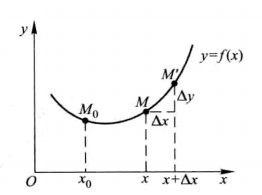
\includegraphics[width=.9\linewidth]{/media/wu/file/stuuudy/notes/images/miscellaneous/arc.png}
\end{center}
设函数\(f(x)\)在区间\((a,b)\)内具有连续导数,在曲线\(y=f(x)\)上取固定点
\(M_0(x_0,y_0)\)作为度量弧长的几点,并规定依\(x\)增大的方向作为曲线的争相,对
曲线上任一点\(M(x,y)\),规定有向弧度\(\arc{M_0M}\)的值\(s\)(简称为弧)如下:
\(s\)的绝对值的等于这弧段的长度,当有向弧段\(\arc{M_0M}\)的方向与曲线的正向一
致时,\(s>0\),相反时\(s<0\)

\begin{equation*}
\Delta s=\arc{M_0M'}-\arc{M_0M}=\arc{MM'}
\end{equation*}
于是
\begin{align*}
(\frac{\Delta s}{\Delta x})^2&=(\frac{\arc{MM'}}{\Delta x})^2=
(\frac{\arc{MM'}}{\abs{MM'}})^2\cdot\frac{\abs{MM'}^2}{(\Delta x)^2}\\
&=(\frac{\arc{MM'}}{\abs{MM'}})^2\cdot\frac{(\Delta x)^2+(\Delta y)^2}{(\Delta x)^2}\\
&=(\frac{\arc{MM'}}{\abs{MM'}})^2[1+(\frac{\Delta y}{\Delta x})^2]
\end{align*}
因此
\begin{equation*}
\frac{\Delta s}{\Delta x}=\pm\sqrt{(\frac{\arc{MM'}}{\abs{MM'}})^2\cdot[1+(\frac{\Delta y}{\Delta x})^2]}
\end{equation*}
令\(\Delta x\to0\)取极限,由于\(\Delta x\to0\)时,\(M'\to M\),这时弧的长度与弦的长度之
比的极限等于 1,即
\begin{equation*}
\lim_{M'\to M}\frac{\abs{\arc{MM'}}}{\abs{MM'}}=1
\end{equation*}
又
\begin{equation*}
\lim_{\Delta x\to0}\frac{\Delta y}{\Delta x}=y'
\end{equation*}
因此
\begin{equation*}
\frac{ds}{dx}=\pm\sqrt{1+y'^2}
\end{equation*}
由于\(s=s(x)\)是单调增加函数,于是有
\begin{equation*}
ds=\sqrt{1+y'^2}dx
\end{equation*}
\begin{equation*}
ds^2=dx^2+dy^2
\end{equation*}

\begin{center}
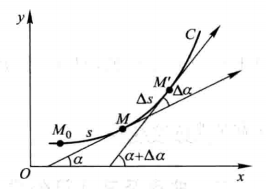
\includegraphics[width=.9\linewidth]{/media/wu/file/stuuudy/notes/images/miscellaneous/ArcDegree.png}
\end{center}

在曲线\(C\)上选定一点\(M_0\)作为度量弧\(s\)的基点,设曲线上点\(M\)对应与弧
\(s\),在点\(M\)处切线的倾角为\(\alpha\),曲线上另外一点\(M'\)对应于弧
\(s+\Delta s\),在点\(M'\)处切线的倾角为\(\alpha+\Delta \alpha\),则弧段
\(\arc{MM'}\)的长度为\(\abs{\Delta s}\)

我们用比值\(\abs{\frac{\Delta \alpha}{\Delta s}}\)来表达弧段\(\arc{MM'}\)的平均弯曲程度,叫
做弧段\(\arc{MM'}\)的 \textbf{平均曲率} ,并记作\(\bbar{K}\)

\begin{center}
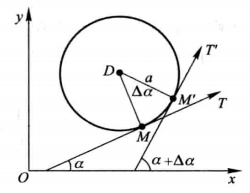
\includegraphics[width=.9\linewidth]{/media/wu/file/stuuudy/notes/images/miscellaneous/ArcCircle.png}
\end{center}

设圆的半径是\(a\),\(\angle MDM'=\frac{\Delta s}{a}\),因此
\begin{equation*}
\frac{\Delta\alpha}{\Delta s}=\frac{\frac{\Delta s}{a}}{\Delta s}=\frac{1}{a}
\end{equation*}
从而
\begin{equation*}
K=\abs{\frac{d\alpha}{d s}}=\frac{1}{a}
\end{equation*}

设曲线的直角坐标方程是\(y=f(x)\),且\(f(x)\)具有二阶导数,因为
\(\tan\alpha=y'\),所以
\begin{gather*}
\sec^2\alpha\frac{d\alpha}{dx}=y''\\
\frac{d\alpha}{dx}=\frac{y''}{1+\tan^2\alpha}=\frac{y''}{1+y'^2}
\end{gather*}
于是
\begin{equation*}
d\alpha=\frac{y''}{1+y'^2}dx
\end{equation*}
又因为
\begin{equation*}
ds=\sqrt{1+y'^2}dx
\end{equation*}
因此
\begin{equation*}
K=\frac{\abs{y''}}{(1+y'^2)^{3/2}}
\end{equation*}


\begin{center}
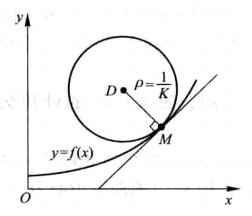
\includegraphics[width=.9\linewidth]{/media/wu/file/stuuudy/notes/images/miscellaneous/CurvatureCircle.png}
\end{center}
设曲线\(y=f(x)\)在点\(M(x,y)\)处的曲率为\(K(K\neq0)\),在点\(M\)处的曲线的法
线上,在凹的一侧取一点\(D\),使\(\abs{DM}=\frac{1}{K}=\rho\),以\(D\)为圆心,
\(\rho\) 为半径作圆,这个圆叫做曲线在点\(M\)处的 \textbf{曲率圆} ,\(D\)为 \textbf{曲率中心} , \(\rho\) 为曲
率半径
\section{不定积分}
\label{sec:org7560f94}
\subsection{不定积分的概念与性质}
\label{sec:org117f305}
\begin{definition}[]
如果 在区间\(I\)上,可导函数\(F(x)\)的导函数为\(f(x)\),那么函数\(F(x)\)就称
为\(f(x)\)在区间\(I\)上的一个 \textbf{原函数}
\end{definition}

\begin{theorem}[原函数存在定理]
如果函数\(f(x)\)在区间\(I\)上连续,那么在区间\(I\)上存在可导函数\(F(x)\),使
对任一\(x\in I\)都有
\begin{equation*}
F'(x)=f(x)
\end{equation*}
\end{theorem}

\begin{definition}[]
在区间\(I\)上,函数\(f(x)\)的带有任意常数项的原函数称为\(f(x)\)在区间\(I\)上
的 \textbf{不定积分} ,记为
\begin{equation*}
\int f(x)dx
\end{equation*}
其中\(\int\)称为 \textbf{积分号} , \(f(x)\)称为 \textbf{被积函数} ,\(f(x)dx\) 称为 \textbf{被积表达
式} ,\(x\)称为 \textbf{积分变量}
\end{definition}

\begin{equation*}
\int f(x)dx=F(x)+C
\end{equation*}

\textbf{基本积分表}
\begin{align*}
\int kdx&=kx+C(k\text{ is a constant})\\
\int x^\mu dx&=\frac{x^{\mu+1}}{\mu+1}+C(\mu\neq-1)\\
\int \frac{dx}{x}&=\ln\abs{x}+C\\
\int\frac{dx}{1+x^2}&=\arctan x+C\\
\int\frac{dx}{\sqrt{1-x^2}}&=\arcsin x+C\\
\int\cos xdx&=\sin x+C\\
\int \sin xdx&=-\cos x+C\\
\int\frac{dx}{\cos^2x}&=\int\sec^2xdx=\tan x+C\\
\int\frac{dx}{\sin^2x}&=\int\csc^2xdx=-\cot x+C\\
\int\sec x\tan xdx&=\sec x+C\\
\int\csc x\cot xdx&=-\csc x+C\\
\int e^xdx&=e^x+C\\
\int a^xdx&=\frac{a^x}{\ln a}+C\\
\end{align*}

\begin{proposition}[]
设函数\(f(x)\)及\(g(x)\)的原函数存在,则
\begin{equation*}
\int[f(x)+g(x)]dx=\int f(x)dx+\int g(x)dx
\end{equation*}
\end{proposition}

\begin{proposition}[]
设函数\(f(x)\)的原函数存在,\(k\)为非零常数,则
\begin{equation*}
\int kf(x)dx=k\int f(x)dx
\end{equation*}
\end{proposition}
\subsection{换元积分法}
\label{sec:org5602ebe}
\subsubsection{第一类换元法}
\label{sec:org3109d98}
\begin{theorem}[]
设\(f(u)\)具有原函数,\(u=\varphi(x)\)可导,则有换元公式
\begin{equation*}
\int f[\varphi(x)]\varphi'(x)dx=\left[\int f(u)du\right]_{u=\varphi(x)}
\end{equation*}
\end{theorem}

\begin{proposition}[]
\(\int\frac{1}{3+2x}dx\)
\end{proposition}

\begin{proof}
let \(u=3+2x\)

\begin{align*}
\int\frac{1}{3+2x}dx&=\int\frac{1}{2}\cdot\frac{1}{3+2x}(3+2x)'dx=\int\frac{1}{2}\cdot\frac{1}{u}du\\
&=\frac{1}{2}\ln\abs{u}+C
\end{align*}
\end{proof}

\begin{proposition}[]
\(\int\frac{1}{a^2+x^2}dx(a\neq0)\)
\end{proposition}

\begin{proof}
\begin{align*}
\int\frac{1}{a^2+x^2}dx&=\int\frac{1}{a^2}\cdot\frac{1}{1+(\frac{x}{a})^2}dx\\
&=\frac{1}{a}\int\frac{1}{1+(\frac{x}{a})^2}d\frac{x}{a}=\frac{1}{a}\arctan\frac{x}{a}+C
\end{align*}
\end{proof}

\begin{proposition}[]
\(\int\frac{1}{x^2-a^2}dx(a\neq0)\)
\end{proposition}

\begin{proof}
\begin{equation*}
\frac{1}{x^2-a^2}=\frac{1}{2a}(\frac{1}{x-a}-\frac{1}{x+a})
\end{equation*}
\end{proof}

\begin{proposition}[]
\(\int\sin^2x\cos^4xdx\)
\end{proposition}

\begin{proof}
\begin{align*}
\int\sin^2x\cos^4xdx&=\frac{1}{8}\int(1-\cos2x)(1+\cos2x)^2dx\\
&=\frac{1}{8}\int(1+\cos2x-\cos^22x-\cos^32x)dx\\
&=\frac{1}{8}\int(\cos2x-\cos^32x)dx+\frac{1}{8}\int(1-\cos^22x)dx\\
&=\frac{1}{8}\int\sin^22x\cdot\frac{1}{2}d(\sin2x)+\frac{1}{8}\int\frac{1}{2}(1-\cos4x)dx\\
&=\frac{1}{48}\sin^32x+\frac{x}{16}-\frac{1}{64}\sin4x+C
\end{align*}
\end{proof}

\begin{proposition}[]
\(\int\sec^6xdx\)
\end{proposition}

\begin{proof}
\begin{align*}
\int\sec^6xdx=\int(\sec^2x)^2\sec^2xdx=\int(1+\tan^2x)^2d(\tan x)
\end{align*}
\end{proof}

\begin{proposition}[]
\(\int\tan^5x\sec^3xdx\)
\end{proposition}

\begin{proof}
\begin{align*}
\int\tan^5x\sec^3xdx&=\int\tan^4x\sec^2x\sec x\tan xdx\\
&=\int(sec^2-1)^2\sec^2xd(\sec x)
\end{align*}
\end{proof}

\begin{proposition}[]
\(\int\csc xdx\)
\end{proposition}

\begin{proof}
\begin{align*}
\int\csc xdx&=\int\frac{dx}{\sin x}=\int\frac{dx}{2\sin\frac{x}{2}\cos\frac{x}{2}}\\
&=\int\frac{d(\frac{x}{2})}{\tan{\frac{x}{2}}{\cos^2\frac{x}{2}}}=
\int\frac{d(\tan\frac{x}{2})}{\tan\frac{x}{2}}=\ln\abs{\tan\frac{x}{2}}+C
\end{align*}
Since
\begin{equation*}
\tan\frac{x}{2}=\frac{1-\cos x}{\sin x}=\csc x-\cot x
\end{equation*}
we have
\begin{equation*}
\int\csc xdx=\ln\abs{\csc x-\cot x}+C
\end{equation*}
\end{proof}

\begin{proposition}[]
\(\int\sec xdx\)
\end{proposition}

\begin{proof}
\begin{align*}
\int\sec xdx&=\int\csc(x+\frac{\pi}{2})d(x+\frac{\pi}{2})\\
&=\ln\abs{\csc(x+\frac{\pi}{2})-\cot(x+\frac{\pi}{2})}+C\\
&=\ln\abs{\sec(x)+\tan(x)}+C
\end{align*}
\end{proof}
\subsubsection{第二类换元法}
\label{sec:orgab750ee}
\begin{theorem}[]
设\(x=\psi(t)\)是单调的可导函数,且\(\psi'(t)\neq0\),又设
\(f[\psi(t)]\psi'(t)\)具有原函数,则有
\begin{equation*}
\int f(x)dx=\left[\int f[\psi(t)]\psi'(t)dt\right]_{t=\psi^{-1}(x)}
\end{equation*}
其中\(\psi^{-1}(x)\)是\(x=\psi(t)\)的反函数
\end{theorem}

\begin{proposition}[]
\(\int\sqrt{a^2-x^2}dx(a>0)\)
\end{proposition}

\begin{proof}
let \(x=a\sin t,-\pi/2<t<\pi/2\), hence
\begin{equation*}
\int\sqrt{a^2-x^2}dx=\int a\cos t\cdot a\cos tdt=a^2\int\cos^2tdt=a^2(t/2+\sin2t/4)+C
\end{equation*}
and \(t=\arcsin\frac{x}{a}\)
\begin{equation*}
\int\sqrt{a^2-x^2}dx=\frac{a^2}{2}\arcsin\frac{x}{a}+\frac{1}{2}x\sqrt{a^2-x^2}+C
\end{equation*}
\end{proof}

\begin{proposition}[]
\(\int\frac{dx}{\sqrt{x^2+a^2}}\)
\end{proposition}

\begin{proof}
let \(x=a\tan t(-\pi/2<t<\pi/2)\), \(dx=a\sec^2tdt\)
hence
\begin{equation*}
\int\frac{dx}{\sqrt{x^2+a^2}}=\int\sec tdt=\ln\abs{\sec t+\tan t}+C
\end{equation*}
Hence
\begin{equation*}
\int\frac{dx}{\sqrt{x^2+a^2}}=\ln(\frac{x}{a}+\frac{\sqrt{x^2+a^2}{a}})+C=\ln(x+\sqrt{x^2+a^2})+C'
\end{equation*}
\end{proof}

\begin{proposition}[]
\(\int\frac{dx}{x^2-a^2}\)
\end{proposition}

\begin{proof}
since \(\sec^2t-1=\tan^2t\)

if \(x>a\), let \(x=a\sec t(0<t<\pi/2)\), \(dx=a\sec t\tan tdt\)

\begin{align*}
\int\frac{dx}{\sqrt{x^2-a^2}}&=\int\sec tdt=\ln(\sec t+\tan t)+C\\
&=\ln(x+\sqrt{x^2-a^2})+C'
\end{align*}

else if \(x<-a\)

consequently
\begin{equation*}
\int\frac{dx}{\sqrt{x^2-a^2}}=\ln\abs{x+\sqrt{x^2-a^2}}+C
\end{equation*}
\end{proof}

\begin{proposition}[]
\(\int\frac{dx}{\sqrt{1+x-x^2}}\)
\end{proposition}

\begin{proof}
    \begin{align*}
\int\frac{dx}{\sqrt{1+x-x^2}}&=\int\frac{d(x-1/2)}{\sqrt{(\sqrt{5}/2)^2-(x-1/2)^2}}\\
&=\arcsin\frac{2x-1}{\sqrt{5}}+C
\end{align*}
\end{proof}


\begin{proposition}[]
\(\int\frac{x^3}{(x^2-2x+2)^2}dx\)
\end{proposition}

\begin{proof}
let \(x-1=\tan t(-\pi/2<t<\pi/2)\)
\begin{equation*}
x^2-2x+2=\sec^2t, dx=\sec^2tdt
\end{equation*}
\end{proof}
\subsection{分布积分法}
\label{sec:org38c2169}
\begin{gather*}
uv'=(uv)'-u'v\\
\int uv'dx=uv-\int u'vdx\\
\int udv=uv-\int vdu
\end{gather*}

\begin{proposition}[]
\(\int x\cos xdx\)
\end{proposition}

\begin{proof}
\begin{equation*}
\int x\cos xdx=x\sin x-\int\sin xdx
\end{equation*}
\end{proof}

\begin{proposition}[]
\(\int\arccos xdx\)
\end{proposition}

\begin{proof}
\begin{align*}
\int\arccos xdx&=x\arccos x-\int xd(\arccos x)\\
&=x\arccos x+\int\frac{x}{\sqrt{1-x^2}}dx\\
&=x\arccos x-\frac{1}{2}\int\frac{1}{(1-x^2)^{0.5}}d(1-x^2)\\
&=x\arccos x-\sqrt{1-x^2}+C
\end{align*}
\end{proof}

\begin{proposition}[]
\(\int e^x\sin xdx\)
\end{proposition}

\begin{proof}
\begin{align*}
\int e^x\sin xdx&=e^x\sin x -\int\cos xd(e^x)\\
&=e^x\sin x-e^x\cos x-\int e^x\sin xdx
\end{align*}
Hence
\begin{equation*}
\int e^x\sin xdx=\frac{1}{2}e^x(\sin x-\cos x)+C
\end{equation*}
\end{proof}

\begin{proposition}[]
\(\int\sec^3xdx\)
\end{proposition}

\begin{proof}
\begin{align*}
\int\sec^3xdx&=\int\sec xd(\tan x)\\
&=\sec x\tan x-\int\sec x\tan t^2xdx\\
&=\sec x\tan x-\int\sec x(\sec^2x-1)dx\\
&=\sec x\tan x-\int\sec^3dx+\int\sec xdx\\
&=\sec x\tan x+\ln\abs{\sec x+\tan x}-\int\sec^3xdx
\end{align*}
\end{proof}
\subsection{有理函数的积分}
\label{sec:orgb71b099}
\begin{proposition}[]
\(\int\frac{1+\sin x}{\sin x(1+\cos x)}dx\)
\end{proposition}

\begin{proof}
\begin{gather*}
\sin x=2\sin \frac{x}{2}\cos\frac{x}{2}=\frac{2\tan\frac{x}{2}}{\sec^2\frac{x}{2}}=
\frac{2\tan\frac{x}{2}}{1+\tan^2\frac{x}{2}}\\
\cos x=\cos^2\frac{x}{2}-\sin^2\frac{x}{2}=\frac{1-\tan^2\frac{x}{2}}{\sec^2\frac{x}{2}}=
\frac{1-\tan^2\frac{x}{2}}{1+\tan^2\frac{x}{2}}
\end{gather*}
let \(u=\tan\frac{x}{2}\), \(dx=\frac{2}{1+u^2}u\)
\end{proof}
\section{定积分}
\label{sec:org4e11d44}
\subsection{定积分的概念与性质}
\label{sec:orgc465eed}
\begin{definition}[]
设函数\(f(x)\)在\([a,b]\)上有界,在\([a,b]\)中任意插入若干个分点
\begin{equation*}
a=x_0<x_1<\dots<x_n=b
\end{equation*}
把区间\([a,b]\)分成\(n\)个小区间
\begin{equation*}
[x_0,x_1],\dots,[x_{n-1},x_n]
\end{equation*}
各个小区间的长度依次为
\begin{equation*}
\Delta x_1=x_1-x_0,\dots,\Delta x_n=x_n-x_{n-1}
\end{equation*}
在每个小区间\([x_{i-1},x_i]\)上任取一点\(\xi_i(x_{i-1}\le\xi\le x_i)\),作函
数值\(f(\xi_i)\)与小区间长度\(\Delta x_i\)的乘积\(f(\xi_i)\Delta x_i(i=1,2,\dots,n)\),
并作出和
\begin{equation*}
S=\sum_{i=1}^nf(\xi_i)\Delta x_i
\end{equation*}
记\(\lambda=\max\{\Delta x_1,\dots,\Delta x_n\}\),如果当\(\lambda\to0\)时,这和的极限
总存在,且与闭区间\([a,b]\)的分法及点\(\xi_i\)的取法无关,那么称这个极限\(I\)
为函数\(f(x)\)在区间\([a,b]\)上的 \textbf{定积分} ,记作\(\int_a^bf(x)dx\),即
\begin{equation*}
\int_a^bf(x)dx=I=\lim_{\lambda\to0}\sum_{i=1}^nf(\xi_i)\Delta x_i
\end{equation*}
其中\(f(x)\)叫做 \textbf{被积函数} ,\(f(x)dx\)叫做 \textbf{被积表达式} ,\(x\)叫做 \textbf{积分分量} ,
\(a\)叫做 \textbf{积分下限} ,\(b\)记作 \textbf{积分上限} ,\([a,b]\)记作 \textbf{积分空间}
\end{definition}

\begin{theorem}[]
设\(f(x)\)在区间\([a,b]\)上连续,则\(f(x)\)在\([a,b]\)上可积
\end{theorem}

\begin{theorem}[]
设\(f(x)\)在区间\([a,b]\)上有界,且只有有限个间断点,则\(f(x)\)在\([a,b]\)上
可积
\end{theorem}

\begin{equation*}
\int_a^bf(x)dx=-\int_b^af(x)dx
\end{equation*}

\begin{proposition}[]
若 \(\alpha\) 与 \(\beta\) 均为常数,则
\begin{equation*}
\int_a^n[\alpha f(x)+\beta g(x)]dx=\alpha\int_a^bf(x)dx+\beta\int_a^b g(x)dx
\end{equation*}
\end{proposition}

\begin{proof}
\begin{align*}
\int_a^b[\alpha f(x)+\beta g(x)]dx&=\lim_{\lambda\to0}\sum_{i=1}^n[\alpha f(\xi_i)+\beta g(\xi_i)]\Delta x_i\\
&=\lim_{\lambda\to0}\alpha\sum_{i=1}^nf(\xi_i)\Delta x_i+
\lim_{\lambda\to0}\beta\sum_{i=1}^n g(\xi_i)\Delta x_i\\
&=\alpha\int_a^bf(x)dx+\beta\int_a^bg(x)dx
\end{align*}
\end{proof}

\begin{proposition}[]
设 \(a<c<b\),则
\begin{equation*}
\int_a^bf(x)dx=\int_a^cf(x)dx+\int_c^bf(x)dx
\end{equation*}
\end{proposition}

\begin{proposition}[]
如果在区间\([a,b]\)上\(f(x)\equiv1\),那么
\begin{equation*}
\int_a^b1dx=\int_a^bdx=b-a
\end{equation*}
\end{proposition}

\begin{proposition}[]
如果在区间\([a,b]\)上\(f(x)\ge0\),那么
\begin{equation*}
\int_a^bf(x)dx\ge0\quad(a<b)
\end{equation*}
\end{proposition}

\begin{corollary}[]
如果在区间\([a,b]\)上\(f(x)\le g(x)\),那么
\begin{equation*}
\int_a^bf(x)dx\le\int_a^bg(x)dx\quad(a<b)
\end{equation*}
\end{corollary}

\begin{corollary}[]
\(\abs{\int_a^bf(x)dx}\le\int_a^b\abs{f(x)}dx\)
\end{corollary}

\begin{proposition}[]
设\(M\)及\(m\)分别是函数\(f(x)\)在区间\([a,b]\)上的最大值及最小值,则
\begin{equation*}
m(b-a)\le\int_a^bf(x)dx\le M(b-a)\quad(a<b)
\end{equation*}
\end{proposition}

\begin{theorem}[定积分中值定理]
如果函数\(f(x)\)在积分区间\([a,b]\)上连续,那么在\([a,b]\)上至少存在一点 \(\xi\) ,
使得
\begin{equation*}
\int_a^bf(x)dx=f(\xi)(b-a)\quad(a\le\xi\le b)
\end{equation*}
\end{theorem}
\subsection{微积分基本公式}
\label{sec:org40aeb8a}
记
\begin{equation*}
\Phi(x)=\int^x_af(t)dt\quad(a\le x\le b)
\end{equation*}

\begin{theorem}[]
如果函数\(f(x)\)在区间\([a,b]\)上连续,那么积分上限的函数
\begin{equation*}
\Phi(x)=\int_a^xf(t)dt
\end{equation*}
在\([a,b]\)上可导,且
\begin{equation*}
\Phi'(x)=\frac{d}{dx}\int_a^xf(t)dt=f(x)\quad(a\le x\le b)
\end{equation*}
\end{theorem}

\begin{theorem}[]
如果函数\(f(x)\)在区间\([a,b]\)上连续,则函数
\begin{equation*}
\Phi(x)=\int_a^xf(t)dt
\end{equation*}
就是\(f(x)\)在\([a,b]\)上的一个原函数
\end{theorem}

\begin{theorem}[微积分基本定理]
如果函数\(F(x)\)是连续函数\(f(x)\)在区间\([a,b]\)上的一个原函数,那么
\begin{equation*}
\int_a^bf(x)dx=F(b)-F(a)
\end{equation*}
\end{theorem}
\subsection{定积分的换元法和分部积分法}
\label{sec:org6c49b3f}
\begin{theorem}[]
假定函数\(f(x)\)在区间\([a,b]\)上连续,函数\(x=\varphi(t)\)满足
\begin{enumerate}
\item \(\varphi(\alpha)=a,\varphi(\beta)=b\)
\item \(\varphi(t)\)在\([a,b]\)上具有连续导数,且其值域\(R_\varphi=[a,b]\),则有
\begin{equation*}
\int_a^bf(x)dx=\int_\alpha^\beta f[\varphi(t)]\varphi'(t)dt
\end{equation*}
\end{enumerate}
\end{theorem}

\begin{proposition}[]
Prove
\begin{enumerate}
\item 若\(f(x)\)在\([-a,a]\)上连续且为偶函数,则
\begin{equation*}
\int_{-a}^af(x)dx=2\int_0^af(x)dx
\end{equation*}
\item 若\(f(x)\)在\([-a,a]\)上连续且为奇函数,则
\begin{equation*}
\int_{-a}^af(x)dx=0
\end{equation*}
\end{enumerate}
\end{proposition}

\begin{proof}
令\(x=-t\)
\begin{equation*}
\int_{-a}^0f(x)dx=-\int_{a}^0f(-t)dt=\int_0^af(-t)dt=\int_0^af(-x)dx
\end{equation*}
\end{proof}

\begin{proposition}[]
设\(f(x)\)在\([0,1]\)上连续,证明
\begin{enumerate}
\item \(\int_0^{\frac{\pi}{2}}f(\sin x)dx=\int_0^{\frac{\pi}{2}}f(\cos x)dx\)
\item \(\int_0^\pi xf(\sin x)dx=\frac{\pi}{2}\int_0^\pi f(\sin x)dx\)
\end{enumerate}


计算
\begin{equation*}
\int_0^\pi\frac{x\sin x}{1+\cos^2x}dx
\end{equation*}
\end{proposition}

\begin{proof}
\begin{enumerate}
\item 设\(x=\frac{\pi}{2}-t\)
\begin{align*}
\int_0^{\frac{\pi}{2}}f(\sin x)dx&=-\int_{\frac{\pi}{2}}^0f[\sin(\frac{\pi}{2}-t)]dt\\
&=\int_0^{\frac{\pi}{2}}f(\cos t)dt
\end{align*}
\item 令\(x=\pi-t\)
\begin{align*}
\int_0^\pi xf(\sin x)dx&=-\int_\pi^0(\pi-t)f(\sin(\pi-t))dt\\
&=\int_0^\pi(\pi-t)f(\sin t)dt\\
&=\pi\int_0^\pi f(\sin x)dx-\int_0^\pi xf(\sin x)dx
\end{align*}
\end{enumerate}
\end{proof}

\begin{proposition}[]
\(\int_0^3\frac{x^2}{(x^2-3x+3)^2}dx\)
\end{proposition}

\begin{proof}
\(x^2-3x+3=(x-1.5)^3+3/4\). let \(x-1.5=\frac{\sqrt{3}}{2}\tan
   u(\abs{u}<\pi/2)\).
\begin{equation*}
(x^2-3x+3)^2=(\frac{3}{4}\sec^2u)^2,dx=\frac{\sqrt{3}}{2}\sec^2udu
\end{equation*}
\end{proof}

\begin{align*}
\int_a^bu(x)v'(x)dx&=\left[\in u(x)v'(x)dx
\right]^b_a\\
&=\left[u(x)v(x)-\int v(x)u'(x)dx\right]_a^b\\
&=[u(x)v(x)]^b_a-\int^b_av(x)u'(x)dx
\end{align*}
\subsection{反常积分}
\label{sec:org2a74cc4}
设函数\(f(x)\)在区间\([a,+\infty)\)上连续,取\(t>a\),作定积分
\(\int_a^tf(x)dx\),再求极限
\begin{equation*}
\lim_{t\to+\infty}\int^t_af(x)dx
\end{equation*}
称为 \textbf{函数\(f(x)\)在无穷区间\([a,+\infty)\)上的反常积分} ,记作
\(\int_a^{+\infty}f(x)dx\)

\begin{definition}[]
设函数\(f(x)\)在区间\([a,+\infty)\)上连续,如果极限存在,那么称反常积分收敛,
并称此极限为反常积分的值,若不存在,那么反常积分发散

设函数\(f(x)\)在区间\((-\infty,+\infty)\)上连续,如果反常积分
\(\int_{-\infty}^0f(x)dx\)与反常积分\(\int_0^{+\infty}f(x)dx\)均收敛,那么称
反常积分\(\int_{-\infty}^{+\infty}\)收敛,
\end{definition}

设\(F(x)\)为\(f(x)\)在\([a,+\infty)\)上的原函数,若\(\lim_{x\to+\infty}F(x)\)
存在,则反常积分
\begin{equation*}
\int_a^{+\infty}f(x)dx=\lim_{x\to+\infty}F(x)-F(a)
\end{equation*}
若不存在,则反常积分发散

\begin{proposition}[]
\(\int_{-\infty}^{+\infty}\frac{dx}{1+x^2}\)
\end{proposition}

\begin{proof}
\begin{equation*}
\int_{-\infty}^{+\infty}\frac{dx}{1+x^2}=[\arctan x]^{+\infty}_{-\infty}=\pi
\end{equation*}
\end{proof}

\begin{proposition}[]
\(\int_0^{+\infty}te^{-pt}dx,p>0\)
\end{proposition}

\begin{proof}
\begin{align*}
\int_0^{+\infty}te^{-pt}dt&=[-\frac{1}{p}\int td(e^{-pt})]^{+\infty}_0\\
&=[-\frac{t}{p}e^{-pt}+\frac{1}{p}\int e^{-pt}dt]^{+\infty}_0\\
&=\frac{1}{p^2}
\end{align*}
\end{proof}

如果函数\(f(x)\)在点\(a\)的任意邻域内都无界,那么点\(a\)称为函数\(f(x)\)的 \textbf{瑕
点}  (也称无界间断点), 无界函数的反常积分又称为 \textbf{瑕积分}

设函数\(f(x)\)在区间\((a,b]\)上连续,点\(a\)为\(f(x)\)的瑕点,任取\(t>a\),作
定积分\(\int_t^bf(x)dx\),再求极限
\begin{equation*}
\lim_{t\to a^+}\int^b_tf(x)dx
\end{equation*}

\begin{definition}[]
如果极限存在,那么称反常积分 \(\int_a^bf(x)dx\)收敛,并称此极限为该反常积分的
值
\end{definition}

设函数\(f(x)\)在区间\([a,c)\)及区间\((c,b]\)上连续,\(c\)为\(f(x)\)的瑕点,反
常积分\(\int_a^cf(x)dx+\int_c^bf(x)dx\)称为\(f(x)\)在区间\([a,b]\)上的反常积
分

\begin{proposition}[]
\(\int_0^a\frac{dx}{\sqrt{a^2-x^2}}dx(a>0)\)
\end{proposition}

\begin{proof}
\begin{equation*}
\int_0^a\frac{dx}{\sqrt{a^2-x^2}}=[\arcsin\frac{x}{a}]^a_0=\lim_{x\to a^-}
\arcsin \frac{x}{a}-0=\pi/2
\end{equation*}
\end{proof}
\section{定积分的应用}
\label{sec:org85e1523}
\subsection{定积分的元素法}
\label{sec:org3b94aa4}
\subsection{定积分在几何学上的应用}
\label{sec:org247f6ed}
\begin{examplle}[]
求椭圆\(\frac{x^2}{a^2}+\frac{y^2}{b^2}=1\)所围成的面积
\end{examplle}

\begin{proof}
利用椭圆的参数方程
\begin{equation*}
\begin{cases}
x=a\cos t \\
y=b\sin t
\end{cases},\quad (0\le t\le\frac{\pi}{2})
\end{equation*}
令\(x=a\cos t\),则
\begin{equation*}
y=b\sin t,dx=-a\sin t dt
\end{equation*}
当\(x\)由 0 变到\(a\)时,\(t\)由\(\pi/2\)变到 0,所以
\begin{align*}
A&=\int_{\pi/2}^0b\sin t(-a\sin t)dt=4ab\int_0^{\pi/2}\sin^2tdt=\pi ab
\end{align*}
\end{proof}

\begin{center}
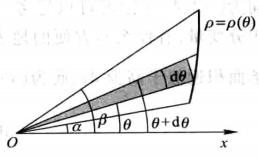
\includegraphics[width=5cm]{/media/wu/file/stuuudy/notes/images/miscellaneous/PolarCoordinate.png}
\end{center}

在极座标,设曲线\(\rho=\rho(\theta)\)及射线\(\theta=\alpha,\theta=\beta\)围成一个
曲边扇形,现在计算它的面积

取极角 \(\theta\) 为积分变量,它的变化空间为\([\alpha,\beta]\),相应与任意小区间
\([\theta,\theta+d\theta]\)的窄曲边扇形的面积可以用半径为\(\rho=\rho(\theta)\)、中心角
为\(d\theta\)的扇形的面积来近似,即
\begin{equation*}
dA=\frac{1}{2}[\rho(\theta)]^2d\theta
\end{equation*}
做定积分
\begin{equation*}
A=\int_\alpha^\beta\frac{1}{2}[\rho(\theta)]^2d\theta
\end{equation*}
\section{微分方程}
\label{sec:orgd06bc0c}
\subsection{微分方程的基本概念}
\label{sec:orgbfc564d}
\subsection{可分离变量的微分方程}
\label{sec:org7c5f483}
讨论一阶微分方程
\begin{equation*}
y'=f(x,y)
\end{equation*}

若一阶微分方程能写成
\begin{equation*}
g(y)dy=f(x)dx
\end{equation*}
的形式,原方程称为 \textbf{可分离变量的微分方程}
\subsection{齐次方程}
\label{sec:orgb1dadaf}
若一阶微分方程可化成
\begin{equation*}
\frac{dy}{dx}=\varphi(\frac{y}{x})
\end{equation*}
的形式,那么就称这方程为 \textbf{齐次方程}

引入新的未知函数
\begin{equation*}
u=\frac{y}{x}
\end{equation*}
就有
\begin{gather*}
y=ux,\frac{dy}{dx}=u+x\frac{du}{dx}\\
u+x\frac{du}{dx}=\varphi(u)\\
x\frac{du}{dx}=\varphi(u)-u\\
\frac{du}{\varphi(u)-u}=\frac{dx}{x}
\end{gather*}
\subsection{一阶线性微分方程}
\label{sec:orgebb1269}
\begin{equation*}
\frac{dy}{dx}+P(x)y=Q(x)
\end{equation*}
叫做 \textbf{一阶线性微分方程} ,若 \(Q(x)=\equiv0\),就称为  \textbf{齐次} 的,不然是 \textbf{非齐次}
的

对于非齐次线性方程,先考虑
\begin{equation*}
\frac{dy}{dx}+P(x)y=0
\end{equation*}
叫做对应于非齐次线性方程的 \textbf{齐次线性方程} ,我们有
\begin{gather*}
\frac{dy}{y}=-P(x)dx\\
\ln\abs{y}=-\int P(x)dx+C_1\\
y=Ce^{-\int P(x)dx}(C=\pm e^{C_1})
\end{gather*}

现在使用 \textbf{常数变易法} ,把通解中的\(C\)换成\(x\)的未知函数\(u(x)\),作变换
\begin{equation*}
y=ue^{-\int P(x)dx}
\end{equation*}
于是
\begin{gather*}
\frac{dy}{dx}=u'e^{-\int P(x)dx}-uP(x)e^{-\int P(x)dx}\\
u'e^{-\int P(x)dx}-uP(x)e^{-\int P(x)dx}+P(x)ue^{-\int P(x)dx}=Q(x)\\
u'e^{-\int P(x)dx}=Q(x),u'=Q(x)e^{\int P(x)dx}\\
u=\int Q(x)e^{\int P(x)dx}dx+C
\end{gather*}
因此
\begin{equation*}
y=e^{-\int P(x)dx}   (\int Q(x)e^{\int P(x)dx}dx+C)
\end{equation*}

\begin{proposition}[]
求方程
\begin{equation*}
\frac{dy}{dx}-\frac{2y}{x+1}=(x+1)^{5/2}
\end{equation*}
的通解
\end{proposition}

\begin{proof}
这是一个非齐次线性方程,先求对应的齐次方程的通解
\begin{gather*}
\frac{dy}{dx}-\frac{2y}{x+1}=0\\
\frac{dy}{y}=\frac{2dx}{x+1}\\
\ln\abs{y}=2\ln\abs{x+1}+C_1\\
y=C(x+1)^2(C=\pm e^{C_1})
\end{gather*}
令
\begin{equation*}
y=u(x+1)^2
\end{equation*}
那么
\begin{equation*}
\frac{dy}{dx}=u'(x+1)^2+2u(x+1)
\end{equation*}
代入非齐次方程得
\begin{equation*}
u'=\sqrt{x+1}
\end{equation*}
两端积分,得
\begin{equation*}
u=\frac{2}{3}(x+1)^{3/2}+C
\end{equation*}
因此
\begin{equation*}
y=(x+1)^2[\frac{2}{3}(x+1)^{3/2}+C]
\end{equation*}
\end{proof}



\begin{proposition}[]


\begin{center}
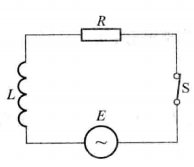
\includegraphics[width=.9\linewidth]{/media/wu/file/stuuudy/notes/images/miscellaneous/Circuit.png}
\end{center}
Consider a circuit. 其电源电动势为 \(E=E_m\sin\omega t\)(\(E_m,\omega\)都是
常量),电阻\(R\)和电感\(L\)都是常量,求电流\(i(t)\)
\end{proposition}

\begin{proof}
当电流变化时,\(L\)上有感应电动势\(-L\frac{di}{dt}\),由回路电压定律得出
\begin{equation*}
E-L\frac{di}{dt}-iR=0
\end{equation*}
即
\begin{equation*}
\frac{di}{dt}+\frac{R}{L}i=\frac{E}{L}
\end{equation*}
代入得
\begin{equation*}
 \frac{di}{dt}+\frac{R}{L}i=\frac{E_m}{L}\sin\omega t
\end{equation*}
同时\(i(t)\)满足初值
\begin{equation*}
i|_{t=0}=0
\end{equation*}
\end{proof}
\subsection{可降阶的高阶微分方程}
\label{sec:org357e6af}
\subsubsection{\(y^{(n)=f(x)}\)型微分方程}
\label{sec:org3c59cb5}
\begin{gather*}
y^{(n-1)}\int f(x)dx+C_1\\
y^{(n-2)}=\int[\int f(x)dx+C_1]dx+C_2\\
\vdots\\
\end{gather*}

\begin{proposition}[]
质量为\(m\)的质点受力\(F\)的作用沿\(Ox\)轴做直线运动,设力\(F=F(t)\)在开始时
刻\(t=0\)时\(F(0)=F_0\),随着时间\(t\)的增大,力\(F\)均匀地减小,直到\(t=T\)
时,\(F(T)=0\),如果开始时质点位于原点,且初速度为零,求这质点的运动规律
\end{proposition}

\begin{proof}
\begin{equation*}
F(t)=m\frac{d^2x}{dt^2}
\end{equation*}
\end{proof}
\subsubsection{\(y''=f(x,y')\)型的微分方程}
\label{sec:orgbe0ba85}
令\(y'=p\),则
\begin{equation*}
p'=f(x,p)
\end{equation*}
设其通解为
\begin{equation*}
p=\varphi(x,C_1)
\end{equation*}
但是\(p=\frac{dy}{dx}\),因此
\begin{equation*}
\frac{dy}{dx}=\varphi(x,C_1)
\end{equation*}
于是有通解
\begin{equation*}
y=\int\varphi(x,C_1)dx+C_2
\end{equation*}

\begin{proposition}[]
求微分方程
\(1+x^2y''=2xy'\) 满足初值
\begin{equation*}
y|_{x=0}=1,y'|_{x=0}=3
\end{equation*}
的特解
\end{proposition}

\begin{proof}
令\(y'=p\)
\begin{gather*}
\frac{dp}{p}=\frac{2x}{1+x^2}dx\\
\ln\abs{p}=\ln(1+x^2)+C\\
p=y'=C_1(1+x^2) (C_1=\pm e^C)\\
C_1=3(y'_{x=0}=3)\\
y'=3(1+x^2)\\
y=x^3+3x+C_2\\
C_2=1\\
y=x^3+3x+1
\end{gather*}
\end{proof}

\begin{proposition}[]
设有一均匀、柔软的绳索,两端固定,绳索仅受中立的作用下垂,试问该绳索在平衡状
态时是怎样的曲线
\end{proposition}

\begin{proof}
\begin{center}
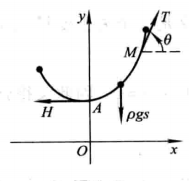
\includegraphics[width=.9\linewidth]{/media/wu/file/stuuudy/notes/images/miscellaneous/Rope.png}
\end{center}

设绳索的最低点为\(A\),取\(y\)轴通过\(A\)点铅直向上,并取\(x\)轴水平向右,
且\(\abs{OA}\)等于某个定值。设绳索曲线的方程为\(y=\varphi(x)\),考察绳索上点
\(A\)到另一点\(M(x,y)\)间的一段弧\(\arc{AM}\),设其长为\(s\),假定绳索的线密
度为 \(\rho\) ,则弧\(\arc{AM}\)所受重力为\(\rho gs\)。由于绳索时柔软的,因而在点\(A\)
处的张力沿水平的切线方向,其大小设为\(H\);在点\(M\)处的张力沿该点处的切线方
向,设其倾角为 \(\theta\) ,其大小为 \(T\) ,因作用于弧段 \(arc{AM}\) 的外力相互平衡,
得
\begin{equation*}
T\sin\theta=\rho gs, T\cos\theta=H
\end{equation*}
将两式相除,得
\begin{equation*}
\tan\theta=\frac{s}{a}(a=\frac{H}{\rho g})
\end{equation*}
由于\(\tan\theta=y',s=\int^x_0\sqrt{1+y'^2}dx\),代入得
\begin{equation*}
y'=\frac{1}{a}\int^x_0\sqrt{1+y'^2}dx
\end{equation*}
对 x 求导,得
\begin{equation*}
y''=\frac{1}{a}\sqrt{1+y'^2}
\end{equation*}
初值条件
\begin{equation*}
y|_{x=0}=a,y'|_{x=0}=0
\end{equation*}
设\(p=y'\),则
\begin{gather*}
p'=\frac{1}{a}\sqrt{1+p}\\
\frac{dp}{\sqrt{1+p^2}}=\frac{dx}{a}\\
\ln(p+\sqrt{1+p^2})=\frac{x}{a}+C_1\\
\end{gather*}
代入初值得\(C_1=0\)
解得
\begin{equation*}
p=\frac{1}{2}(e^{\frac{x}{a}}-e^{-\frac{x}{a}})
\end{equation*}
因此
\begin{equation*}
y=\frac{a}{2}(e^{\frac{x}{a}}+e^{-\frac{x}{a}})
\end{equation*}
\end{proof}
\subsubsection{\(y''=f(y,y')\)型的微分方程}
\label{sec:org183d347}
令\(y'=p\),则
\begin{equation*}
p\frac{dp}{dy}=f(y,p)
\end{equation*}
设它的通解为\(y'=p=\varphi(y,C_1)\)
则
\begin{equation*}
\int\frac{dy}{\varphi(y,C_1)}=x+C_2
\end{equation*}

\begin{proposition}[]
求微分方程
\begin{equation*}
yy''-y'^2=0
\end{equation*}
的通解
\end{proposition}

\begin{proof}
设 \(y'=p\)
\begin{equation*}
y''=\frac{dp}{dx}==\frac{dp}{dy}\cdot\frac{dy}{dx}=p\frac{dp}{dy}
\end{equation*}
因此
\begin{equation*}
yp\frac{dp}{dy}-p^2=0
\end{equation*}
在\(y\neq0,p\neq0\)时约去\(p\)并分离变量
\begin{gather*}
\frac{dp}{p}=\frac{dy}{y}\\
\ln\abs{p}=\ln\abs{y}+C\\
p=C_1y(C_1=\pm e^C)\\
\ln\abs{y}=C_1+C_2'\\
y=C_2e^{C_1x}(C_2=\pm e^{C_2'})
\end{gather*}
\end{proof}
\subsection{高阶线性微分方程}
\label{sec:orga95363e}
先讨论二阶齐次线性方程
\begin{equation*}
y''+P(x)y'+Q(x)y=0
\end{equation*}
\begin{theorem}[]
如果函数\(y_1(x)\)与函数\(y_2(x)\)二阶齐次线性方程的两个解,则
\begin{equation*}
y=C_1y_1(x)+C_2y_2(x)
\end{equation*}
也是一个解,\(C_1,C_2\)是任意常数
\end{theorem}

设\(y_1(x),\dots,y_n(x)\)为定义在区间\(I\)上的\(n\)个函数,如果存在\(n\)个不
全为零的常数\(k_1,k_2,\dots,k_n\)使得当\(x\in I\)时有恒等式
\begin{equation*}
k_1y_1+\dots+k_ny_n\equiv0
\end{equation*}
成立,那么就称这\(n\)个函数在区间\(I\)上 \textbf{线性相关} ;否则称 \textbf{线性无关}

\begin{theorem}[]
如果\(y_1(x)\)与\(y_2(x)\)是方程两个线性无关的特解,那么
\begin{equation*}
y=C_1y_1(x)+C_2y_2(x)
\end{equation*}
是方程的通解
\end{theorem}

\begin{corollary}[]
如果\(y_1(x),\dots,y_n(x)\)是\(n\)阶齐次线性方程
\begin{equation*}
y^{(n)}+a_1(x)y^{(n-1)}+\dots+a_{n-1}(x)y'+a_n(x)y=0
\end{equation*}
的\(n\)个线性无关的解,那么此方程的通解为
\begin{equation*}
y=C_1y_1(x)+C_2y_2(x)+\dots+C_ny_n(x)
\end{equation*}
其中\(C_1,\dots,C_n\)为任意常数
\end{corollary}

\begin{theorem}[]
设\(y^*(x)\)是二阶非齐次线性方程
\begin{equation*}
y''+P(x)y'+Q(x)y=f(x)
\end{equation*}
的一个特解,\(Y(x)\)是\(y''+P(x)y'+Q(x)y=0\)的通解,则
\begin{equation*}
y=Y(x)+y^*(x)
\end{equation*}


是二阶非齐次线性微分方程的通解
\end{theorem}

\begin{theorem}[叠加原理]
设非齐次线性方程的右端\(f(x)=f_1(x)+f_2(x)\),而\(y_1^*(x)\)与\(y_2^*(x)\)分
别是方程
\begin{equation*}
y''+P(x)y'+Q(x)y=f_1(x)
\end{equation*}
与
\begin{equation*}
y''+P(x)y'+Q(x)y=f_2(x)
\end{equation*}
的特解,则\(y_1^*(x)+y_2^*(x)\)就是原方程的特解
\end{theorem}
\subsection{常系数齐次线性微分方程}
\label{sec:orgc738a9e}
二阶齐次线性方程
\begin{equation*}
y''+P(x)y'+Q(x)y=0
\end{equation*}
中,如果\(y',y\)的系数\(P(x),Q(x)\)均为常数
\begin{equation}
y''+py'+qy=0\label{eq7-2}
\end{equation}
那么称为 \textbf{二阶常系数齐次线性微分方程} ,如果 \(p,q\)不全为常数,称为 \textbf{二阶变系数
齐次线性方程}

要找微分方程的通解,可以先求出它的两个解\(y_1,y_2\),如果它们线性无关,那么
\(y=C_1y_1+C_2y_2\)的通解

将\(y=e^{rx}\)求导,得
\begin{equation*}
y'=re^{rx},\quad y''=r^2e^{rx}
\end{equation*}
代入方程得
\begin{equation*}
(r^2+pr+q)e^{rx}=0
\end{equation*}
由于\(e^{rx}\neq0\),所以
\begin{equation}
r^2+pr+q=0\label{eq7-3}
\end{equation}
因此只要\(r\)满足代数方程\(r^2+pr+q=0\),函数\(y=e^{rx}\)就是微分方程的解,
称方程 \eqref{eq7-3}
为 方程 \eqref{eq7-2} \textbf{的 特征方程}

特征方程 \eqref{eq7-3} 的两个根
\begin{equation*}
r_{1,2}=\frac{-p\pm\sqrt{p^2-4q}}{2}
\end{equation*}
有三种不同情形
\begin{enumerate}
\item 当 \(p^2-4q>0\)时,\(r_1,r_2\)是两不相等的实根

\(y_1=e^{r_1x},y_2=e^{r_2x}\)是微分方程 \eqref{eq7-2} 的两个解,且
\(\frac{y_2}{y_1}=e^{(r_2-r_1)x}\) 不是常数,因此微分方程 \eqref{eq7-2} 的通
解为
\begin{equation*}
y=C_1e^{r_1x}+C_2e^{r_2x}
\end{equation*}
\item 当\(p^2-4q=0\)时,\(r_1,r_2\)是两个相等的实根

这时只得到 \eqref{eq7-2} 的一个解
\begin{equation*}
y_1=e^{r_1x}
\end{equation*}
这时还需另一个解\(y_2\),设\(\frac{y_2}{y_1}=u(x)\),即
\(y_2=e^{r_1x}u(x)\)
\begin{gather*}
y'_2=e^{r_1x}(u'+r_1u)\\
y''_2=e^{r_1x}(u''+2r_1u'+r_1^2u)
\end{gather*}
将\(y_2,y_2',y_2''\)代入微分方程 \eqref{eq7-2} 得
\begin{gather*}
e^{r_1x}[(u''+2r_1u'+r_1^2u)+p(u'+r_1u)+qu]=0\\
u''+(2r_1+p)u'+(r_1^2+pr_1+q)u=0
\end{gather*}
由于 \(r_1\)是特征方程 \eqref{eq7-3} 的二重根,因此\(r_1^2+pr_1+q=0\),且
\(2r_1+p=0\),于是
\begin{equation*}
u''=0
\end{equation*}
因为这里只要得到一个不为常数的解,不妨取\(u=x\),由此得到微分方程的另一个
解
\begin{equation*}
y_2=xe^{r_1x}
\end{equation*}
从而通解为
\begin{equation*}
y=(C_1+C_2x)e^{r_1x}
\end{equation*}
\item 当\(p^2-4q<0\)时,\(r_1,r_2\)是一对共轭复根
\begin{equation*}
r_1=\alpha+\beta i,\quad r_2=\alpha-\beta i
\end{equation*}
其中
\begin{equation*}
\alpha=-\frac{p}{2},\beta=\frac{\sqrt{4q-p^2}}{2}
\end{equation*}

利用欧拉公式\(e^{i\theta}=\cos\theta+i\sin\theta\)
\begin{gather*}
y_1=e^{(\alpha+\beta i)x}=e^{\alpha x}(\cos\beta x+i\sin\beta x)\\
y_2=e^{(\alpha-\beta i)x}=e^{\alpha x}(\cos\beta x-i\sin\beta x)
\end{gather*}

由于\(y_1,y_2\)有共轭关系,且方程 \eqref{eq7-2} 的解符合叠加原理,所以实值函
数
\begin{gather*}
\bbar{y_1}=\frac{1}{2}(y_1+y_2)=e^{\alpha x}\cos\beta x\\
\bbar{y_2}=\frac{1}{2i}(y_1-y_2)=e^{\alpha x}\sin\beta x
\end{gather*}
还是微分方程 \eqref{eq7-2} 的解,且\(\frac{\bbar{y_1}}{\bbar{y_2}}=\cot
      \beta x\),不是常数,所以微分方程的通解为
\begin{equation*}
y=e^{\alpha x}(C_1\cos\beta x+C_2\sin\beta x)
\end{equation*}
\end{enumerate}


综上所述,二阶常系数齐次线性微分方程 \eqref{eq7-2} 的通解的步骤如下
\begin{enumerate}
\item 写出特征方程
\begin{equation*}
r^2+pr+q=0
\end{equation*}
\item 求出特征方程的两个根\(r_1,r_2\)
\item 根据解的不同情形
\begin{center}
\begin{tabular}{ll}
\(r_1,r_2\) & 通解\\
\(r_1\neq r_2\) & \(y=C_1e^{r_1x}+C_2e^{r_2x}\)\\
\(r_1=r_2\) & \(y=(C_1+C_2x)e^{r_1x}\)\\
\(r_{1,2}=\alpha\pm\beta i\) & \(y=e^{\alpha x}(C_1\cos\beta x+C_2\sin\beta x)\)\\
\end{tabular}
\end{center}
\end{enumerate}


\textbf{\(n\)阶常系数齐次线性微分方程} 的一般形式是
\begin{equation}
y^{(n)}+p_1y^{(n-1)}+\dots+p_{n-1}y'+p_ny=0
\label{eq7-12}
\end{equation}
其中 \(p_1,\dots,p_n\)都是常数

有时我们用记号\(D\)(叫做 \textbf{微分算子} )表示对\(x\)求导的运算\(\frac{d}{dx}\),
把\(\frac{dy}{dx}\)记作\(Dy\),把\(\frac{d^ny}{dx^n}\)记作\(D^ny\),并把方程
\eqref{eq7-12} 记作
\begin{equation}
(D^n+p_1D^{n-1}+\dots+p_{n-1}D+p_n)y=0
\label{eq7-13}
\end{equation}
记
\begin{equation*}
L(D)=D^n+p_1D^{n-1}+\dots+p_{n-1}D+p_n
\end{equation*}
\(L(D)\)叫做 \textbf{微分算子\(D\)的\(n\)次多项式} ,于是方程 \eqref{eq7-13} 记作
\begin{equation*}
L(D)y=0
\end{equation*}

\begin{equation*}
r^n+p_1r^{n-1}+\dots+p_{n-1}r+p_n=0
\end{equation*}
为 \textbf{特征方程}

\begin{center}
\begin{tabular}{ll}
根 & 通解中的对应项\\
单实根\(r\) & \(Ce^{rx}\)\\
一对单复根\(r_{1,2}=\alpha\pm\beta i\) & \(e^{\alpha x}(C_1\cos\beta x+C_2\sin\beta x)\)\\
\(k\)重实根 & \(e^{rx}(C_1+C_2x+\dots+C_kx^{k-1})\)\\
一对\(k\)重复根\(r_{1,2}=\alpha\pm\beta i\) & \(e^{\alpha x}[(C_1+C_2x+\dots+C_kx^{k-1})\cos\beta x+(D_1+D_2x+\dots+D_kx^{k-1})\sin\beta x]\)\\
\end{tabular}
\end{center}


\begin{proposition}[]
求方程\(y^{(4)}-2y'''+5y''=0\)的通解
\end{proposition}

\begin{proof}
特征方程
\begin{gather*}
r^4-2r^3+5r^2=0\\
r^2(r^2-2r+5)=0\\
r_1=r_2=0,r_{3,4}=1\pm 2i
\end{gather*}
因此通解
\begin{equation*}
y=C_1+C_2x+e^x(C_3\cos2x+C_4\sin2x)
\end{equation*}
\end{proof}
\subsection{常系数非齐次线性微分方程}
\label{sec:org155ad2d}
二阶常系数非齐次线性微分方程的一般形式
\begin{equation*}
y''+py'+qy=f(x)
\end{equation*}
其中\(p,q\)是常数

这里只需讨论求二阶常系数非齐次线性微分方程的一个特解\(y^*\)的方法

\textbf{待定系数法} ,\(f(x)\)的两种形式
\begin{enumerate}
\item \(f(x)=e^{\lambda x}P_m(x)\),其中\(\lambda\)是常数,\(P_m(x)\)是\(x\)的一个
\(m\)次多项式:
\begin{equation*}
P_m(x)=a_0x^m+a_1x^{m-1}+\dots+a_{m-1}x+a_m
\end{equation*}
\item \(f(x)=e^{\lambda x}[P_l(x)\cos\omega x+Q_n(x)\sin\omega x]\),其中 \(\lambda\) 、 \(\omega\) 是常
数,\(\omega\neq0\), \(P_l(x),Q_n(x)\)分别是\(x\)的\(l\)次、\(n\)次多项式,
且只有一个可为零
\end{enumerate}

\section{向量代数与空间解析几何}
\label{sec:org3424e7d}
\subsection{向量及其线性运算}
\label{sec:org07606d8}
\begin{theorem}[]
设向量\(\ba\neq\bzero\),则向量\(\bb\)平行于\(\ba\)的充分必要条件是:存在唯一
的实数 \(\lambda\) ,使 \(\bb=\lambda\ba\)
\end{theorem}



\begin{center}
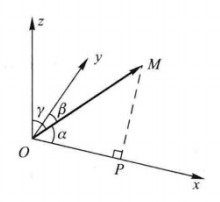
\includegraphics[width=4cm]{/media/wu/file/stuuudy/notes/images/miscellaneous/VectorAngle.png}
\end{center}

非零向量\(\br\)与三条坐标轴的夹角 \(\alpha\) 、 \(\beta\) 、 \(\gamma\) 称为\(\br\)的方向角,设
\(\vec{OM}=\br=(x,y,z)\)
\begin{gather*}
\cos\alpha=\frac{x}{\abs{OM}}=\frac{x}{\abs{\br}}\\
\cos\beta=\frac{y}{\abs{\br}},\cos\gamma=\frac{z}{\abs{\br}}\\
(\cos\alpha,\cos\beta,\cos\gamma)=\frac{\br}{\abs{\br}}=\be_r
\end{gather*}

\(\cos\alpha,\cos\beta,\cos\gamma\) 称为向量 \(\br\) 的 \textbf{方向余弦}

\begin{center}
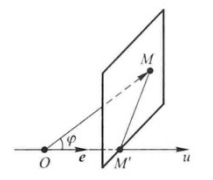
\includegraphics[width=4cm]{/media/wu/file/stuuudy/notes/images/miscellaneous/Projection.png}
\end{center}

设点\(O\)及单位向量\(\be\)确定\(u\) 轴,任给向量\(\br\),作\(\vec{OM}=\br\),
再过点\(M\)作与\(u\)轴垂直的平面交\(u\)轴于点\(M'\) (点\(M'\)叫做 \textbf{点\(M\)在 u
轴上的投影} ),则向量 \(\vec{OM'}\) 称为向量\(\br\)在\(u\)轴上的分向量,设
\(\vec{OM'}=\lambda\be\),则 \(\lambda\) 称为 \textbf{向量\(\br\)在\(u\)轴上的投影} ,记作 \((\br)_u\)
\subsection{数量积 向量积 混合积}
\label{sec:org8bfce5f}
\textbf{数量积} ,记作\(\ba\cdot\bb\)
\begin{equation*}
\ba\cdot\bb=\abs{\ba}\abs{\bb}\cos\theta
\end{equation*}

\begin{center}
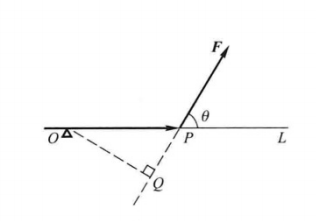
\includegraphics[width=4cm]{/media/wu/file/stuuudy/notes/images/miscellaneous/D1.png}
\end{center}
力\(\bF\)对支点\(O\)的力矩是一向量\(\bM\),它的模
\begin{equation*}
\abs{\bM}=\abs{OQ}\abs{\bF}=\abs{\vec{OP}}\abs{\bF}\sin\theta
\end{equation*}

设向量 \(\bc\)有两个向量\(\ba\)与\(\bb\)按下列方式定出:

\(\bc\)的模\(\abs{\bc}=\abs{\ba}\abs{\bb}\sin\theta\),其中 \(\theta\) 为\(\ba,\bb\)间
的夹角,\(\bc\)的方向垂直于\(\ba,\bb\)所决定的平面,称为 \textbf{向量积} ,记做
\(\ba\times\bb\)

按此定义,力矩\(\bM\)等于\(\vec{OP}\)与\(\bF\)的向量积

\begin{enumerate}
\item \(\ba\times\ba=-\ba\times\bb\)
\item \((\ba+\bb)\times\bc=\ba\times\bc+\bb\times\bc\)
\item \((\lambda\ba)\times\bb=\ba\times(\lambda\bb)=\lambda(\ba\times\bb)\)
\end{enumerate}


设\(\ba=a_x\bi+a_y\bj+a_z\bk,\bb=b_x\bi+b_y\bj+b_z\bk\),那么
\begin{align*}
\ba\times\bb&=
a_x\bi\times(b_x\bi+b_y\bj+b_z\bk)+\\
&a_y\bi\times(b_x\bi+b_y\bj+b_z\bk)+a_z\bi\times(b_x\bi+b_y\bj+b_z\bk)\\
&=a_xb_x(\bi\times\bi)+a_xb_y(\bi\times\bj)+a_xb_z(\bi\times\bk)+\\
&a_yb_x(\bj\times\bi)+a_yb_y(\bj\times\bj)+a_yb_z(\bj\times\bk)+\\
&a_zb_x(\bk\times\bi)+a_zb_y(\bk\times\bj)+a_zb_z(\bk\times\bk)+\\
&=(a_yb_z-a_zb_y)\bi+
(a_zb_x-a_xb_z)\bj+
(a_xb_y-a_yb_x)\bk
\end{align*}

可写成
\begin{equation*}
\ba\times\bb=
\begin{vmatrix}
\bi&\bj&\bk\\
a_x&a_y&a_z\\
b_x&b_y&b_z
\end{vmatrix}
\end{equation*}

设已知三个向量\(\ba,\bb,\bc\),\((\ba\times\bb)\cdot\bc\)称为三个向量的混合积,
记作\([\ba\bb\bc]\)

因为
\begin{equation*}
\ba\times\bb=
\begin{vmatrix}
\bi&\bj&\bk\\a_x&a_y&a_z\\\
b_x&b_y&b_z
\end{vmatrix}=
\begin{vmatrix}
a_y&a_z\\
b_y&b_z
\end{vmatrix}\bi-
\begin{vmatrix}
a_x&a_z\\
b_x&b_z
\end{vmatrix}\bj+
\begin{vmatrix}
a_x&a_y\\
b_x&b_y
\end{vmatrix}\bk
\end{equation*}
则
\begin{align*}
[\ba\bb\bc]&=(\ba\times\bb)\cdot\bc\\
&=
\begin{vmatrix}
a_y&a_z\\
b_y&b_z
\end{vmatrix}c_x-
\begin{vmatrix}
a_x&a_z\\
b_x&b_z
\end{vmatrix}c_y+
\begin{vmatrix}
a_x&a_y\\
b_x&b_y
\end{vmatrix}c_z=\\
&=
\begin{vmatrix}
a_x&a_y&a_z\\
b_x&b_y&b_z\\
c_x&c_y&c_z
\end{vmatrix}
\end{align*}
\subsection{平面及其方程}
\label{sec:orgfc76089}
如果曲面\(S\)与三元方程
\begin{equation*}
F(x,y,z)=0
\end{equation*}
有下述关系
\begin{enumerate}
\item 曲面\(S\)上任一点的坐标都满足方程
\item 不再曲面\(S\)上的点都不满足方程
\end{enumerate}


那么方程就叫做 \textbf{曲面\(S\)的方程}

如果一非零向量垂直于一平面,这向量就叫做该 \textbf{平面的法线向量}

因为过空间一点可以作而且只能作一平面垂直于一已知直线,所以当平面 \(\Pi\) 上一点
\(M_0(x_0,y_0,z_0)\)和它的一个法线向量 \(\bn=(A,B, C)\)为已知时,平面 \(\Pi\) 就确
定了

设\(M(x,y,z)\)是平面 \(\Pi\) 上任一点,则向量\(\vec{M_0M}\)必与\(\bn\)垂直,即它们
的数量积为 0
\begin{equation*}
\bn\cdot\vec{M_0M}=0
\end{equation*}
因此
\begin{equation*}
A(x-x_0)+B(y-y_0)+C(z-z_0)=0
\end{equation*}
这就是平面 \(\Pi\) 所满足的方程,叫做 \textbf{平面的点法式方程}

设有一三元一次方程
\begin{equation}
Ax+By+Cz+D=0\label{eq8.3.4}
\end{equation}
任取满足该方程的一组数\(x_0,y_0,z_0\),相减得
\begin{equation}
A(x-x_0)+B(y-y_0)+C(z-z_0)=0\label{eq8.3.6}
\end{equation}
方程 \eqref{eq8.3.4} 称为 \textbf{平面的一般方程} ,其中\(x,y,z\)的系数就是该平面的一个
法线向量\(\bn\) 的坐标,即\(\bn=(A,B,C)\)

\begin{examplle}[]
设一平面与\(x,y,z\)轴的交点依次为\(P(a,0,0),Q(0,b,0),R(0,0,c)\)三点,如图

\begin{center}
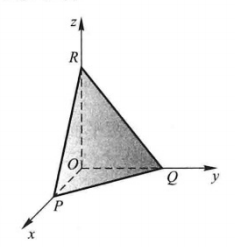
\includegraphics[width=4cm]{/media/wu/file/stuuudy/notes/images/miscellaneous/PlainCut.png}
\end{center}
设所求平面的方程为
\begin{equation*}
Ax+By+Cz+D=0
\end{equation*}
则
\begin{equation*}
\begin{cases}
aA+D=0\\bB+D=0\\cC+D=0
\end{cases}
\end{equation*}
解得
\begin{equation*}
\frac{x}{a}+\frac{y}{b}+\frac{z}{c}=1
\end{equation*}
叫做 \textbf{平面的截距式方程} ,\(a,b,c\)依次叫做平面在\(x,y,z\)轴上的 \textbf{截距}
\end{examplle}


两平面的法线向量的夹角(通常指锐角或直角)称为 \textbf{两平面的夹角}

设\(\Pi_1,\Pi_2\)的法线向量依次为\(\bn_1=(A_1,B_1,C_1),\bn_2=(A_2,B_2,C_2)\),
则平面\(\Pi_1,\Pi_2\)的夹角 \(\theta\) 应是 \(\la\bn_1,\b_2\ra\)和
\(\pi-\la\bn_1,\bn_2\ra\)中的锐角或直角

两平面的夹角 \(\theta\) 可由
\begin{equation*}
\cos\theta=
\frac{\abs{A_1A_2+B_1B_2+C_1C_2}}{\sqrt{A_1^2+B_1^2+C_1^2}\sqrt{A_2^2+B_2^2+C_2^2}}
\end{equation*}
来确定,因为\(\bn_1\cdot\bn_2=\abs{\bn_1}\abs{\bn_2}\cos\theta\)
\subsection{空间直线及其方程}
\label{sec:org07ecbb4}
空间直线\(L\)可以看作两个平面\(\Pi_1,\Pi_2\)的交线,因此
\begin{equation*}
\begin{cases}
A_1x+B_1y+C_2z+D_1=0\\
A_2x+B_2y+C_2z+D_2=0
\end{cases}
\end{equation*}
称为 \textbf{空间直线的一般方程}

如果一个非零向量平行于一条已知直线,那么这个向量就叫做这条直线的 \textbf{方向向量}

由于过空间一点可作而且只能作一条直线平行于一已知直线,所以当直线\(L\)上一点
\(M_0(x_0,y_0,z_0)\)和它的一方向向量\(\bs=(m,n,p)\)为已知时,直线\(L\)的位置
就完全确定了

设\(M(x,y,z)\)是直线\(L\)上任一点,则向量\(\vect{M_0M}\)于\(L\)的方向向量
\(\bs\)平行,因此
\begin{equation*}
\frac{x-x_0}{m}=\frac{y-y_0}{n}=\frac{z-z_0}{p}
\end{equation*}
这叫做 \textbf{直线的对称式方程} 或 \textbf{点向式方程} 。直线的任一方向向量\(\bs\)的坐标
\(m,n,p\)叫做这直线的一组 \textbf{方向数} ,而向量\(\bs\)的方向余弦叫做该直线的 \textbf{方向余
弦}

如设
\begin{equation*}
\frac{x-x_0}{m}=\frac{y-y_0}{n}=\frac{z-z_0}{p}=t
\end{equation*}
则
\begin{equation*}
\begin{cases}
x=x_0+mt\\y=y_0+nt\\z=z_0+pt
\end{cases}
\end{equation*}
就是 \textbf{直线的参数方程}

\begin{examplle}[]
用对称式方程及参数方程表示直线
\begin{equation*}
\begin{cases}
x+y+z+1=0\\  2x-y+3z+4=0
\end{cases}
\end{equation*}
先找出直线上的一点\(x_0,y_0,z_0\),如\(1,0,-2\)

下面再找出这直线的方向向量\(\bs\),取
\begin{equation*}
\bs=\bn_1\times\bn_2=
\begin{vmatrix}
\bi&\bj&\bk\\1&1&1\\2&-1&3
\end{vmatrix}=4\bi-\bj-3\bk
\end{equation*}
因此对称式方程
\begin{equation*}
\frac{x-1}{4}=\frac{y}{-1}=\frac{z+2}{-3}
\end{equation*}
\end{examplle}

两直线的方向向量的夹角(通常指锐角或直角)叫做 \textbf{两直线的夹角}

设\(L_1,L_2\)的方向向量依次为\(bs_1=(m_1,n_1,p_1),\bs_2=(m_2,n_2,p_2)\),则夹
角 \(\varphi\) 可由
\begin{equation*}
\cos\varphi=\frac{\abs{m_1m_2+n_1n_2+p_1p_2}}{\sqrt{m_1^2+n_1^2+p_1^2}\sqrt{m_2^2+
n_2^2+p_2^2}}
\end{equation*}
确定

当直线与平面不垂直时,直线和它再平面上的投影直线的夹角
\(\varphi(-\le\varphi\le\pi/2)\)称为 \textbf{直线与平面的夹角}

设直线的方向向量为\(\bs=(m,n,p)\),平面的法线向量为\(\bn=(A,B,C)\),直线与平
面的夹角为 \(\varphi\) ,则\(\sin\varphi=\abs{\cos\la\bs,\bn\ra}\)
\begin{equation*}
\sin\varphi=\frac{\abs{Am+Bn+Cp}}{
\sqrt{A^2+B^2+C^2}\sqrt{m^2+n^2+p^2}}
\end{equation*}
\subsection{曲面及其方程}
\label{sec:org958e52e}
以一条平面曲线绕其平面上的一条直线旋转一周所成的曲面叫做 \textbf{旋转曲面} ,旋转曲线
和定直线依次叫做旋转平面的 \textbf{母线} 和 \textbf{轴}

设在\(yOz\)坐标面上有一条已知直线\(C\),它的方程为
\begin{equation*}
f(y,z)=0
\end{equation*}
把这曲线绕\(z\)轴一周,就得到一个以\(z\)轴为轴的旋转曲面

设\(M_1(0,y_1,z_1)\)为曲线\(C\)上任一点,则有
\begin{equation*}
f(y_1,z_1)
\end{equation*}
当曲线\(C\)绕\(z\)轴旋转时,点\(M_1\)绕\(z\)轴转到另一点\(M(x,y,z)\),这时
\(z=z_1\),且点\(M\)到\(z\)轴的距离为
\begin{equation*}
d=\sqrt{x^2+y^2}=\abs{y_1}
\end{equation*}
将\(z_1=z,y_1=\pm\sqrt{x^2+y^2}\)代入得
\begin{equation*}
f(\pm\sqrt{x^2+y^2},z)=0
\end{equation*}
就是所求旋转曲面的方程

\begin{examplle}[]
直线\(L\)绕另一条与\(L\)相交的直线旋转一周,所得旋转曲面叫做 \textbf{圆锥面} ,两直线
的交点叫做 圆锥面的 \textbf{半顶角} ,若旋转轴为\(z\)轴,则在\(yOz\)坐标面上直线的方程
\begin{equation*}
z=y\cot\alpha
\end{equation*}
因此圆锥面
\begin{equation*}
z=\pm\sqrt{x^2+y^2}\cot\alpha
\end{equation*}
\end{examplle}

\(x^2+y^2=R^2\)叫做 \textbf{圆柱面} ,\(xOy\)面上的圆\(x^2+y^2=R^2\)叫做它的 \textbf{准线} ,平
行于\(z\)轴的直线\(l\)叫做它的 \textbf{母线}

一般的,直线\(L\)沿定曲线 \(C\)平行移动形成的轨迹叫做 \textbf{柱面} ,定曲线\(C\)叫做
\textbf{柱面的准线} ,动直线\(L\)叫做 \textbf{柱面的母线}

我们把三元二次方程\(F(x,y,z)=0\)所表示的曲面称为 \textbf{二次曲面} ,把平面称为 \textbf{一次曲
面}

二次曲面有九种
\begin{enumerate}
\item \textbf{椭圆锥面}  \(\frac{x^2}{a^2}+\frac{y^2}{b^2}=z^2\)

平面\(z=t\)与曲面\(F(x,y,z)=0\)的交线称为 \textbf{截痕}

在\(xOy\)平面上,把点\(M(x,y)\)变为点\(M'(x,\lambda y)\),从而把点\(M\)的轨迹
\(C\)变为点\(C'\),称为把图形\(C\)沿\(y\)轴方向伸缩 \(\lambda\) 倍变成图形\(C'\)。假
如\(C\)为曲线\(F(x,y)=0\),点\(M(x_1,y_1)\in C\),点\(M\)变为
\(M'(x_2,y_2)\),其中\(x_2=x_1,y_2=\lambda y_1\),故
\(F(x_2,\frac{1}{\lambda}y_2)\),因此点\(M'(x_2,y_2)\)的轨迹\(C'\)的方程为
\(F(x,\frac{1}{\lambda}y)=0\)。例如把圆\(x^2+y^2=a^2\)沿\(y\)轴方向伸缩
\(\frac{b}{a}\)倍,就变为椭圆\(\frac{x^2}{a^2}+\frac{y^2}{b^2}=1\)

\item 椭球面 \(\frac{x^2}{a^2}+\frac{y^2}{b^2}+\frac{z^2}{c^2}=1\)

\item 单叶双曲面 \(\frac{x^2}{a^2}+\frac{y^2}{b^2}-\frac{z^2}{c^2}=1\)

把\(xOz\)面上的双曲线\(\frac{x^2}{a^2}-\frac{z^2}{c^2}=1\)绕\(z\)轴旋转,
的旋转单叶双曲面\(\frac{x^2+y^2}{a^2}-\frac{z^2}{c^2}=1\),在把次旋转面沿
\(y\)轴方向神座\(\frac{b}{a}\)倍

\item 双叶双曲面 \(\frac{x^2}{a^2}-\frac{y^2}{b^2}-\frac{z^2}{c^2}=1\)

\item 椭圆抛物面 \(\frac{x^2}{a^2}+\frac{y^2}{b^2}=z\)

\item 双曲抛物面 \(\frac{x^2}{a^2}-\frac{y^2}{b^2}=z\)

又称 \textbf{马鞍面} 。用截痕法

用平面\(x=t\)截此曲面,所得截痕\(l\)为平面\(x=t\)上的抛物线
\begin{equation*}
-\frac{y^2}{b^2}=z-\frac{t^2}{a^2}
\end{equation*}
\end{enumerate}
\subsection{空间曲线及其方程}
\label{sec:org8f8f0af}
设
\begin{equation*}
F(x,y,z)=0,\quad G(x,y,z)=0
\end{equation*}
时两个曲面的方程,则
\begin{equation*}
\begin{cases}
F(x,y,z)=0\\
G(x,y,z)=0
\end{cases}
\end{equation*}
叫做 \textbf{空间曲线\(C\)的一般方程}
\section{多元函数微分法及其应用}
\label{sec:org57b6840}
\subsection{多元函数的基本概念}
\label{sec:org4f578cf}
设\(P_0(x_0,y_0)\)是\(xOy\)平面上的一个点, \(\delta\) 是某一正数,与点
\(P_0(x_0,y_0)\)距离小于 \(\delta\) 的点\(P(x,y)\)的全体,称为点\(P_0\)的 \(\delta\) \textbf{邻域} ,记
作\(U(P_0,\delta)\),即
\begin{equation*}
U(P_0,\delta)=\{P\mid\abs{PP_0}<\delta\}
\end{equation*}
也就是
\begin{equation*}
U(P_0,\delta)=\{(x,y)\mid\sqrt{(x-x_0)^2+(y-y_0)^2}<\delta\}
\end{equation*}

点\(P_0\)的去心 \(\delta\) 邻域,记作\(\interior{U}(P_0,\delta)\),即
\begin{equation*}
\interior{U}(P_0,\delta)=\{P\mid 0<\abs{PP_0}<\delta\}
\end{equation*}

任意一点\(P\in\R^2\)与任意一个点集\(E\subset\R^2\)有以下三种关系之一
\begin{enumerate}
\item \textbf{内点} :如果存在点\(P\)的某个邻域\(U(P)\),使\(U(P)\subset E\)
\item \textbf{外点} :如果存在点\(P\)的某个邻域\(U(P)\),使\(U(P)\cap E=\emptyset\)
\item \textbf{边界点} :如果点\(P\)的任一邻域内既有属于\(E\)的点,又有不属于\(E\)的点
\end{enumerate}


\(E\)的边界点的全体,称为\(E\)的 \textbf{边界} ,记作\(\partial E\)


\textbf{聚点} :如果对于任意给定的\(\delta>0\),点\(P\)的去心邻域\(\interior{U}(P,\delta)\)内总有
 \(E\)中的点,那么称\(P\)是\(E\)的聚点

\begin{itemize}
\item \textbf{开集} :如果点集\(E\)的点都是\(E\)的内点
\item \textbf{闭集} :如果点\(E\)的边界\(\partial E\subset E\),那么称\(E\)为闭集
\item \textbf{连通集} :如果点集\(E\)内任何两点,都可以用折线联接,且该折线上的点都属于
\(E\),那么称\(E\)为连通集
\item \textbf{区域} :连通的开集
\item \textbf{闭区域} :开区域连同它的边界
\end{itemize}


\begin{definition}[]
设\(D\)是\(\R^2\)的一个非空子集,称映射\(f:D\to\R\)为定义在\(D\)上的 \textbf{二元函
数} ,通常记为
\begin{equation*}
z=f(x,y),(x,y)\inD
\end{equation*}
或
\begin{equation*}
z=f(P),P\in D
\end{equation*}
其中点集\(D\)称为该函数的 \textbf{定义域} ,\(x\)和\(y\)称为 \textbf{自变量} ,\(z\)称为 \textbf{因变
量}
\end{definition}

\begin{definition}[]
设二元函数\(f(P)=f(x,y)\)的定义域为\(D\),\(P_0(x_0,y_0)\)是\(D\)的聚点,如果
存在常数\(A\)对于任意给定的正数 \(\epsilon\) ,总存在正数 \(\delta\) ,使得当点
\(P(x,y)\in D\cap\interior{U}(P_0,\delta)\)时,都有
\begin{equation*}
\abs{f(P)-A}=\abs{f(x,y)-A}<\epsilon
\end{equation*}
成立,那么就称常数\(A\)为函数\(f(x,y)\)当\((x,y)\to(x_0,y_0)\)时的极限,记作
\begin{equation*}
\lim_{(x,y)\to(x_0,y_0)}f(x,y)=A 
\end{equation*}
也记作
\begin{equation*}
\lim_{P\to P_0}f(P)=A
\end{equation*}
\end{definition}

考查函数
\begin{equation*}
f(x,y)=
\begin{cases}
\frac{xy}{x^2+y^2}&x^2+y^2\neq0\
0&x^2+y^2=0
\end{cases}
\end{equation*}
当点\(P(x,y)\)沿\(x\)轴趋于点\((0,0)\)时
\begin{equation*}
\lim_{\substack{(x,y)\to(x_0,y_0)\\y=0}}f(x,y)=\lim_{x\to0}f(x,0)=0\\
\end{equation*}
当 点\(P(x,y)\)沿\(y\)轴趋于点\((0,0)\)时
\begin{equation*}
\lim_{\substack{(x,y)\to(x_0,y_0)\\x=0}}f(x,y)=\lim_{y\to0}f(0,y)=0\\
\end{equation*}
虽然点\(P(x,y)\)以上述两种方式趋于原点时函数的极限存在且相等,但是
\(\lim_{(x,y)\to(0,0)}f(x,y)\)并不存在,因为当点\(P(x,y)\)沿着直线\(y=kx\)趋
于点\((0,0)\)时,有
\begin{equation*}
\lim_{\substacks{(x,y)\to(0,0)\\y=kx}}f(x,y)=
\lim_{x\to0}\frac{kx^2}{x^2+k^2x^2}=\frac{k}{1+k^2}
\end{equation*}

\begin{definition}[]
设二元函数\(f(P)=f(x,y)\)的定义域为\(D\),\(P_0(x_0,y_0)\)为\(D\)的聚点,且
\(P_0\in D\),如果
\begin{equation*}
\lim_{(x,y)\to(x_0,y_0)}f(x,y)=f(x_0,y_0)
\end{equation*}
那么称\(f(x,y)\)在点\(P_0(x_0,y_0)\)连续
\end{definition}

\begin{definition}[]
设函数\(f(x,y)\)的定义域为\(D\),\(P_0(x_0,y_0)\)是\(D\)的聚点,如果函数
\(f(x,y)\)在点\(P_0(x_0,y_0)\)不连续,那么称\(P_0\)为函数\(f(x,y)\)的间断点
\end{definition}

根据多元函数的极限运算法则,可以证明多元连续函数的和、差、积仍未连续函数;连
续函数的商在分母不为零处仍连续;多元连续函数的复合函数也是连续函数

一切多元初等函数在其定义区域内是连续的

由多元函数的连续性,如果要求它在点\(P_0\)处的极限,而该店又在此函数的定义区域
内,那么此极限值就是函数在该点的函数值
\begin{equation*}
\lim_{P\to P_0}f(P)=f(P_0)
\end{equation*}

\begin{proposition}[有界性与最大值最小值定理]
在有界闭区域\(D\)上的多元连续函数,必定在\(D\)上有界,且能取得它的最大值和最
小值
\end{proposition}

\begin{proposition}[介值定理]
在有界闭区域\(D\)上的多元连续函数必取得介于最大值和最小值之间的任何值
\end{proposition}
\subsection{偏导数}
\label{sec:org0bd9440}
\begin{definition}[]
设函数\(z=f(x,y)\)在点\((x_0,y_0)\)的某一邻域内有定义,当\(y\)固定在\(y_0\)而
\(x\)在\(x_0\)处有增量\(\Delta x\)时,相应的函数有增量
\begin{equation*}
f(x_0+\Delta x,y_0)-f(x_0,y_0)
\end{equation*}
如果
\begin{equation*}
\lim_{\Delta x\to0}\frac{f(x_0+\Delta x,y_0)-f(x_0,y_0)}{\Delta x}
\end{equation*}
存在,那么称此极限为函数\(z=f(x,y)\)在点\((x_0,y_0)\)处 \textbf{对\(x\)的偏导数} ,记
作
\begin{equation*}
\left.\frac{\partial z}{\partial x}\right\rvert_{\substacks{x=x_0\\y=y_0}},\quad
\left.\frac{\partial f}{\partial x}\right\rvert_{\substacks{x=x_0\\y=y_0}},\quad
z_x\Big\rvert_{\substacks{x=x_0\\y=y_0}},\text{ or }
f_x(x_0,y_0)
\end{equation*}
\end{definition}

如果函数\(z=f(x,y)\)在区域\(D\)内每一点\((x,y)\)处对\(x\)的偏导数都存在,那么
这个偏导数就是\(x,y\)的函数,它就称为函数\(z=f(x,y)\) \textbf{对自变量\(x\)的偏到函数}
,记作
\begin{equation*}
\frac{\partial z}{\partial x},\frac{\partial f}{\partial x},z,f_x(x,y)
\end{equation*}

设函数\(z=f(x,y)\)在区域\(D\)内具有偏导数
\begin{equation*}
\frac{\partial z}{\partial x}=f_x(x,y),\frac{\partial z}{\partial y}=f_y(x,y)
\end{equation*}
那么在\(D\)内\(f_x(x,y),f_y(x,y)\)都是\(x,y\)的函数,如果这两个函数的偏导数存
在,那么称它们是函数\(z=f(x,y)\)的 \textbf{二阶偏导数}

\begin{theorem}[]
如果函数\(z=f(x,y)\)的两个二阶混合偏导数\(\frac{\partial^2z}{\partial y\partial x}\)及
\(\frac{\partial^2z}{\partial x\partial y}\)在区域\(D\)内连续,那么在该区域内这两个二阶混合
偏导数必相等
\end{theorem}
\subsection{全微分}
\label{sec:orgc88f909}
\begin{definition}[]
设函数\(z=f(x,y)\)在点\((x,y)\)的某邻域内有定义,如果函数在点\((x,y)\)的全增
量
\begin{equation*}
\Delta z=f(x+\Delta x,y+y+\Delta)-f(x,y)
\end{equation*}
可表示为
\begin{equation*}
\Delta z=A\Delta x+B\Delta y+o(\rho)
\end{equation*}
其中\(A\)和\(B\)不依赖于\(\Delta x,\Delta y\)而仅与\(x,y\)有关,\(\rho=\sqrt{(\Delta x)^2+(\Delta
   y)^2}\),那么称\(z=f(x,y)\)在点\((x,y)\) \textbf{可微分} ,而\(A\Delta x+B\Delta y\)称
为函数\(z=f(x,y)\)在点\((x,y)\)的 \textbf{全微分} ,记作\(dz\),即
\begin{equation*}
dz=A\Delta x+B\Delta y
\end{equation*}
如果函数在区域内各点处都可微分,那么称函数 \textbf{在\(D\)内可微分}
\end{definition}

\begin{theorem}[必要条件]
如果函数\(z=f(x,y)\)在点\((x,y)\)可微分,那么该函数在点\((x,y)\)的偏导数
\(\frac{\partial z}{\partial x},\frac{\partial z}{\partial y}\)必定存在,且函数\(z=f(x,y)\)在点\((x,y)\)
的全微分为
\begin{equation*}
dz=\frac{\partial z}{\partial x}\Delta x+\frac{\partial z}{\partial y}\Delta y
\end{equation*}
\end{theorem}

\begin{proof}
令\(\Delta x,\Delta y\)分别等于 0
\end{proof}

\begin{theorem}[充分条件]
如果函数\(z=f(x,y)\)的偏导数\(\frac{\partial z}{\partial x},\frac{\partial z}{\partial y}\)在点\((x,y)\)
连续,那么该函数在该点可微分
\end{theorem}

\begin{proof}
由假定,函数的偏导数在点\(P(x,y)\)的某邻域内存在,设点\((x+\Delta x,y+\Delta
   y)\)为这邻域内任一一点,考察函数的全增量
\begin{align*}
\Delta z&=f(x+\Delta x,y+\Delta y)-f(x,y)\\
&=[f(x+\Delta x,y+\Delta y)-f(x,y+\Delta y)]+[f(x,y+\Delta y)-f(x,y)]
\end{align*}
应用拉格朗日中值定理
\begin{equation*}
f(x+\Delta x,y+\Delta y)-f(x,y+\Delta y)=f_x(x+\theta_1\Delta x,y+\Delta y)\Delta x(0<\theta_1<1)
\end{equation*}
又依假设\(f_x(x,y)\)在点\((x,y)\)连续,所以上式可写为
\begin{equation*}
f(x+\Delta x,y+\Delta y)-f(x,y+\Delta y)=f_x(x,y)\Delta x+\epsilon_1\Delta x
\end{equation*}
其中\(\epsilon_1\)为\(\Delta x\)与\(\Delta y\)的函数,且当\(\Delta x\to0,\Delta y\to0\)时,
\(\epsilon_1\to0\)
同理
\begin{equation*}
f(x,y+\Delta y)-f(x,y)=f_y(x,y)\Delta y+\epsilon_2\Delta y
\end{equation*}
因此
\begin{equation*}
\Delta z=f_x(x,y)\Delta x+f_y(x,y)\Delta y+\epsilon_1\Delta x+\epsilon_2\Delta y
\end{equation*}
容易看出
\begin{equation*}
\abs{\frac{\epsilon_1\Delta x+\epsilon_2\Delta y}{\rho}}\le\abs{\epsilon_1}+\abs{\epsilon_2}
\end{equation*}
随着\((\Delta x,\Delta y)\to(0,0)\)而趋于零
\end{proof}

通常把二元函数的全微分等于它的两个偏微分之和这件事称为二元函数的微分符合 \textbf{叠加
原理}

如果三元函数\(u=f(x,y,z)\)可微分,那么它的全微分
\begin{equation*}
du=\frac{\partial u}{\partial x}dx+\frac{\partial u}{\partial y}dy+\frac{\partial u}{\partial z}dz
\end{equation*}
\subsection{多元复合函数的求导法则}
\label{sec:org987a3e7}
\begin{theorem}[]
如果函数\(u=\varphi(t)\)及\(v=\psi(t)\)都在点\(t\)可导,函数\(z=f(u,v)\)在对
应点\((u,v)\)具有连续偏导数,那么复合函数\(z=f[\varphi(t),\psi(t)]\)在点\(t\)可导,且
\begin{equation*}
\frac{dz}{dt}=\frac{\partial z}{\partial u}\frac{du}{dz}+\frac{\partial z}{\partial v}\frac{dv}{dt}
\end{equation*}
\end{theorem}

\begin{proof}
\begin{gather*}
\Delta z=\frac{\partial z}{\partial u}\Delta u+\frac{\partial z}{\partial v}\Delta v+\epsilon_1\Delta u+\epsilon_2\Delta v\\
\frac{\Delta z}{\Delta t}=\frac{\partial z}{\partial u}\frac{\Delta u}{\Delta t}
+\frac{\partial z}{\partial v}\frac{\Delta v}{\Delta t}+\epsilon_1\frac{\Delta u}{\Delta t}+\epsilon_2\frac{\Delta v}{\Delta t}\\
\lim_{\Delta t\to0}\frac{\Delta z}{\Delta t}=\frac{\partial z}{\partial u}\frac{du}{dt}+\frac{\partial z}{\partial v}\frac{dv}{dt}
\end{gather*}
\end{proof}

\begin{theorem}[]
如果函数\(u=\varphi(x,y),v=\psi(x,y)\)都在点\((x,y)\)具有对\(x\)及对\(y\)的偏
导数,函数\(z=f(u,v)\)在对应点\((u,v)\)具有连续偏导数,那么复合函数
\(z=f(\varphi(x,y),\psi(x,y))\)在点\((x,y)\)的两个偏导数都存在,且
\begin{align*}
&\frac{\partial z}{\partial x}=\frac{\partial z}{\partial u}\frac{\partial u}{\partial x}+\frac{\partial z}{\partial v}\frac{\partial v}{\partial x}\\
&\frac{\partial z}{\partial y}=\frac{\partial z}{\partial u}\frac{\partial u}{\partial y}+\frac{\partial z}{\partial v}\frac{\partial v}{\partial y}
\end{align*}
\end{theorem}

\begin{theorem}[]
如果函数\(u=\varphi(x,y)\)在点\((x,y)\)具有对\(x\)及对\(y\)的偏导数,函数
\(v=\psi(y)\)在点\(y\)可导,函数\(z=f(u,v)\)在对应点\((u,v)\)具有连续偏导数,
那么复合函数\(z=f(\varphi(x,y),\psi(y))\)在点\((x,y)\)的两个偏导数都存在,且
\begin{align*}
&\frac{\partial z}{\partial x}=\frac{\partial z}{\partial u}\frac{\partial u}{\partial x}\\
&\frac{\partial z}{\partial y}=\frac{\partial z}{\partial u}\frac{\partial u}{\partial y}+\frac{\partial z}{\partial v}\frac{\partial v}{\partial y}
\end{align*}
\end{theorem}

\begin{proposition}[]
设\(u=f(x,y)\)的所有二阶偏导数连续,把下列表达式转换为极坐标系中的形式
\begin{enumerate}
\item \((\frac{\partial u}{\partial x})^2+(\frac{\partial u}{\partial y})^2\)
\item \(\frac{\partial^2u}{\partial x^2}+\frac{\partial^2u}{\partial y^2}\)
\end{enumerate}
\end{proposition}

\begin{proof}
由直角坐标与极坐标间的关系
\begin{equation*}
x=\rho\cos\theta,\quad y=\rho\sin\theta
\end{equation*}
于是
\begin{equation*}
u=f(x,y)=f(\rho\cos\theta,\rho\sin\theta)=F(\rho,\theta)
\end{equation*}
\begin{equation*}
\rho=\sqrt{x^2+y^2},\quad\theta=\artan\frac{y}{x}
\end{equation*}
求导
\begin{align*}
&\frac{\partial u}{\partial x}=\frac{\partial u}{\partial \rho}\frac{\partial \rho}{\partial x}+\frac{\partial u}{\partial \theta}\frac{\partial \theta}{\partial x}=
\frac{\partial u}{\partial\rho}\frac{x}{\rho}-\frac{\partial u}{\partial \theta}\frac{y}{\rho^2}=
\frac{\partial u}{\partial \rho}\cos\theta-\frac{\partial u}{\partial \theta}\frac{\sin\theta}{\rho}
\end{align*}
\end{proof}

设函数\(z=f(u,v)\)具有连续偏导数,则有全微分
\begin{equation*}
dz=\frac{\partial z}{\partial u}du+\frac{\partial z}{\partial v}dv
\end{equation*}
如果\(u,v\)又是中间变量,即\(u=\varphi(x,y),v=\psi(x,y)\),且这两个函数也具有
连续偏导数,那么复合函数的全微分为
\begin{equation*}
dz=\frac{\partial z}{\partial x}dx+\frac{\partial z}{\partial y}dy=\frac{\partial z}{\partial u}du+\frac{\partial z}{\partial v}dv
\end{equation*}
无论\(u,v\)时自变量还是中间变量,函数的全微分形式是一样的,这个性质叫 \textbf{全微分
形式不变性}
\subsection{隐函数的求导公式}
\label{sec:orgb6d0c97}
\begin{theorem}[隐函数存在定理 1]
设函数\(F(x,y)\)在点\(P(x_0,y_0)\)的某一邻域内具有连续偏导数,且
\(F(x_0,y_0)=0,F_y(x_0,y_0)\neq0\),则方程\(F(x,y)=0\)在点\((x_0,y_0)\)的某一
邻域内恒能唯一确定一个连续且具有连续导数的函数\(y=f(x)\),它满足条件
\(y_0=f(x_0)\),并有
\begin{equation*}
\frac{dy}{dx}=-\frac{F_x}{F_y}
\end{equation*}
\end{theorem}

因为由恒等式
\begin{equation*}
F(x,f(x))\equiv 0
\end{equation*}
求这个函数的全导数
\begin{equation*}
\frac{\partial F}{\partial x}+\frac{\partial F}{\partial y}\frac{dy}{dx}=0
\end{equation*}
因为\(F_y\)连续,且\(F_y(x_0,y_0)\neq0\),所以存在\((x_0,y_0)\)的一个邻域,在
这个邻域内\(F_y\neq0\),于是
\begin{equation*}
\frac{dy}{dx}=-\frac{F_x}{F_y}
\end{equation*}


\begin{proposition}[]
验证\(x^2+y^2-1=0\)在点\((0,1)\)的某一邻域内能唯一确定一个有连续导数,当
\(x=0,y=1\)时的隐函数\(y=f(x)\),并求这函数的一阶与二阶导数在\(x=0\)的值
\end{proposition}

\begin{proposition}[]
设\(F(x,y)=x^2+y^2-1\),则\(F_x=2x,F_y=2y,F(0,1)=0,F_y(0,1)=2\neq0\),因此由
定理可知,方程\(x^2+y^2-1=0\)在点\((0,1)\)的某邻域内能唯一确定一个有连续导数,
当\(x=0\),\(y=1\)时的函数\(y=f(x)\)

\begin{align*}
&\frac{dy}{dx}=-\frac{F_x}{F_y}=-\frac{x}{y}\\
&\frac{d^2y}{dx^2}=-\frac{y-xy'}{y^2}=-\frac{1}{y^3}
\end{align*}
\end{proposition}

\begin{theorem}[隐函数存在定理 2]
设函数\(F(x,y,z)\)在点\(P(x_0,y_0,z_0)\)的某一邻域内具有连续偏导数,且
\(F(x_0,y_0,z_0)=0, F_z(x_0,y_0,z_0)\neq0\),则方程\(F(x,y,z)=0\)在点
\((x_0,y_0,z_0)\)的某一邻域内恒能唯一确定一个连续且具有连续偏导数的函数
\(z=f(x,y)\),它满足条件\(z_0=f(x_0,y_0)\),并有
\begin{equation*}
\frac{\partial z}{\partial x}=-\frac{F_x}{F_z},\quad
\frac{\partial z}{\partial y}=-\frac{F_y}{F_z}
\end{equation*}
\end{theorem}

由于\(F(x,y,f(x,y))\equiv0\),将上式两端分别对\(x,y\)求导
\begin{equation*}
F_x+F_z\frac{\partial z}{\partial x}=0,F_y+F_z\frac{\partial z}{\partial y}=0
\end{equation*}

考虑方程组
\begin{equation*}
\begin{cases}
F(x,y,u,v)=0\\
G(x,y,u,v)=0
\end{cases}
\end{equation*}

\begin{theorem}[隐函数存在定理 3]
设\(F(x,y,u,v),G(x,y,u,v)\)在点\(P(x_0,y_0,u_0,v_0)\)的某一邻域内具有对各个变
量的连续偏导数,又\(F(x_0,y_0,u_0,v_0)=0,G(x_0,y_0,u_0,v_0)=0\),且偏导数所组
成的函数行列式(雅可比(Jacobi)式)
\begin{equation*}
J=\frac{\partial(F,G)}{\partial(u,v)}=
\begin{vmatrix}
\frac{\partial F}{\partial u}&\frac{\partial F}{\partial v}\\
\frac{\partial G}{\partial u}&\frac{\partial G}{\partial v}
\end{vmatrix}
\end{equation*}
在点\(P(x_0,y_0,u_0,v_0)\)不等于 0,则方程组\(F(x,y,u,v)=0,G(x,y,u,v)=0\)在点
\((x_0,y_0,u_0,v_0)\)的某一邻域内恒能唯一确定一组连续且具有连续偏导数的函数
\(u=u(x,y),v=v(x,y)\),它们满足条件\(u_0=u(x_0,y_0),v_0=v(x_0,y_0)\),并有
\begin{align*}
&\frac{\partial u}{\partial x}=-\frac{1}{J}\frac{\partial (F,G)}{\partial(x,v)}=-\frac{
\begin{vmatrix}
F_x&F_v\\
G_x&G_v
\end{vmatrix}}
{\begin{vmatrix}
F_u&F_v\\
G_u&G_v
 \end{vmatrix}}\\
&\frac{\partial v}{\partial x}=-\frac{1}{J}\frac{\partial (F,G)}{\partial(u,x)}=-\frac{
\begin{vmatrix}
F_u&F_x\\
G_u&G_x
\end{vmatrix}}
{\begin{vmatrix}
F_u&F_v\\
G_u&G_v
 \end{vmatrix}}\\
&\frac{\partial u}{\partial y}=-\frac{1}{J}\frac{\partial (F,G)}{\partial(y,v)}=-\frac{
\begin{vmatrix}
F_y&F_v\\
G_y&G_v
\end{vmatrix}}
{\begin{vmatrix}
F_u&F_v\\
G_u&G_v
 \end{vmatrix}}\\
&\frac{\partial v}{\partial y}=-\frac{1}{J}\frac{\partial (F,G)}{\partial(u,y)}=-\frac{
\begin{vmatrix}
F_u&F_y\\
G_u&G_y
\end{vmatrix}}
{\begin{vmatrix}
F_u&F_v\\
G_u&G_v
 \end{vmatrix}}\\
\end{align*}
\end{theorem}

由于
\begin{equation*}
F[x,y,u(x,y),v(x,y)]\equiv0,G[x,y,u(x,y),v(x,y)]\equiv0
\end{equation*}
则
\begin{equation*}
\begin{cases}
F_x+F_u\frac{\partial u}{\partial x}+F_v\frac{\partial v}{\partial x}=0\\
G_x+G_u\frac{\partial u}{\partial x}+G_v\frac{\partial v}{\partial x}=0
\end{cases}
\end{equation*}
因为行列式
\begin{equation*}
J=
\begin{vmatrix}
F_u&F_v\\G_u&G_v
\end{vmatrix}\neq0
\end{equation*}
从而解得
\begin{equation*}
\frac{\partial u}{\partial x}=-\frac{1}{J}\frac{\partial(F,G)}{\partial(x,v)},
\frac{\partial v}{\partial x}=-\frac{1}{J}\frac{\partial(F,G)}{\partial(u,x)}
\end{equation*}

\begin{proposition}[]
设\(xu-yv=0,yu+xv=1\),求\(\frac{\partial u}{\partial x},\frac{\partial u}{\partial y},\frac{\partial v}{\partial
   x},\frac{\partial v}{\partial y}\)
\end{proposition}

\begin{proof}
   
\end{proof}
\subsection{多元函数微分学的几何应用}
\label{sec:org227e55f}
空间曲线 \(\Gamma\) 的参数方程为
\begin{equation*}
\begin{cases}
x=\varphi(t)\\
y=\psi(t)\\
z=\omega(t)
\end{cases},t\in[\alpha,\beta]
\end{equation*}
若记
\begin{equation*}
\br=x\bi+y\bj+z\bk,\quad
\bff(t)=\varphi(t)\bi+\psi(t)\bj+\omega(t)\bk
\end{equation*}
则
\begin{equation*}
\br=\bff(t),t\in[\alpha,\beta]
\end{equation*}

\begin{definition}[]
设数集\(D\subset\R\),则称映射\(\bff:D\to\R^n\)为 \textbf{一元向量值函数} ,通常记为
\begin{equation*}
\br=\bff(t),t\in D
\end{equation*}
\end{definition}

\begin{definition}[]
设向量值函数\(\bff(t)\)在点\(t_0\)的某一去心邻域内有定义,如果存在一个常向量
\(\br_0\)对于任意给定的正数 \(\epsilon\) ,总存在正数 \(\delta\) 使得当\(t\)满足
\(0<\abs{t-t_0}<\delta\)时,对应的函数值\(\bff(t)\)都满足不等式
\begin{equation*}
\abs{\bff(t)-\br_0}<\epsilon
\end{equation*}
那么常向量\(\br_0\)就叫做 \textbf{向量值函数\(\bff(t)\)当\(t\to t_0\)时的极限} ,记作
\begin{equation*}
\lim_{t\to t_0}\bf(t)=\br_0
\end{equation*}
\end{definition}
   向量值函数\(\bff(t)\)当\(t\to t_0\)时的极限存在的充分必要条件是三个分量函数当
\(t\to t_0\)时的极限都存在,其极限为
\begin{equation*}
\lim_{t\to t_0}\bff(t)=\left(
\lim_{t\to t_0}f_1(t),\lim_{t\to t_0}f_2(t),\lim_{t\to t_0}f_3(t)
\right)
\end{equation*}

若
\begin{equation*}
\lim_{t\to t_0}\bff(t)=\bff(t_0)
\end{equation*}
则称向量值函数\(\bff(t)\)在\(t_0\)连续

\begin{definition}[]
设向量值函数\(\br=\bff(t)\)在点\(t_0\)的某一邻域内有定义,如果
\begin{equation*}
\lim_{\Delta t\to0}\frac{\Delta \br}{\Delta t}=\lim_{\Delta t\to0}
\frac{\bff(t_0+\Delta t)-\bff(t_0)}{\Delta t}
\end{equation*}
存在,那么就称这个极限向量为 \textbf{向量值函数\(\br=\bff(t)\)在\(t_0\)处的导数} 或
\textbf{导向量} ,记作 \(\bff'(t_0)\)或\(\left.\frac{d\br}{dt}\right\rvert_{t=t_0}\)
\end{definition}

向量值函数\(\bff(t)\)在\(t_0\)可导的充分必要条件是其三个分量函数在\(t_0\)可导
\begin{equation*}
\bff'(t_0)=f_1'(t_0)\bi+f_2'(t_0)\bj+f_3'(t_0)\bk
\end{equation*}

设\(\bu(t),\bv(t)\)是可导的向量值函数,\(\bC\)是常向量,\(c\)是任一常数,
\(\varphi(t)\)是可导的数量函数,则
\begin{enumerate}
\item \(\frac{d}{dt}\bC=\bzero\)
\item \(\frac{d}{dt}[c\bu(t)]=c\bu'(t)\)
\item \(\frac{d}{dt}[\bu[t]\pm\bv[t]]=\bu'(t)\pm\bv'(t)\)
\item \(\frac{d}{dt}[\varphi(t)\bu(t)]=\varphi'(t)\bu(t)+\varphi(t)\bu'(t)\)
\item \(\frac{d}{dt}[\bu(t)\cdot\bv(t)]=\bu'(t)\cdot\bv(t)+\bu(t)\cdot\bv'(t)\)
\item \(\frac{d}{dt}[\bu(t)\times\bv(t)]=\bu'(t)\times\bv(t)+\bu(t)\times\bv'(t)\)
\item \(\frac{d}{dt}\bu[\varphi(t)]=\varphi'(t)\bu'[\varphi(t)]\)
\end{enumerate}

t

设空间曲线 \(\Gamma\) 是向量值函数\(\br=\bf(t),t\in D\)的终端曲线,
\(\vect{OM}=\bff(t_0),\vect{ON}=\bff(t_0+\Delta t)\),如图,又设
\(\bff'(t_0)\)不是零向量

\begin{center}
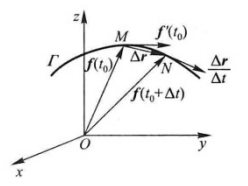
\includegraphics[width=4cm]{/media/wu/file/stuuudy/notes/images/miscellaneous/9.7.png}
\end{center}

当\(\Delta t>0\)时,向量\(\Delta \br=\bff(t_0+\Delta t)-\bff(t_0)\)的指向与\(t\)增大
是点\(M\)的移动走向一致,不论\(\Delta t>0\)或\(\Delta t<0\),向量\(\frac{\Delta \br}{\Delta
      t}\)的指向总与\(t\)的增长方向一致。于是导向量\(\bff'(t_0)\)是向量值函数的
   终端曲线在点\(M\)处的一个切向量,指向与\(t\)的增长方向一致


设空间曲线 \(\Gamma\) 的参数方程为
\begin{equation*}
\begin{cases}
x=\varphi(t)\\
y=\psi(t)\\
z=\omega(t)
\end{cases},t\in[\alpha,\beta]
\end{equation*}
假定三个函数在\([\alpha,\beta]\)可导且不同时为 0。向量
\(\bT=\bff'(t_0)=(\varphi'(t_0),\psi'(t_0),\omega'(t_0))\)是曲线 \(\Gamma\) 在点\(M\)
处的切向量,从而曲线 \(\Gamma\) 在点\(M\)处的 \textbf{切线方程} 为
\begin{equation*}
\frac{x-x_0}{\varphi'(t_0)}=
\frac{y-y_0}{\psi'(t_0)}=
\frac{z-z_0}{\omega'(t_0)}=
\end{equation*}
通过点\(M\)且与切线垂直的平面称为曲线 \(\Gamma\) 在点\(M\)处的 \textbf{法平面} , \textbf{法平面方程} 为
\begin{equation*}
\varphi'(t_0)(x-x_0)+\psi'(t_0)(y-y_0)+\omega'(t_0)(z-z_0)=0
\end{equation*}


给定曲面 \(\Sigma\) 方程
\begin{equation*}
F(x,y,z)=0
\end{equation*}
\(M(x_0,y_0,z_0)\)是曲面 \(\Sigma\) 一点,并设函数\(F(x,y,z)\)的偏导数在该点连续且不同
时为零,在曲面 \(\Sigma\) 上,通过点\(M\)任意因一条曲线 \(\Gamma\) ,假定曲线 \(\Gamma\) 的参数方程为
\begin{equation*}
x=\varphi(t),y=\psi(t),z=\omega(t)(\alpha\le t\le\beta)
\end{equation*}
\(t=t_0\)对应于点\(M\),则曲线切线方程为
\begin{equation*}
\frac{x-x_0}{\varphi'(t_0)}=
\frac{y-y_0}{\psi'(t_0)}=
\frac{z-z_0}{\omega'(t_0)}=
\end{equation*}
现在证明,在曲面 \(\Sigma\) 上通过点\(M\)且在点\(M\)处具有切线的任何曲线,它们在点
\(M\)处的切线都在同一平面。由恒等式
\begin{equation*}
F[\varphi(t),\psi(t),\omega(t)]\equiv0
\end{equation*}
因为\(F(x,y,z)\)在\(M\)有连续偏导数,且
\(\varphi'(t_0),\psi'(t_0),\omega'(t_0)\)存在,所以恒等式左边的复合函数在
\(t=t_0\)处有全导数,且这全导数等于零
\begin{equation*}
\left.\frac{d}{dt}F[\varphi(t),\psi(t),\omega(t)]\right\rvert_{t=t_0}=0
\end{equation*}
即有
\begin{equation*}
F_x(x_0,y_0,z_0)\varphi'(t_0)+
F_y(x_0,y_0,z_0)\psi'(t_0)+
F_z(x_0,y_0,z_0)\omega'(t_0)=0
\end{equation*}
引入向量
\begin{equation*}
\bn=(F_x(x_0,y_0,z_0),F_y(x_0,y_0,z_0),F_z(x_0,y_0,z_0))
\end{equation*}
切向量
\begin{equation*}
\bT=(\varphi'(t_0),\psi'(t_0),\omega'(t_0))
\end{equation*}
与\(\bn\)垂直。
因此切平面方程
\begin{equation*}
F_x(x_0,y_0,z_0)(x-x_0)+
F_y(x_0,y_0,z_0)(y-y_0)+
F_z(x_0,y_0,z_0)(z-z_0)=0
\end{equation*}
\subsection{方向导数与梯度}
\label{sec:org1bdf455}
\begin{theorem}[]
如果函数\(f(x,y)\)在点\(P_0(x_0,y_0)\)可微分,那么函数在该点沿任一方向\(l\)的
方向导数存在,且有
\begin{equation*}
\left.\frac{\partial f}{\partial l}\right\rvert_{(x_0,y_0)}=f_x(x_0,y_0)\cos\alpha+f_y(x_0,y_0)\cos\beta
\end{equation*}
其中\(\cos\alpha\)和\(\cos\beta\)是方向\(l\)的方向余弦
\end{theorem}

\begin{proof}
由假设\(f(x,y)\)在点\(x_0,y_0\)可微分,故有
\begin{align*}
&f(x_0+\Delta x,y_0+\Delta y)-f(x_0,y_0)\\
&=f_x(x_0,y_0)\Delta x+f_y(x_0,y_0)\Delta y+o(\sqrt{(\Delta x)^2+(\Delta y)^2})
\end{align*}
但点\((x_0+\Delta x,y_0+\Delta y)\)在以\((x_0,y_0)\)为始点的射线\(l\)上,应有
\(\Delta x=t\cos\alpha,\Delta y=t\cos\beta,\sqrt{(\Delta x)^2+(\Delta y)^2}=t\),所以
\begin{align*}
&\lim_{t\to0^+}\frac{f(x_0+t\cos\alpha,y_0+\cos\beta)-f(x_0,y_0)}{t}\\
&=f_x(x_0,y_0)\cos\alpha+f_y(x_0,y_0)\cos\beta
\end{align*}
\end{proof}

设函数\(f(x,y)\)在平面区域\(D\)内具有一阶连续偏导数,则对于\(P_0(x_0,y_0)\in
   D\),都可定出一个向量
\begin{equation*}
f_x(x_0,y_0)\bi+f_y(x_0,y_0)\bj
\end{equation*}
称为函数\(f(x,y)\)在点\(P_0(x_0,y_0)\)的 \textbf{梯度} ,记作\(\grad f(x_0,y_0)\)或
\(\nabla f(x_0,y_0)\),\(\nabla=\frac{\partial}{\partial x}\bi+\frac{\partial}{\partial y}\bj\)称为 \textbf{向量
微分算子}

设\(\be_l=(\cos\alpha,\cos\beta)\),则
\begin{align*}
\left.\frac{\partial f}{\partial l}\right\rvert_{(x_0,y_0)}&=
f_x(x_0,y_0)\cos\alpha+f_y(x_0,y_0)\cos\beta\\
&=\grad f(x_0,y_0)\cdot\be_l=\abs{\grad f(x_0,y_0)}\cos\theta
\end{align*}
其中\(\theta=\la\grad f(x_0,y_0),\be_l\ra\)
\subsection{多元函数的梯度及其求法}
\label{sec:orgfab37cc}
\begin{definition}[]
设函数\(z=f(x,y)\)的定义域为\(D\),\(P_0(x_0,y_0)\)为\(D\)的内点,若存在
\(P_0\)的某个邻域\(U(P_0)\subset D\)使得对于该邻域内异于\(P_0\)的任何点
\((x,y)\)都有
\begin{equation*}
f(x,y)<f(x_0,y_0)
\end{equation*}
则称函数\(f(x,y)\)在点\((x_0,y_0)\)有 \textbf{极大值} \(f(x_0,y_0)\),点\((x_0,y_0)\)
称为 \textbf{极大值点} 。极大值极小值统称为 \textbf{极值}
\end{definition}

\begin{theorem}[必要条件]
设函数\(z=f(x,y)\)在点\((x_0,y_0)\)有偏导数,且在点\((x_0,y_0)\)处有极值,则
有
\begin{equation*}
f_x(x_0,y_0)=0,f_y(x_0,y_0)=0
\end{equation*}
\end{theorem}

凡是能使\(f_x(x_0,y_0)=f_y(x_0,y_0)=0\)的点称为 \textbf{驻点}

\begin{definition}[充分条件]
设函数\(z=f(x,y)\)在点\((x_0,y_0)\)的某邻域内有连续且有一阶及二阶连续偏导数,
又\(f_x(x_0,y_0)=0,f_y(x_0,y_0)=0\),令
\begin{equation*}
f_{xx}(x_0,y_0)=A,f_{xy}(x_0,y_0)=B,f_{yy}(x_0,y_0)=C
\end{equation*}
则
\begin{enumerate}
\item \(AC-B^2>0\)时有极值,且当\(A<0\)时有极大值,\(A>0\)时有极小值
\item \(AC-B^2<0\)无极值
\item \(AC-B^2=0\)可能有极值,可能没极值
\end{enumerate}
\end{definition}

寻求函数
\begin{equation*}
z=f(x,y)
\end{equation*}
在条件
\begin{equation*}
\varphi(x,y)=0
\end{equation*}
下取得极值的必要条件

如果函数在\((x_0,y_0)\)取得所求的极值,那么首先有
\begin{equation*}
\varphi(x_0,y_0)=0
\end{equation*}
假定在\((x_0,y_0)\)的某一邻域内\(f(x,y)\)与\(\varphi(x,y)\)均有连续的一阶偏导数,而
\(\varphi_x(x_0,y_0)\neq0\),由隐函数存在定理可知,\(\varphi(x,y)=0\)确定一个连续且
具有连续导数的函数\(y=\psi(x)\),得
\begin{equation*}
z=f[x,\psi(x)]
\end{equation*}
又取得极值的必要条件可知
\begin{equation*}
\left.\frac{dz}{dx}\right\rvert_{x=x_0}=f_x(x_0,y_0)+f_y(x_0,y_0)
\left.\frac{dy}{dx}\right\rvert_{x=x_0}=0
\end{equation*}
而由隐函数求导可知
\begin{equation*}
\left.\frac{dy}{dx}\right\rvert_{x=x_0}=
-\frac{\varphi_x(x_0,y_0)}{\varphi_y(x_0,y_0)}
\end{equation*}

代入得
\begin{equation*}
f_x(x_0,y_0)-f_y(x_0,y_0)\frac{\varphi_x(x_0,y_0)}{\varphi_y(x_0,y_0)}=0
\end{equation*}
设 \(\frac{f_y(x_0,y_0)}{\varphi_y(x_0,y_0)}=-\lambda\),则上述条件变为
\begin{equation*}
\begin{cases}
f_x(x_0,y_0)+\lambda\varphi_x(x_0,y_0)=0\\
f_y(x_0,y_0)+\lambda\varphi_y(x_0,y_0)=0\\
\varphi(x_0,y_0)=0
\end{cases}
\end{equation*}


\textbf{拉格朗日乘数法} 。要找函数\(z=f(x,y)\)在附加条件\(\varphi(x,y)=0\)下的可能极值点,可
以先作拉格朗日函数
\begin{equation*}
L(x,y)=f(x,y)+\lambda\varphi(x,y)
\end{equation*}
其中 \(\lambda\) 为参数,求其对\(x,y\)的一阶偏导数,并使之为零,然后与方程联立
\begin{equation*}
\begin{cases}
f_x(x,y)+\lambda\varphi_x(x,y)=0\\
f_y(x,y)+\lambda\varphi_y(x,y)=0\\
\varphi(x,y)=0
\end{cases}
\end{equation*}
解出\(x,y,\lambda\)就是可能极值点

\(\lambda\) 称为 \textbf{拉格朗日乘子} ,\(L\)称为 \textbf{拉格朗日函数}
\section{重积分}
\label{sec:orgedb034b}
\subsection{二重积分的概念与性质}
\label{sec:org815fe51}
\begin{definition}[]
设\(f(x,y)\)是有界闭区域\(D\)上的有界函数,将闭区域\(D\)任意分成\(n\)个小闭区
域
\begin{equation*}
\Delta\sigma_1,\dots,\Delta\sigma_n
\end{equation*}
其中\(\Delta \sigma_i\)表示第\(i\)个小闭区域,也表示它的面积,在每个\(\Delta \sigma_i\)
上任取一点\((\xi_i,\eta_i)\)作乘积\(f(\xi_i,\eta_i)\Delta \sigma_i\),并作和
\(\sum_{i=1}^nf(\xi_i,\eta_i)\Delta\sigma_i\),如果当各小闭区域的直径中的最大
值\(\lambda\to0\)时,这和的极限总存在,且与闭区域\(D\)的分法及点
\((\xi_i,\eta_i)\)的取法无关,那么称此极限为函数\(f(x,y)\)在闭区域\(D\)上的
\textbf{二重积分} ,记作 \(\iint_Df(x,y)d\sigma\),即
\begin{equation*}
\iint_Df(x,y)d\sigma=\lim_{\lambda\to0}\sum_{i=1}^n
f(\xi_i,\eta_i)\Delta\sigma_i
\end{equation*}
其中\(f(x,y)\)叫做 \textbf{被积函数} ,\(f(x,y)d\sigma\)叫做 \textbf{被积表达式} ,\(d\sigma\)
叫做 \textbf{面积元素} ,\(x,y\)叫做 \textbf{积分变量} ,\(D\)叫做 \textbf{积分区域} ,
\(\sum_{i=1}^nf(\xi_i,\eta_i)\Delta\sigma_i\)叫做 \textbf{积分和}
\end{definition}

设矩形区域\(\Delta \sigma_i\)的变长为\(\Delta x_j,\Delta y_k\),则\(\Delta \sigma_i=\Delta
   x_j\cdot\Delta y_k\)。因此有时也把面积元素\(d\sigma\)记作\(dxdy\),而把二重积
分记作
\begin{equation*}
\iint_Df(x,y)dxdy
\end{equation*}
\(dxdy\)叫做直角座标系的面积元素

\begin{proposition}[]
设 \(\alpha\),\(\beta\) 为常数,则
\begin{equation*}
\iint_D[\alpha f(x,y)+\beta g(x,y)]d\sigma=\alpha\iint_Df(x,y)d\sigma+
\beta\iint_Dg(x,y)d\sigma
\end{equation*}
\end{proposition}

\begin{proposition}[可加性]
如果闭区域\(D\)被有限条曲线分成有限个部分闭区域,那么在\(D\)上的二重积分等于
在各部分闭区域上的二重积分的和
\end{proposition}

\begin{proposition}[]
如果在\(D\)上\(f(x,y)=1\), \(\sigma\) 为\(D\)的面积,那么
\begin{equation*}
\sigma=\iint_D1\cdot d\sigma=\iint_Dd\sigma
\end{equation*}
\end{proposition}

\begin{proposition}[]
如果在\(D\)上,\(f(x,y)\le g(x,y)\),那么有
\begin{equation*}
\iint_Df(x,y)d\sigma\le \iint_Dg(x,y)d\sigma
\end{equation*}
特殊地,由于
\begin{equation*}
-\abs{f(x,y)}\le f(x,y)\le\abs{f(x,y)}
\end{equation*}
又有
\begin{equation*}
\abs{\iint_Df(x,y)d\sigma}\le\iint\abs{f(x,y)}d\sigma
\end{equation*}
\end{proposition}

\begin{proposition}[]
设\(M,m\)分别是\(f(x,y)\)在闭区域\(D\)上的最大值和最小值, \(\sigma\) 是\(D\)的面积,
则有
\begin{equation*}
m\sigma\le\iint_Df(x,y)d\sigma\le M\sigma
\end{equation*}
\end{proposition}

\begin{proposition}[二重积分的中值定理]
设函数\(f(x,y)\)在闭区域\(D\)上连续, \(\sigma\) 是\(D\)的面积,则在\(D\)上至少存在一
点\((\xi,\eta)\)使得
\begin{equation*}
\iint_Df(x,y)d\sigma=f(\xi,\eta)\sigma
\end{equation*}
\end{proposition}
\subsection{二重积分的计算法}
\label{sec:org7b860f0}
\begin{center}
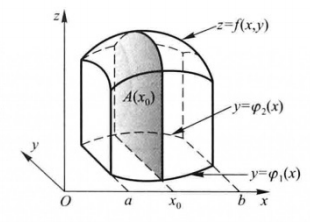
\includegraphics[width=4cm]{/media/wu/file/stuuudy/notes/images/miscellaneous/10.5.png}
\end{center}
现计算截面面积,
\begin{equation*}
A(x)=\int_{\varphi_1(x)}^{\varphi_2(x)}f(x,y)dy
\end{equation*}
则体积
\begin{equation*}
V=\int_a^bA(x)dx=\int_a^b\left[
\int_{\varphi_1(x)}^{\varphi_2(x)}f(x,y)dy
\right]dx=\iint_Df(x,y)d\sigma
\end{equation*}

\begin{center}
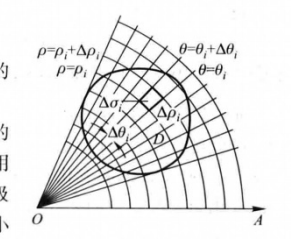
\includegraphics[width=4cm]{/media/wu/file/stuuudy/notes/images/miscellaneous/10.17.png}
\end{center}
把\(D\)分成\(n\)各小闭区域,则
\begin{align*}
\Delta \sigma_i&=\frac{1}{2}(\rho_i+\Delta\rho_i)^2\cdot\Delta\theta_i-\frac{1}{2}\rho_i^2\cdot\Delta
\theta_i=\frac{1}{2}(2\rho_i+\Delta\rho_i)\Delta\rho_i\cdot\Delta\theta_i\\
&=\frac{\rho_i+(\rho_i+\Delta\rho_i)}{2}\cdot\Delta\rho_i\cdot\Delta\theta_i=
\bbar{\rho}_i\cdot\Delta\rho_i\cdot\Delta\theta_i
\end{align*}
其中\(\bbar{\rho}_i\)表示相邻两圆弧的半径的平均值,在小闭区域内取圆周
\(\rho=\bbar{\rho}_i\)上的一点\(\bbar{\rho_i},\bbar{\theta_i}\),该点的直角坐标
设为\((\xi_i,\eta_i)\),则\(\xi_i=\bbar{\rho_i}\cos\bbar{\theta_i}\),
\(\eta_i=\bbar{\rho_i}\sin\bbar{\theta_i}\),于是
\begin{equation*}
\iint_Df(x,y)d\sigma=\iint_Df(\rho\cos\theta,\rho\sin\theta)\rho d\rho d\theta
\end{equation*}
其中\(\rho d\rho d\theta\)就是 \textbf{极坐标系中的面积元素}

\begin{examplle}[]
计算\(\iint_De^{-x^2-y^2}dxdy\),其中\(D\)是由圆心在原点、半径为\(a\)的圆周所
围成的闭区域


\begin{align*}
\iint_De^{-x^2-y^2}dxdy&=
\iint_De^{-\rho^2}\rho d\rho d\theta=\int_0^{2\pi}d\theta\int_0^ae^{-\rho^2}\rho d\rho\\
&=\pi(1-e^{-a^2})
\end{align*}

下面来计算\(\int_0^{+\infty}e^{-x^2}dx\)

\begin{center}
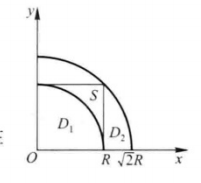
\includegraphics[width=4cm]{/media/wu/file/stuuudy/notes/images/miscellaneous/10.22.png}
\end{center}
设
\begin{align*}
&D_1=\{(x,y)\mid x^2+y^2\le R^2,x\ge0,y\ge0\}\\
&D_2=\{(x,y)\mid x^2+y^2\le 2R^2,x\ge0,y\ge0\}\\
&S=\{(x,y)\mid 0\le x\le R,0\le y\le R\}
\end{align*}
从而
\begin{equation*}
\iint_{D_1}e^{-x^2-y^2}dxdy<\iint_Se^{-x^2-y^2}dxdy<\iint_{D_2}e^{-x^2-y^2}dxdy
\end{equation*}
而
\begin{equation*}
\iint_Se^{-x^2-y^2}dxdy=\int_0^Re^{-x^2}dx\cdot\int_0^Re^{-y^2}dy=
(\int_0^Re^{-x^2}dx)^2
\end{equation*}
从而
\begin{equation*}
\frac{\pi}{4}(1-e^{-R^2})<(\int_0^Re^{-x^2}dx)^2<\frac{\pi}{4}(1-e^{2R^2})
\end{equation*}
当\(R\to+\finty\)时
\begin{equation*}
\int_0^{+\infty}e^{-x^2}dx=\frac{\sqrt{\pi}}{2}
\end{equation*}
\end{examplle}
\subsection{三重积分}
\label{sec:orgba3611f}
设\(M(x,y,z)\)为空间内一点,并设点\(M\)在\(xOy\)面上的投影\(P\)的极坐标为
\(\rho,\theta,z\),这样的三个数叫做点 \(M\)的 \textbf{柱面坐标} ,于是
\begin{equation*}
dv=\rho d\rho d\theta dz
\end{equation*}
\textbf{柱面坐标系中的体积元素} ,因此
\begin{equation*}
\iiint_\Omega f(x,y,z)dxdydz=\iiint_{\Omega}f(\rho\cos\theta,\rho\sin\theta,z)\rho
d \rho d\theta
\end{equation*}


\begin{center}
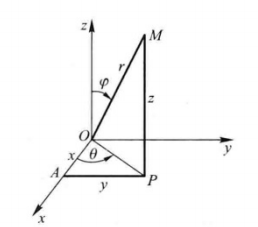
\includegraphics[width=4cm]{/media/wu/file/stuuudy/notes/images/miscellaneous/10.35.png}
\end{center}
则
\begin{equation*}
\begin{cases}
x=OP\cos\theta=r\sin\varphi\cos\theta\\
y=OP\sin\theta=r\sin\varphi\sin\theta\\
z=r\cos\varphi
\end{cases}
\end{equation*}

\begin{equation*}
\iiint_\Omega f(x,y,z)dxdydz=
\iiint_\Omega F(r,\rho,\theta)r^2\sin\varphi drd\varphi d\theta
\end{equation*}
其中\(F(r,\varphi,\theta)=f(r\sin\varphi\cos\theta,r\sin\varphi\sin\theta,r\cos\varphi)\)
\subsection{重积分的应用}
\label{sec:orgbbc438d}
设曲面\(S\)由方程
\begin{equation*}
z=f(x,y)
\end{equation*}
给出,\(D\)为曲面\(S\)在\(xOy\)面上的投影区域,函数\(f(x,y)\)在\(D\)上具有连
续偏导数\(f_x(x,y),f_y(x,y)\),要计算曲面\(S\)的面积\(A\)

\begin{center}
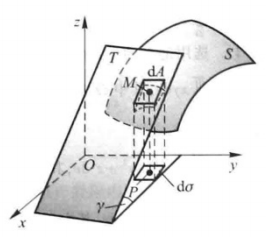
\includegraphics[width=4cm]{/media/wu/file/stuuudy/notes/images/miscellaneous/10.38.png}
\end{center}

在闭区域\(D\)上取一直径很小的闭区域 \(d\sigma\),在\(d\sigma\)上取一点
\(P(x,y)\),曲面\(S\)上对应地有一点\(M(x,y,f(x,y))\),\(P\)处曲面\(S\)的切平
面设为\(T\),以小闭区域\(d\sigma\)的边界为准线作母线平行于\(z\)轴的柱面,这柱
面在曲面\(S\)上截下一小片曲面,在切平面\(T\)上截下一小片平面,由于\(d\sigma\)
直径很小,切平面\(T\)上的那一小片平面的面积\(dA\)可以近似代替相应的曲面面积,
设点\(M\)处曲面\(S\)上的法线(指向朝上)与\(z\)轴所成的角为 \(\gamma\) ,则
\begin{equation*}
dA=\frac{d\sigma}{\cos\gamma}
\end{equation*}
因为
\begin{equation*}
\cos\gamma=\frac{1}{\sqrt{1+f_x^2(x,y)+f_y^2(x,y)}}
\end{equation*}
所以
\begin{equation*}
dA=\sqrt{1+f_x^2(x,y)+f_y^2(x,y)}d\sigma
\end{equation*}
这就是 \textbf{曲面\(S\)的面积元素} ,于是
\begin{equation*}
A=\iint_D\sqrt{1+f_x^2(x,y)+f_y^2(x,y)}d\sigma
\end{equation*}
或
\begin{equation*}
A=\iint_D\sqrt{1+(\frac{\partial z}{\partial x})^2+(\frac{\partial z}{\partial y})^2}dxdy
\end{equation*}
设曲面的方程\(x=g(y,z),y=h(z,x)\)可分别把曲面投影到\(yOz,zOx\)平面上,则
\begin{equation*}
A=\iint_{D_{yz}}\sqrt{1+(\frac{\partial x}{\partial y})^2+(\frac{\partial x}{\partial z})^2}dydz
\end{equation*}
或
\begin{equation*}
A=\iint_{D_{zx}}\sqrt{1+(\frac{\partial y}{\partial z})^2+(\frac{\partial y}{\partial x})^2}dzdx
\end{equation*}

\begin{examplle}[]
求半径为\(a\)的球的表面积

取上半球面方程为\(z=\sqrt{a^2-x^2-y^2}\),它在\(xOy\)面上的投影区域
\(D=\{(x,y)\mid x^2+y^2\le a^2\}\)
\begin{equation*}
\sqrt{1+(\frac{\partial z}{\partial x})^2+(\frac{\partial z}{\partial y})^2}=\frac{1}{\sqrt{a^2-x^2-y^2}}
\end{equation*}

因为这个函数在闭区域\(D\)上无界,所以先取\(D_1=\{(x,y)\mid x^2+y^2\le b^2\}\)
,之后令\(b\to a\)
\begin{align*}
A_1=\iint_{D_1}\frac{a}{\sqrt{a^2-\rho^2}}\rho d\rho d\theta=
a\int_0^{2\pi}d\theta\int_0^b\frac{\rho d\rho}{\sqrt{a^2-\rho^2}}\\
&=2\pi a(a-\sqrt{a^2-b^2})
\end{align*}
于是
\begin{equation*}
\lim_{b\to a}A_1=2\pi a^2
\end{equation*}
\end{examplle}
\section{曲线积分与曲面积分}
\label{sec:orgedbab1f}
\subsection{对弧长的曲线积分}
\label{sec:org214024e}
\begin{definition}[]
设\(L\)为\(xOy\)面内的一条光滑曲线弧,函数\(f(x,y)\)在\(L\)上有界,在\(L\)上任
意插入一点列\(M_1,\dots,M_{n-1}\)把\(L\)分成\(n\)个小段,设第\(i\)个小段的长度
为\(\Delta s_i\),又\((\xi_i,\eta_i)\)为第\(i\)个小段上任意取定的一点,作乘积
\(f(\xi_i,\eta_i)\Delta s_i\),并作和\(\sum_{i=1}^nf(\xi_i,\eta_i)\Delta s_i\),如果当各
小段弧段的长度的最大值\(\lambda\to0\)时,这和的极限总存在,且与曲线弧\(L\)的分
法及点\((\xi_i,\eta_i)\)的取法无关,那么称此极限为函数\(f(x,y)\)在曲线弧\(L\)
上 \textbf{对弧长的曲线积分} 或 \textbf{第一类曲线积分} ,记作\(\int_Lf(x,y)ds\),即
\begin{equation*}
\int_Lf(x,y)=ds=\lim_{\lambda\to0}\sum_{i=1}^nf(\xi_i,\eta_i)\Delta s_i
\end{equation*}
其中\(f(x,y)\)叫做 \textbf{被积函数} ,\(L\)叫做 \textbf{积分弧段}
\end{definition}

\begin{proposition}[]
设 \(\alpha\),\(\beta\) 为常数,则
\begin{equation*}
\int_L[\alpha f(x,y)+\beta g(x,y)]ds=\alpha\int_Lf(x,y)ds+\beta\int_Lg(x,y)ds
\end{equation*}
\end{proposition}

\begin{proposition}[]
若积分弧段\(L\)可分成两端光滑曲线弧\(L_1,L_2\),则
\begin{equation*}
\int_Lf(x,y)ds=\int_{L_1}f(x,y)ds+\int_{L_2}f(x,y)ds
\end{equation*}
\end{proposition}

\begin{proposition}[]
设在\(L\)上\(f(x,y)\le g(x,y)\),则
\begin{equation*}
\int_Lf(x,y)ds\le\int_Lg(x,y)ds
\end{equation*}
特别地,有
\begin{equation*}
\abs{\int_Lf(x,y)ds}\le\int_L\abs{f(x,y)}ds
\end{equation*}
\end{proposition}

\begin{theorem}[]
设\(f(x,y)\)在曲线弧\(L\)上有定义且连续,\(L\)的参数方程为
\begin{equation*}
\begin{cases}
x=\varphi(t)\\
y=\psi(t)
\end{cases}
(\alpha\le t\le\beta)
\end{equation*}
若\(\varphi(t),\psi(t)\)在\([\alpha,\beta]\)上具有一阶连续导数,且
\(\varphi'^2(t)+\psi'^2(t)\neq0\),则曲线积分\(\int_Lf(x,y)ds\)存在,且
\begin{equation*}
\int_Lf(x,y)ds=\int_\alpha^\beta f[\varphi(t),\psi(t)]\sqrt{\varphi'^2(t)
+\psi'^2(t)}dt(\alpha<\beta)
\end{equation*}
\end{theorem}

如果曲线弧\(L\)由方程
\begin{equation*}
y=\psi(x)(x_0\le x\le X)
\end{equation*}
可以看成
\begin{equation*}
x=t,y=\psi(t)
\end{equation*}
\subsection{对坐标的曲线积分}
\label{sec:org4885760}
\begin{definition}[]
设\(L\)为\(xOy\)面从点\(A\)到点\(B\)的一条有向光滑曲线弧,函数\(P(x,y)\)与
\(Q(x,y)\)在\(L\)上有界,在\(L\)上沿\(L\)的方向任意插入一点列
\(M_1(x_1,y_1),d\ots,M_{n-1}(x_{n-1},y_{n-1})\),把\(L\)分成\(n\)个有向小弧段
\(\arc{M_{i-1}M_i}\).设 \(\Delta x_i=x_i-x_{i-1},\Delta y_i=y_i-y_{i-1}\),点
\((\xi_i,\eta_i)\)为\(\arc{M_{i-1}M_i}\)任意取定的点,作乘积
\(P(\xi_i,\eta_i)\Delta x_i\),并作和\(\sum_{i=1}^nP(\xi_i,\eta_i)\Delta x_i\),如果当
各小弧段长度的最大值\(\lambda\to0\)时这和的极限总存在,且与曲线弧\(L\)的分法
及点\((\xi_i,\eta_i)\)的取法无关,那么称此极限为函数\(P(x,y)\)在有向曲线弧
\(L\)上 \textbf{对坐标\(x\)的曲线积分} ,记作\(\int_LP(x,y)dx\)。
\begin{align*}
&\int_LP(x,y)dx=\lim_{\lambda\to0}\sum_{i=1}^nP(\xi_i,\eta_i)\Delta x_i\\
&\int_LQ(x,y)dy=\lim_{\lambda\to0}\sum_{i=1}^nQ(\xi_i,\eta_i)\Delta y_i\\
\end{align*}
其中\(P(x,y),Q(x,y)\)叫做 \textbf{被积函数} ,\(L\)叫做 \textbf{积分弧段} 

\textbf{第二类曲线积分}
\end{definition}

应用上经常出现
\begin{equation*}
\int_LP(x,y)dx+\int_LQ(x,y)dy
\end{equation*}
合并起来可写成向量形式
\begin{equation*}
\int_L\bF(x,y)\cdot d\br
\end{equation*}
其中\(\bF(x,y)=P(x,y)\bi+Q(x,y)\bj\),\(d\br=dx\bi+dy\bj\)

\begin{proposition}[]
设 \(\alpha\),\(\beta\) 为常数,则
\begin{equation*}
\int_L[\alpha\bF_1(x,y)+\beta\bF_2(x,y)]\cdot d\br=
\alpha\int_L\bF_1(x,y)\cdot\br+\beta\int_L\bF_2(x,y)\cdot d\br
\end{equation*}
\end{proposition}

\begin{proposition}[]
若有向曲线弧\(L\)可分成两段光滑的有向曲线弧\(L_1,L_2\),则
\begin{equation*}
\int_L\bF(x,y)\cdot d\br=\int_{L_1}\bF(x,y)\cdot d\br+
\int_{L_2}\bF(x,y)\cdot d\br
\end{equation*}
\end{proposition}

\begin{proposition}[]
设\(L\)是有向光滑曲线弧,\(L^-\)是\(L\)的反向曲线弧,则
\begin{equation*}
\int_{L^-}\bF(x,y)\cdot d\br=-\int_L\bF(x,y)\cdot d\br
\end{equation*}
\end{proposition}

\begin{theorem}[]
设\(P(x,y),Q(x,y)\)在有向曲线弧\(L\)上有定义且连续,\(L\)的参数方程
\begin{equation*}
\begin{cases}
x=\varphi(t)\\
y=\psi(t)
\end{cases}
\end{equation*}
当参数\(t\)单调地由 \(\alpha\) 变到 \(\beta\) 时,点\(M(x,y)\) 从\(L\)的起点\(A\)沿\(L\)运动到
终点\(B\),若\(\varphi(t),\psi(t)\)在以 \(\alpha\) 及 \(\beta\) 为端点的闭区间上具有一阶连续导数,且
\(\varphi'^2(t)+\psi'^2(t)\neq0\),则曲线积分\(\int_LP(x,y)dx+Q(x,y)dy\)存在,
且
\begin{align*}
&\int_LP(x,y)dx+Q(x,y)dy\\
&=\int_\alpha^\beta\{P[\varphi(t),\psi(t)]\varphi'(t)+Q[\varphi(t),\psi(t)]\psi'(t)\}dt
\end{align*}
\end{theorem}
\subsection{格林公式及其应用}
\label{sec:orga6403b6}
设\(D\)为平面区域,若\(D\)内任一闭曲线所围成的部分都属于\(D\),则称\(D\)为平
面 \textbf{单连通区域} ,否则称为 \textbf{复连通区域}

对平面区域\(D\)的边界曲线\(L\),我们规定\(L\)的正向如下:当观察者沿\(L\)的这
个方向行走时,\(D\)内在他近处的那一部分总在他的左边
\begin{theorem}[格林公式]
设闭区域\(D\)由分段光滑的曲线\(L\)围成,若函数\(P(x,y),Q(x,y)\)在\(D\)上具有
一阶连续偏导数,则有
\begin{equation*}
\iint_D(\frac{\partial Q}{\partial x}-\frac{\partial P}{\partial y})dxdy=\oint_LPdx+Qdy
\end{equation*}
其中\(L\)是\(D\)的取正向的边界曲线
\end{theorem}

取\(P=-y,Q=x\),即得
\begin{equation*}
2\iint_Ddxdy=\oint_Lxdy-ydx
\end{equation*}
因此
\begin{equation*}
A=\frac{1}{2}\oint_Lxdy-ydx
\end{equation*}


设\(G\)是一个区域,\(P(x,y)\)以及\(Q(x,y)\)在区域\(G\)内具有一阶连续偏导数,
如果对于\(G\)内任意指定的两个点\(A,B\)以及\(G\)内从\(A\)到点\(B\)的任意两条曲
线\(L_1,L_2\),等式
\begin{equation*}
\int_{L_1}Pdx+Qdy=\int_{L_2}Pdx+Qdy
\end{equation*}
恒成立,就说 \textbf{曲线积分} \(\int_LPdx+Qdy\) \textbf{在\(G\)内与路径无关}

\begin{theorem}[]
设区域\(G\)是一个单连通域,若函数\(P(x,y)\)与\(Q(x,y)\)在\(G\)内具有一阶连续
偏导数,则曲线积分\(\int_LPdx+Qdy\)在\(G\)内与路径无关的充分必要条件是
\begin{equation*}
\frac{\partial P}{\partial y}=\frac{\partial Q}{\partial x}
\end{equation*}
在\(G\)内恒成立
\end{theorem}

\begin{theorem}[]
设区域\(G\)是一个单连通域,若函数\(P(x,y),Q(x,y)\)在\(G\)内具有一阶连续偏导数,
则\(P(x,y)dx+Q(x,y)dy\)在\(G\)内为某一函数\(u(x,y)\)的全微分的充分必要条件是
\begin{equation*}
\frac{\partial P}{\partial y}=\frac{\partial Q}{\partial x}
\end{equation*}
在\(G\)内恒成立
\end{theorem}
\subsection{对面积的曲面积分}
\label{sec:orgb8a4bd7}
\begin{definition}[]
设曲面 \(\Sigma\) 是光滑的,函数\(f(x,y,z)\)在 \(\Sigma\) 上有界,把 \(\Sigma\) 任意分成\(n\)小块
\(\Delta S_i\),设\((\xi_i,\eta_i,\zeta_i)\Delta S_i\),并作和
\(\sum_{i=1}^nf(\xi_i,\eta_i,\zeta_i)\Delta S_i\),如果当各小块曲面的直径的最大值
\(\lambda\to0\)时,这和的极限总存在,且与曲面 \(\Sigma\) 的分法及点
\((\xi_i,\eta_i,\zeta_i)\)的取法无关,那么称此极限为函数\(f(x,y,z)\)在曲面 \(\Sigma\)
上 \textbf{对曲面的曲面积分} 或 \textbf{第一类曲面积分} ,记作\(\iint_\Sigma f(x,y,z)dS\),即
\begin{equation*}
\iint_\Sigma f(x,y,z)dS=\lim_{\lambda\to0}\sum_{i=1}^nf(\xi_i,\eta_i,\xi_i)\Delta S_i
\end{equation*}
其中\(f(x,y,z)\)叫做 \textbf{被积函数} , \(\Sigma\)  叫做 \textbf{积分曲面}
\end{definition}

\begin{align*}
&   \iint_\Sigma f(x,y,z)dS=\\
&=\iint_{Dxy}f[x,y,z(x,y)]\sqrt{1+z_x^2(x,y)+z_y^2(x,y)}dxdy
\end{align*}
\subsection{对坐标的曲面积分}
\label{sec:org47159ed}
\textbf{第二类曲面积分}
\begin{align*}
&\iint_\Sigma R(x,y,z)dxdy=\lim_{\lambda\to0}\sum_{i=1}^nR(\xi_i,\eta_i,\zeta_i)(\Delta S_i)_{xy}\\
&\iint_\Sigma R(x,y,z)dydz=\lim_{\lambda\to0}\sum_{i=1}^nR(\xi_i,\eta_i,\zeta_i)(\Delta S_i)_{yz}\\
&\iint_\Sigma R(x,y,z)dzdx=\lim_{\lambda\to0}\sum_{i=1}^nR(\xi_i,\eta_i,\zeta_i)(\Delta S_i)_{zx}
\end{align*}
\subsection{高斯公式}
\label{sec:org23df528}
\begin{theorem}[高斯公式]
设空间闭区域 \(\Omega\) 是由分片光滑的闭曲面 \(\Sigma\) 所围成,若函数
\(P(x,y,z),Q(x,y,z),R(x,y,z)\)在 \(\Omega\) 上具有一阶连续偏导数,则有
\begin{equation*}
\iiint_\Omega(\frac{\partial P}{\partial x}+\frac{\partial Q}{\partial y}+\frac{\partial R}{\partial z})dv=
\oiint_\Sigma Pdydz+Qdzdx+Rdxdy
\end{equation*}
或
\begin{equation*}
\iiint_\Omega(\frac{\partial P}{\partial x}+\frac{\partial Q}{\partial y}+\frac{\partial R}{\partial z})dv=
\oiint_\Sigma(P\cos\alpha+Q\cos\beta+R\cos\gamma)dS
\end{equation*}
这里 \(\Sigma\) 是 \(\Omega\) 的整个边界曲面的外侧,\(\cos\alpha,\cos\beta,\cos\gamma\)是 \(\Sigma\) 在
点\((x,y,z)\)处的法向量的方向余弦
\end{theorem}
\subsection{斯托克斯公式}
\label{sec:org931d569}
\begin{theorem}[斯托克斯公式]
设 \(\Gamma\) 为分段光滑的空间有向闭曲线, \(\Sigma\) 是以 \(\Gamma\) 为边界的分片光滑的有向曲面, \(\Gamma\) 的
正向与 \(\Sigma\) 的侧符合右手规则,若函数\(P(x,y,z),Q(x,y,z),R(x,y,z)\)在曲面 \(\Sigma\) (连
同边界 \(\Gamma\) )上具有一阶连续偏导数,则有
\begin{align*}
&\iint_\Sigma(\frac{\partial R}{\partial y}-\frac{\partial Q}{\partial z})dydz+
(\frac{\partial P}{\partial z}-\frac{\partial R}{\partial x})dzdx+
(\frac{\partial Q}{\partial x}-\frac{\partial P}{\partial y})dxdy\\
&\quad=\oint_\Gamma Pdx+Qdy+Rdz
\end{align*}
\end{theorem}
\section{无穷级数}
\label{sec:org57e88f5}
\subsection{常数项奇数的概念和性质}
\label{sec:org7278640}
\begin{definition}[]
如果级数\(\sum_{i=1}^\infty u_i\)的部分和数列\(\{s_n\}\)有极限\(s\),那么称无
穷级数\(\sum_{i=1}^\infty u_i\) \textbf{收敛} ,这时极限\(s\)叫做这级数的 \textbf{和} ,反之称
\textbf{发散}
\end{definition}

\begin{proposition}[]
如果级数 \(\sum_{n=1}^\infty u_n\)收敛于和\(s\),那么级数\(\sum_{n=1}^\infty
   ku_n\)也收敛,且其和为\(ks\)
\end{proposition}

\begin{proposition}[]
如果级数\(\sum_{n=1}^\infty u_n,\sum_{n=1}^\infty v_n\)分别收敛于\(s,\sigma\),
那么级数\(\sum_{n=1}^\infty(u_n\pm v_n)\)也收敛,且其和为\(s\pm\sigma\)
\end{proposition}

\begin{proposition}[]
在级数中去掉、加上或改变有限项,不改变级数的收敛性
\end{proposition}

\begin{proposition}[]
如果级数\(\sum_{n=1}^\infty u_n\)收敛,那么对这级数的项任意加括号所成的级数
\begin{equation*}
(u_1+\dots+u_{n_1})+(u_{n_1+1}+\dots+u_{n_2})+\dots+(
u_{n_{k-1}+1}+\dots+u_{n_k})+\dots
\end{equation*}
仍收敛,且其和不变
\end{proposition}

\begin{proof}
各项和是个子数列
\end{proof}

\begin{proposition}[级数收敛的必要条件]
如果级数\(\sum_{n=1}^\infty u_n\)收敛,那么它的一般项\(u_n\)趋于零,即
\begin{equation*}
\lim_{n\to+\infty}u_n=0
\end{equation*}
\end{proposition}

\begin{proof}
设级数\(\sum_{n=1}^\infty\)的部分和为\(s_n\),且\(s_n\to s(n\to\infty)\)
\begin{equation*}
lim_{n\to\infty}u_n=\lim_{n\to\infty}(s_n-s_{n-1})=\lim_{n\to\infty}s_n-
\lim_{n\to\infty}s_{n-1}=s-s=0
\end{equation*}
\end{proof}
\subsection{常数项级数的审敛法}
\label{sec:orgb4c808f}
\begin{theorem}[]
正项级数\(\sum_{n=1}^\infty u_n\)收敛的充分必要条件是:它的部分和数列
\(\{s_n\}\)有界
\end{theorem}

\begin{theorem}[比较审敛法]
设\(\sum_{n=1}^\infty u_n,\sum_{n=1}^\infty v_n\)都是正项级数,且\(u_n\le
   v_n\),若级数\(\sum_{n=1}^\infty v_n\)收敛,则级数\(\sum_{n=1}^\infty u_n\)收
敛,反之,若级数\(\sum_{n=1}^\infty u_n\)发散,则级数\(\sum_{n=1}^\infty
   v_n\)发散
\end{theorem}

\begin{corollary}[]
设\(\sum_{n=1}^\infty u_n,\sum_{n=1}^\infty v_n\)都是正项级数,如果级数
\(\sum_{n=1}^\infty v_n\)收敛,且存在正整数\(N\),使得当\(n\ge N\)时有
\(u_n\le k v_n(k>0)\)成立,那么级数\(\sum_{n=1}^\infty u_n\)收敛
\end{corollary}

\begin{examplle}[]
讨论\(p\)级数
\begin{equation*}
1+\frac{1}{2^p}+\frac{1}{3^p}+\dots+\frac{1}{n^p}+\dots
\end{equation*}
的收敛性,其中常数\(p>0\)

由比较审敛法,当\(p\le1\)时发散

设\(p>1\),因为当\(k-1\le x\le k\),有\(\frac{1}{k^p}\le\frac{1}{x^p}\),所以
\begin{equation*}
\frac{1}{k^p}=\int_{k-1}^k\frac{1}{k^p}dx\le\int_{k-1}^k\frac{1}{x^p}dx
\end{equation*}
从而级数的部分和
\begin{align*}
s_n&=1+\sum_{k=2}^n\frac{1}{k^p}\le1+\sum_{k=2}^n\int_{k-1}^k\frac{1}{x^p}dx=
1+\int_1^n\frac{1}{x^p}dx\\
&=1+\frac{1}{p-1}(1-\frac{1}{n^{p-1}})<1+\frac{1}{p-1}
\end{align*}
\end{examplle}

\begin{theorem}[比较审敛法的极限形式]
设\(\sum_{n=1}^\infty u_n,\sum_{n=1}^\infty v_n\)都是正项级数
\begin{enumerate}
\item 如果\(\lim_{n\to\infty}\frac{u_n}{v_n}=l(0\le l<+\infty)\),且级数
\(\sum_{n=1}^\infty v_n\)收敛,那么级数\(\sum_{n=1}^\infty u_n\)收敛
\item 如果\(\lim_{n\to\infty}\frac{u_n}{v_n}=l>0\)或
\(\lim_{n\to\infty}\frac{u_n}{v_n}=+\infty\)
,且级数
\(\sum_{n=1}^\infty v_n\)发散,那么级数\(\sum_{n=1}^\infty u_n\)发散
\end{enumerate}
\end{theorem}

\begin{theorem}[比值审敛法]
设\(\sum_{n=1}^\infty u_n\)为正项级数,如果
\begin{equation*}
\lim_{n\to\infty}\frac{u_{n+1}}{u_n}=\rho
\end{equation*}
那么当\(\rho<1\)时级数收敛,\(\rho>1\)(或
\(\lim_{n\to\infty}\frac{u_{n+1}}{u_n}=\infty\))时级数发散,\(\rho=1\)时级数
可能收敛可能发散
\end{theorem}

\begin{theorem}[极限审敛法]
设\(\sum_{n=1}^\infty u_n\)为正项级数
\begin{enumerate}
\item 如果\(\lim_{n\to\infty}nu_n=l>0\)(或\(\lim_{n\to\infty}nu_n=+\infty\)),
那么级数\(\sum_{n=1}^\infty u_n\)发散
\item 如果\(p>1\)而\(\lim_{n\to\infty}n^pu_n=l(0\le l\le+\infty)\),那么级数
\(\sum_{n=1}^\infty u_n\)收敛
\end{enumerate}
\end{theorem}

\begin{theorem}[莱布尼茨定理]
如果交错级数\(\sum_{n=1}^\infty(-1)^{n-1}u_n\)满足
\begin{enumerate}
\item \(u_n\ge u_{n+1}\)
\item \(\lim_{n\to\infty}u_n=0\)
\end{enumerate}


那么级数收敛,且其和\(s\le u_1\),其余项\(r_n\)的绝对值\(\abs{r_n}\le u_{n+1}\)
\end{theorem}


如果级数\(\sum_{n=1}^\infty u_n\)各项的绝对值所构成的正项级数
\(\sum_{n=1}^\infty\abs{u_n}\)收敛,那么称级数\(\sum_{n=1}^\infty u_n\) \textbf{绝对
收敛} ;如果级数\(\sum_{n=1}^\infty u_n\)收敛,而级数
\(\sum_{n=1}^\infty\abs{u_n}\)发散,那么称级数\(\sum_{n=1}^\infty u_n\)
\textbf{条件收敛}

\begin{theorem}[]
如果级数绝对收敛,那么级数必定收敛
\end{theorem}

\begin{examplle}[]
\(\sum_{n=1}^\infty\frac{\sin n\alpha}{n^2}\)

因为\(\abs{\frac{\sin n\alpha}{n^2}}\le \frac{1}{n^2}\)
\end{examplle}
\subsection{幂级数}
\label{sec:org30f39c5}
如果给定一个定义在区间\(I\)上的函数列
\begin{equation*}
u_1(x),u_2(x),\dots,u_n(x),\dots
\end{equation*}
那么由这函数列构成的表达式
\begin{equation*}
u_1(x)+u_2(x)+\dots+u_n(x)+\dots
\end{equation*}
称为定义在区间\(I\)上的 ( \textbf{函数项} ) \textbf{无穷级数} ,简称为 ( \textbf{函数项} ) \textbf{级数}

如果在\(x_0\in I\)上收敛,\(x_0\)称为 \textbf{收敛点} ,否则 \textbf{发散点} 。收敛点的集合 \textbf{收
敛域} ,发散点的集合 \textbf{发散域}

\textbf{幂级数} 的形式
\begin{equation*}
\sum_{n=0}^na_nx^n=a_0+a_1x+\dots+a_nx^n+\dots
\end{equation*}

\begin{theorem}[阿贝尔定理]
如果级数\(\sum_{n=0}^\infty a_nx^n\)当 \(x=x_0(x_0\neq0)\)时收敛,那么适合不
等式\(\abs{x}<\abs{x_0}\)的一切\(x\)使这幂级数绝对收敛。反之,如果级数在
\(x_0\)发散,那么适合不等式\(\abs{x}>\abs{x_0}\)的一切\(x\)使这幂级数发散
\end{theorem}

\begin{corollary}[]
如果幂级数\(\sum_{n=0}^\infty a_nx^n\)不是仅在\(x=0\)一点收敛,也不是在整个数
轴上都收敛,那么必有一个确定的\(R\)存在使得
\begin{enumerate}
\item 当\(\abs{x}<R\)时,幂级数绝对收敛
\item 当\(\abs{x}>R\),幂级数发散
\item 当\(x=\pm R\),可能收敛,可能发散
\end{enumerate}
\end{corollary}

\(R\)叫做 \textbf{收敛半径} ,开区间\((-R,R)\)叫做 \textbf{收敛半径}

\begin{theorem}[]
如果
\begin{equation*}
\lim_{n\to\infty}\abs{\frac{a_{n+1}}{a_n}}=\rho
\end{equation*}
其中\(a_n,a_{n+1}\)是幂级数\(\sum_{n=0}^\infty a_nx^n\)的相邻两项的系数,那么
这幂级数的收敛半径
\begin{equation*}
R=
\begin{cases}
\frac{1}{\rho}&\rho\neq0\\
+\infty&\rho=0\\
0&\rho=+\infty
\end{cases}
\end{equation*}
\end{theorem}

\begin{proof}
考虑级数
\begin{equation*}
\abs{a_0}+\abs{a_1x}+\abs{a_2x^2}+\dots+\abs{a_nx^n}+\dots
\end{equation*}
这级数相邻两项之比为
\begin{equation*}
\frac{\abs{a_{n+1}x^{n+1}}}{\abs{a_nx^n}}=\abs{\frac{a_{n+1}}{a_n}}\abs{x}
\end{equation*}

\begin{enumerate}
\item 如果\(\lim_{n\to\infty}\abs{\frac{a_{n+1}}{a_n}}=\rho(\rho\neq0)\)存在,根
据比值审敛法,当\(\rho\abs{x}<1\)时即\(\abs{x}<\frac{1}{\rho}\)时,级数绝对收
敛
\end{enumerate}
\end{proof}


\section{Appendix}
\label{sec:orgc5f83ff}
\begin{appendices}
\subsection{Trigonometry}
\label{sec:orga68c4a3}
\begin{equation*}
\sec\alpha=\frac{1}{\cos\alpha},\quad\csc\alpha=\frac{1}{\sin\alpha}
\end{equation*}

Suppose we have two units \(\vec{u}=(\cos x,\sin x),\vec{v}=(\cos y,\sin
   y)\), then
\begin{equation*}
\vec{u}\cdot\vec{v}=\cos x\cos y+\sin x\sin y=\cos(x-y)
\end{equation*}
Hence by substitute \(-y\) for \(y\) or \(\frac{\pi}{2}-x\) for \(x\), we have
\begin{gather*}
\cos(x+y)=\cos x\cos y-\sin x\sin y\\
\sin(x+y)=\sin x\cos y+\cos x\sin y\\
\sin(x-y)=\sin x\cos y-\cos x\sin y
\end{gather*}

let \(x=y\), we have
\begin{gather*}
\sin 2x=2\sin x\cos x\\
\cos 2x=\cos^2x-\sin^2x=1-2\sin^2 x=2\cos^2-1\\
\tan 2x=\frac{2\tan x}{1-\tan^2x}
\end{gather*}
Hence we have
\begin{gather*}
\sin^2\frac{x}{2}=\frac{1-\cos x}{2}\\
\cos^2\frac{x}{2}=\frac{1+\cos x}{2}\\
\tan^2\frac{x}{2}=\frac{1-\cos x}{1+\cos x}
\end{gather*}

\begin{equation*}
\tan\frac{x}{2}=\frac{\sin\frac{x}{2}}{\cos\frac{x}{2}}=
\frac{2\sin^2\frac{x}{2}}{2\sin\frac{x}{2}\cos\frac{x}{2}}=
\frac{1-\cos x}{\sin x}=\csc x-\cot x
\end{equation*}

\end{appendices}
\section{Index}
\label{sec:org92ef479}
\renewcommand{\indexname}{}
\printindex
\end{document}
